% ------------------------------------------------------------------------------
% Este fichero es parte de la plantilla LaTeX para la realización de Proyectos
% Final de Grado, protegido bajo los términos de la licencia GFDL.
% Para más información, la licencia completa viene incluida en el
% fichero fdl-1.3.tex

% Copyright (C) 2012 SPI-FM. Universidad de Cádiz
% ------------------------------------------------------------------------------

En esta sección se presenta el catálogo de requisitos del sistema de información. Para ello se detallarán los actores del sistema, los requisitos funcionales, los requisitos de información, los requisitos no funcionales, las reglas de negocio y las diferentes alternativas tecnológicas.
\section{Catálogo de actores}
Un Rol es una clasificación mediante la cual se definen distintos privilegios de operación para los usuarios del sistema. Los Roles se encuentran predefinidos en el sistema y se detallan a continuación:
\begin{itemize}
\item \textbf{Rol Empleado:} Son los usuarios normales de la aplicación, ellos pueden hacer uso de todo el sistema exceptuando las funciones propias del administrador y de los médicos.
\end{itemize}
\begin{itemize}
\item \textbf{Rol Médico:} Son usuarios de la aplicación con el rol empleado pero sólo ellos pueden crear informes de los clientes.
\end{itemize}
\begin{itemize}
\item \textbf{Rol Administrador:} Es el usuario del sistema con más privilegios. Puede realizar las funciones de un empleado pero con este rol pueden hacer algunas tareas propias de un administrador. No puede realizar informes.
\end{itemize}

\section{Requisitos funcionales}
A continuación se detallan, a partir del informe de necesidades de las entrevistas con el cliente, los requisitos funcionales de la aplicación:
\\
\begin{itemize}\renewcommand{\labelitemi}{$\diamond$}

\item Se debe disponer del control de usuarios del sistema con una pantalla de logueo, almacenando tanto la entrada como la salida del sistema.
\item Se debe tener un control de los roles de los usuarios del sistema.
\item Se debe tener una organización de los artículos del sistema agrupados por familias.
\item Se debe poder consultar el stock de los productos tanto stock reservado,apartado como stock real.
\item Se debe poder crear documentos con el logotipo de la empresa para opcionalmente su posterior impresión. 
\item Se debe poder crear documentos estadísticos para poder comparar datos.
\item Se debe tener un control de los usuarios del sistema.
\item Se debe tener un control de los proveedores del sistema.
\item Se debe tener un control de las citas que se generen.
\item Se debe tener un control de las reservas y apartados que generen los usuarios.
\item Se debe tener control de las devoluciones de los productos.
\item Se debe tener un control de las ventas realizadas a los clientes.
\item Se debe tener un control de los informes que se generen.
\item Se debe tener un control de los pedidos a los proveedores del sistema.
\item Se debe tener un control de los cambios realizados en el sistema.
\item Se debe tener un control de los arqueos realizados en el sistema.
\item Se debe tener un control de los permisos disfrutados por los usuarios de la aplicación.

\end{itemize}

\subsection{Requisito funcional: Gestión clientes}

\begin{itemize}
 \item El usuario podrá dar de alta a un determinado cliente. El cliente se identificará por su DNI. 
 \item El usuario podrá consultar e imprimir el listado de todos los clientes almacenados en el sistema.
 \item El usuario podrá ver los datos de un cliente en concreto.
 \item El usuario podrá modificar los datos de un cliente en concreto.
 \item El usuario podrá dar de baja a un cliente del sistema.
 \item El usuario podrá realizar filtrados de los clientes.
\end{itemize}


\begin{figure}[H]
  \centering
    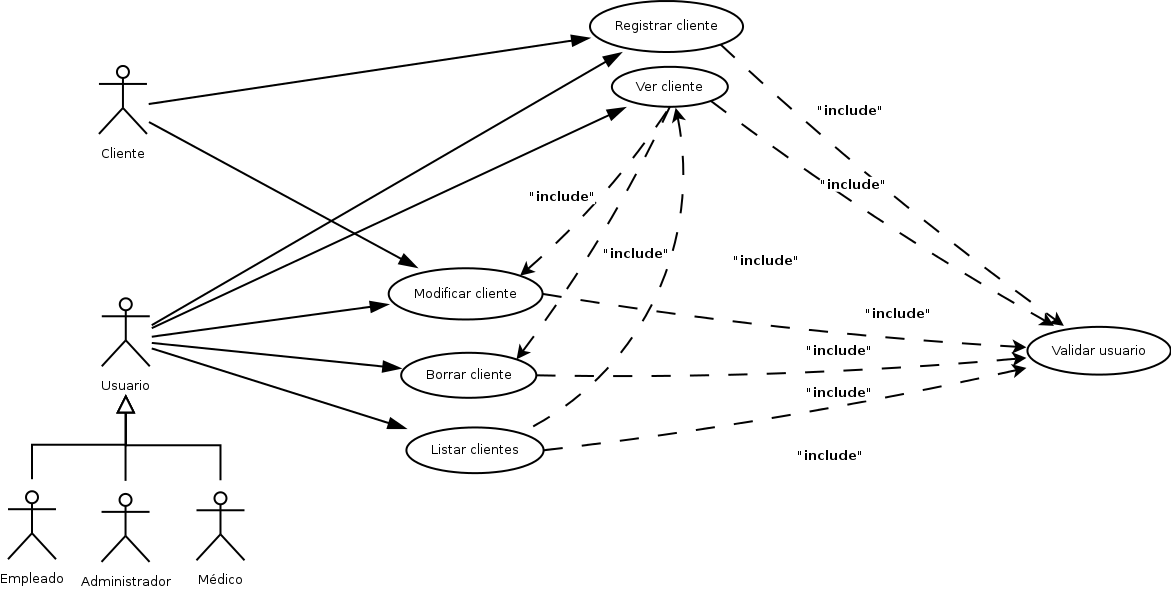
\includegraphics[scale=0.4]{gestionclientes.png}
  \caption{Diagrama caso de uso. Gestión de clientes}
  \label{cu1}
\end{figure}
\smallskip
\hrule height 1pt
\smallskip
\textbf{Caso de uso: Registrar cliente}
\begin{itemize}\renewcommand{\labelitemi}{$\cdot$}
 \item \textbf{Descripción:} El usuario introduce los datos para registrar un nuevo cliente en el sistema.
  \item \textbf{Actores:} Usuario(Principal), Cliente(Secundario)
  \item \textbf{Precondiciones:} Se debe comprobar que el usuario este autenticado en el sistema con el caso de uso Validar usuario.
  \item \textbf{Postcondiciones:} El sistema almacena al nuevo cliente en el sistema.
\end{itemize}
\underline{\textbf{Identificación de escenarios:}}
\begin{itemize}\renewcommand{\labelitemi}{$\circ$}
 \item \textbf{Escenario principal:}
         \begin{enumerate}
          \item El caso de uso se inicia cuando el usuario decide dar de alta un nuevo cliente.
          \item El usuario introduce los datos personales del cliente.
          \item El sistema muestra un mensaje de confirmación.
          \item El usuario pulsa SI en el mensaje de confirmación.
          \item El sistema comprueba que los datos introducidos son correctos y que el cliente no este registrado ya.
	  \item El sistema almacena el cambio del sistema (auditoria).
          \item El cliente queda registrado en el sistema y el sistema muestra un mensaje de éxito.
         \end{enumerate}
  \item \textbf{Escenario alternativos:}\\\\
         4a. El usuario cancela el registro de un nuevo cliente en el sistema.
	      \begin{enumerate}
	       \item El sistema cancela el registro de nuevo cliente en el sistema.
	      \end{enumerate}
	5a. El cliente ya se encuentra registrado en el sistema.
	      \begin{enumerate}
	       \item El sistema muestra el error y pide que se introduzcan nuevos datos.
	      \end{enumerate}
           5b. El usuario introduce de manera incorrecta los datos.
		\begin{enumerate}
		 \item El sistema muestra el error y pide que se introduzcan nuevos datos.
		\end{enumerate}
          *a. El usuario cancela el registro de un nuevo cliente.
\end{itemize}
\smallskip
\hrule height 1pt
\smallskip
\textbf{Caso de uso: Modificar cliente}
\begin{itemize}\renewcommand{\labelitemi}{$\cdot$}
 \item \textbf{Descripción:} El usuario modifica los datos del cliente en el sistema.
  \item \textbf{Actores:} Usuario(Principal), Cliente(Secundario)
  \item \textbf{Precondiciones:} El cliente ya existe en el sistema. Se debe comprobar que el usuario este autenticado en el sistema con el caso de uso Validar usuario.
  \item \textbf{Postcondiciones:} El sistema almacena al cliente con las modificaciones realizadas.
\end{itemize}
\underline{\textbf{Identificación de escenarios:}}
\begin{itemize}\renewcommand{\labelitemi}{$\circ$}
 \item \textbf{Escenario principal:}
         \begin{enumerate}
          \item El caso de uso se inicia cuando el usuario decide modificar un cliente.
          \item El usuario modifica los datos.
          \item El sistema muestra un mensaje de confirmación.
          \item El usuario pulsa SI en el mensaje de confirmación.
	  \item El sistema comprueba los datos introducidos por el usuario.
 	  \item El sistema almacena el cambio del sistema (auditoria).
          \item El sistema guarda los cambios que ha realizado el usuario.
       \end{enumerate}
  \item \textbf{Escenario alternativos:}\\\\
	4a. El usuario cancela la modificación del cliente en el sistema.
	      \begin{enumerate}
	       \item El sistema cancela la modificación del cliente en el sistema.
	      \end{enumerate}
           5a. El usuario modifica de manera incorrecta los datos.
		\begin{enumerate}
		 \item El sistema muestra el error y pide que se introduzcan nuevos datos.
		\end{enumerate}
          *a. El usuario cancela en cualquier momento la modificación de un cliente.
\end{itemize}
\smallskip
\hrule height 1pt
\smallskip
\textbf{Caso de uso: Borrar cliente}
\begin{itemize}\renewcommand{\labelitemi}{$\cdot$}
 \item \textbf{Descripción:} El usuario elimina a un cliente en el sistema.
  \item \textbf{Actores:} Usuario
  \item \textbf{Precondiciones:} El cliente ya existe en el sistema y no tiene operaciones asociadas. Se debe comprobar que el usuario este autenticado en el sistema con el caso de uso Validar usuario.
  \item \textbf{Postcondiciones:} El sistema borra el cliente del sistema.
\end{itemize}
\underline{\textbf{Identificación de escenarios:}}
\begin{itemize}\renewcommand{\labelitemi}{$\circ$}
 \item \textbf{Escenario principal:}
         \begin{enumerate}
          \item El caso de uso se inicia cuando el usuario decide borrar a un cliente.
          \item El sistema muestra un mensaje de confirmación.
          \item El usuario pulsa SI en el mensaje de confirmación.
 	  \item El sistema almacena el cambio del sistema (auditoria).
	  \item El sistema borra al cliente del sistema y muestra un mensaje de éxito.
         \end{enumerate}
  \item \textbf{Escenario alternativos:}\\\\
           3a. El usuario decide no borrar al cliente.
		\begin{enumerate}
		 \item El sistema cancela el proceso de borrado del cliente.
		\end{enumerate}
          *a. El usuario cancela en cualquier momento la eliminación de un cliente.
\end{itemize}

\smallskip
\hrule height 1pt
\smallskip

\textbf{Caso de uso: Ver cliente}
\begin{itemize}\renewcommand{\labelitemi}{$\cdot$}
 \item \textbf{Descripción:} El usuario decide hacer una consulta de un cliente en el sistema.
  \item \textbf{Actores:} Usuario
  \item \textbf{Precondiciones:} El cliente ya existe en el sistema. Se debe comprobar que el usuario este autenticado en el sistema con el caso de uso Validar usuario.
  \item \textbf{Postcondiciones:} El sistema muestra la información del cliente.
\end{itemize}
\underline{\textbf{Identificación de escenarios:}}
\begin{itemize}\renewcommand{\labelitemi}{$\circ$}
 \item \textbf{Escenario principal:}
         \begin{enumerate}
          \item El caso de uso se inicia cuando el usuario decide consultar a un cliente.
	  \item El sistema muestra por pantalla los datos del cliente.
         \end{enumerate}
\end{itemize}
\smallskip
\hrule height 1pt
\smallskip
\textbf{Caso de uso: Listar clientes}
\begin{itemize}\renewcommand{\labelitemi}{$\cdot$}
 \item \textbf{Descripción:} El usuario decide consultar los clientes almacenados en el sistema.
  \item \textbf{Actores:} Usuario
  \item \textbf{Precondiciones:} Se debe comprobar que el usuario este autenticado en el sistema con el caso de uso Validar usuario.
  \item \textbf{Postcondiciones:} El sistema muestra por pantalla todos los clientes.
\end{itemize}
\underline{\textbf{Identificación de escenarios:}}
\begin{itemize}\renewcommand{\labelitemi}{$\circ$}
 \item \textbf{Escenario principal:}
         \begin{enumerate}
          \item El caso de uso se inicia cuando el usuario decide consultar los clientes.
          \item El sistema muestra un listado de los clientes.
          \item El usuario no selecciona un patrón de búsqueda.
          \item El sistema muestra todos los clientes.
         \end{enumerate}
  \item \textbf{Escenario alternativos:}\\
  			3a. El usuario introduce un patrón de búsqueda.
  			\begin{enumerate}
  			\item El sistema muestra los datos acordes a ese patrón de búsqueda.
  			\item El usuario puede seleccionar el patrón de búsqueda cuantas veces desee.
  			\end{enumerate}
          *a. El usuario cancela en cualquier momento la consulta de los clientes.
\end{itemize}

\subsection{Requisito funcional: Gestión productos}

\begin{itemize}
 \item El usuario podrá dar de alta a un determinado producto. 
 \item El usuario podrá consultar e imprimir el listado de todos los productos almacenados en el sistema.
 \item El usuario podrá ver los datos de un producto en concreto.
 \item El usuario podrá modificar los datos de un producto en concreto.
 \item El usuario podrá eliminar un producto del sistema.
 \item El usuario podrá realizar filtrados en los productos.
 \item El usuario podrá dar de alta una determinada familia.
 \item El usuario podrá consultar e imprimir el listado de todas las familias almacenadas en el sistema.
 \item El usuario podrá modificar los datos de una familia en concreto.
 \item El usuario podrá eliminar a una familia del sistema.
 \item El usuario podrá realizar filtrados en las familias.
 \item El usuario podrá realizar movimientos de los productos de una familia a otra.
\item EL usuario podrá ver los productos incluidos en una determinada familia.

\end{itemize}
\begin{figure}[H]
  \centering
    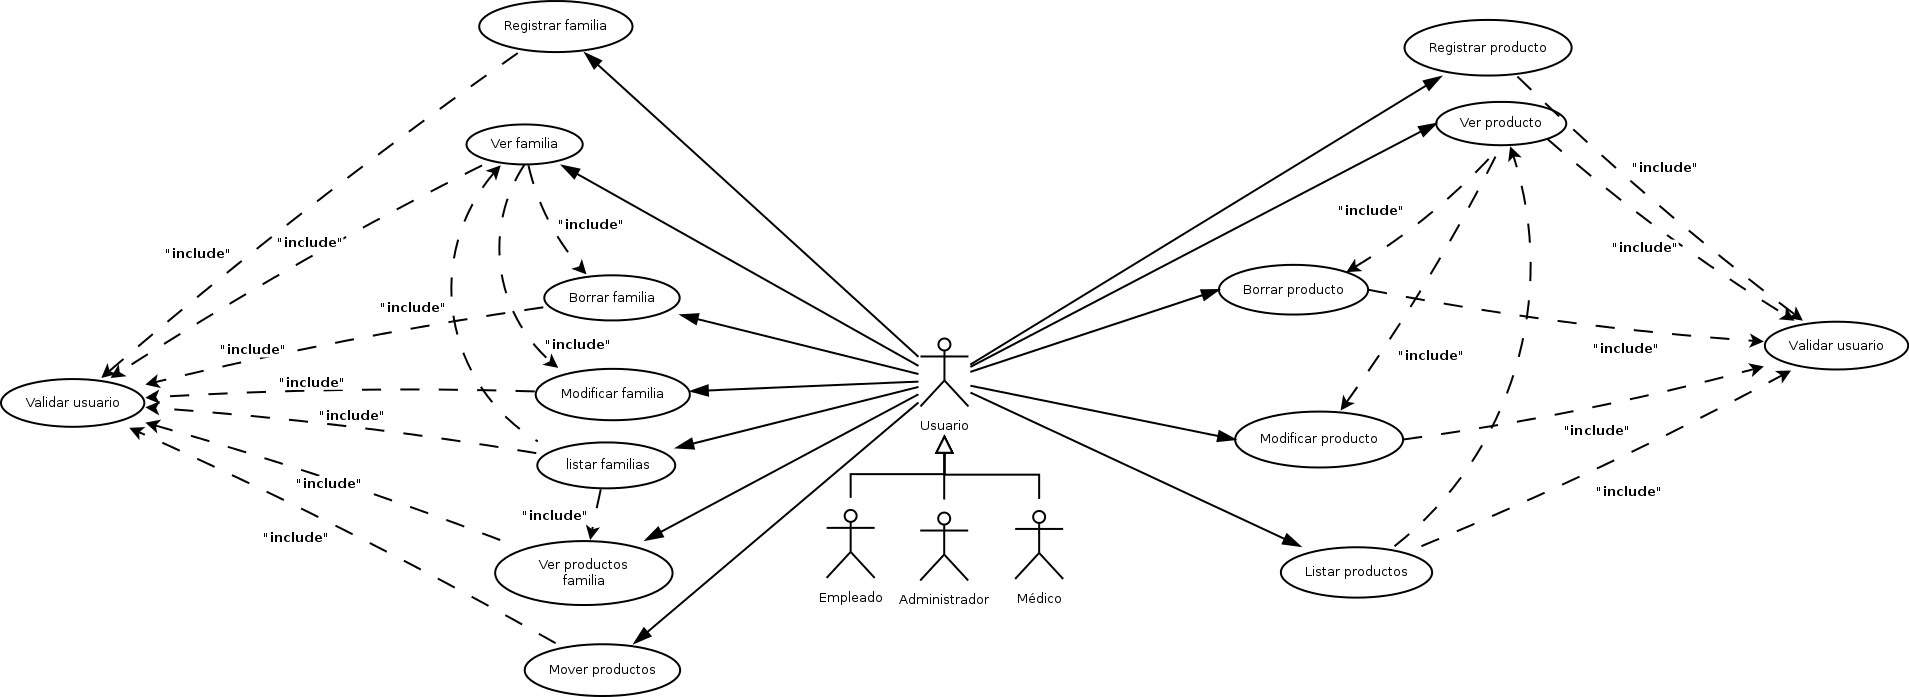
\includegraphics[width=17cm,height=8cm]{gestionproductos.png}
  \caption{Diagrama caso de uso. Gestión de productos}
  \label{cu2}
\end{figure}
\smallskip
\hrule height 1pt
\smallskip
\textbf{Caso de uso: Registrar producto}
\begin{itemize}\renewcommand{\labelitemi}{$\cdot$}
 \item \textbf{Descripción:} El usuario introduce los datos para registrar un nuevo producto en el sistema.
  \item \textbf{Actores:} Usuario
  \item \textbf{Precondiciones:} Se debe comprobar que el usuario este autenticado en el sistema con el caso de uso Validar usuario.
  \item \textbf{Postcondiciones:} El sistema almacena al producto en el sistema.
\end{itemize}
\underline{\textbf{Identificación de escenarios:}}
\begin{itemize}\renewcommand{\labelitemi}{$\circ$}
 \item \textbf{Escenario principal:}
         \begin{enumerate}
          \item El caso de uso se inicia cuando el usuario decide dar de alta un nuevo producto.
          \item El usuario introduce los datos del producto.
	   \item El sistema muestra un mensaje de confirmación.
          \item El usuario pulsa SI en el mensaje de confirmación.
          \item El sistema comprueba que los datos introducidos son correctos y que el producto no este registrado ya.
 	  \item El sistema almacena el cambio del sistema (auditoria).
          \item El producto queda registrado en el sistema y el sistema muestra un mensaje de éxito.
         \end{enumerate}
  \item \textbf{Escenario alternativos:}\\\\
	4a. El usuario decide no registrar un nuevo producto en el sistema.
	      \begin{enumerate}
	       \item El sistema cancela el registro del producto.
	      \end{enumerate}
         5a. El producto ya se encuentra registrado en el sistema.
	      \begin{enumerate}
	       \item El sistema muestra el error y pide que se introduzcan nuevos datos.
	      \end{enumerate}
           5b. El usuario introduce de manera incorrecta los datos.
		\begin{enumerate}
		 \item El sistema muestra el error y pide que se introduzcan nuevos datos.
		\end{enumerate}
          *a. El usuario cancela el registro de un nuevo producto.
\end{itemize}
\smallskip
\hrule height 1pt
\smallskip
\textbf{Caso de uso: Modificar producto}
\begin{itemize}\renewcommand{\labelitemi}{$\cdot$}
 \item \textbf{Descripción:} El usuario modifica los datos de un producto en el sistema.
  \item \textbf{Actores:} Usuario
  \item \textbf{Precondiciones:} El producto ya existe en el sistema. Se debe comprobar que el usuario este autenticado en el sistema con el caso de uso Validar usuario.
  \item \textbf{Postcondiciones:} El usuario almacena el producto con las modificaciones efectuadas en el sistema.
\end{itemize}
\underline{\textbf{Identificación de escenarios:}}
\begin{itemize}\renewcommand{\labelitemi}{$\circ$}
 \item \textbf{Escenario principal:}
         \begin{enumerate}
          \item El caso de uso se inicia cuando el usuario decide modificar un producto.
          \item El usuario modifica los datos del producto.
	  \item El sistema muestra un mensaje de confirmación.
          \item El usuario pulsa SI en el mensaje de confirmación.
          \item El sistema comprueba que los datos introducidos son correctos.
 	  \item El sistema almacena el cambio del sistema (auditoria).
          \item El sistema guarda los cambios que ha realizado el usuario.
         \end{enumerate}
  \item \textbf{Escenario alternativos:}\\\\
	4a. El usuario decide no modificar el producto del sistema.
	      \begin{enumerate}
	       \item El sistema cancela la edición del producto del sistema.
	      \end{enumerate}
           5a. El usuario modifica de manera incorrecta los datos.
		\begin{enumerate}
		 \item El sistema muestra el error y pide que se introduzcan nuevos datos.
		\end{enumerate}
          *a. El usuario cancela en cualquier momento la modificación de un producto.
\end{itemize}
\smallskip
\hrule height 1pt
\smallskip
\textbf{Caso de uso: Borrar producto}
\begin{itemize}\renewcommand{\labelitemi}{$\cdot$}
 \item \textbf{Descripción:} El usuario elimina a un producto en el sistema.
  \item \textbf{Actores:} Usuario
  \item \textbf{Precondiciones:} El producto ya existe en el sistema y no tiene operaciones asociadas. Se debe comprobar que el usuario este autenticado en el sistema con el caso de uso Validar usuario.
  \item \textbf{Postcondiciones:} El sistema borra el producto del sistema.
\end{itemize}
\underline{\textbf{Identificación de escenarios:}}
\begin{itemize}\renewcommand{\labelitemi}{$\circ$}
 \item \textbf{Escenario principal:}
         \begin{enumerate}
          \item El caso de uso se inicia cuando el usuario decide borrar a un producto.
          \item El sistema muestra un mensaje de confirmación.
          \item El usuario pulsa SI en el mensaje de confirmación.
 	  \item El sistema almacena el cambio del sistema (auditoria).
	  \item El sistema borra al producto del sistema y muestra un mensaje de éxito.
         \end{enumerate}
  \item \textbf{Escenario alternativos:}\\\\
           3a. El usuario decide no borrar el producto.
		\begin{enumerate}
		 \item El sistema cancela el proceso de borrado del producto.
		\end{enumerate}
          *a. El usuario cancela en cualquier momento la eliminación de un producto.
\end{itemize}
\smallskip
\hrule height 1pt
\smallskip

\textbf{Caso de uso: Ver producto}
\begin{itemize}\renewcommand{\labelitemi}{$\cdot$}
 \item \textbf{Descripción:} El usuario decide hacer una consulta de un producto en el sistema.
  \item \textbf{Actores:} Usuario
  \item \textbf{Precondiciones:} El producto ya existe en el sistema. Se debe comprobar que el usuario este autenticado en el sistema con el caso de uso Validar usuario.
  \item \textbf{Postcondiciones:} El sistema muestra la información del producto.
\end{itemize}
\underline{\textbf{Identificación de escenarios:}}
\begin{itemize}\renewcommand{\labelitemi}{$\circ$}
 \item \textbf{Escenario principal:}
         \begin{enumerate}
          \item El caso de uso se inicia cuando el usuario decide consultar a un producto del sistema.
	  \item El sistema muestra por pantalla los datos del producto.
         \end{enumerate}
  \item \textbf{Escenario alternativos:}\\\\
          *a. El usuario cancela en cualquier momento la consulta de un producto.
\end{itemize}
\smallskip
\hrule height 1pt
\smallskip
\textbf{Caso de uso: Listar productos}
\begin{itemize}\renewcommand{\labelitemi}{$\cdot$}
 \item \textbf{Descripción:} El usuario consulta los productos almacenados en el sistema.
  \item \textbf{Actores:} usuario
  \item \textbf{Precondiciones:} En el sistema existe al menos un producto. Se debe comprobar que el usuario este autenticado en el sistema con el caso de uso Validar usuario.
  \item \textbf{Postcondiciones:} El sistema muestra por pantalla todos los productos almacenados en el sistema.
\end{itemize}
\underline{\textbf{Identificación de escenarios:}}
\begin{itemize}\renewcommand{\labelitemi}{$\circ$}
 \item \textbf{Escenario principal:}
         \begin{enumerate}
          \item El caso de uso se inicia cuando el usuario decide consultar los productos.
          \item El sistema muestra un listado de los productos.
          \item El usuario no selecciona un patrón de búsqueda.
          \item El sistema muestra todos los productos.
         \end{enumerate}
  \item \textbf{Escenario alternativos:}\\
  			3a. El usuario introduce un patrón de búsqueda.
  			\begin{enumerate}
  			\item El sistema muestra los datos acordes a ese patrón de búsqueda.
  			\item El usuario puede seleccionar el patrón de búsqueda cuantas veces desee.
  			\end{enumerate}
          *a. El usuario cancela en cualquier momento la consulta de los productos.
\end{itemize}
\smallskip
\hrule height 1pt
\smallskip
\textbf{Caso de uso: Registrar familia}
\begin{itemize}\renewcommand{\labelitemi}{$\cdot$}
 \item \textbf{Descripción:} El usuario introduce los datos para registrar una nueva familia en el sistema.
  \item \textbf{Actores:} Usuario
  \item \textbf{Precondiciones:} Se debe comprobar que el usuario este autenticado en el sistema con el caso de uso Validar usuario.
  \item \textbf{Postcondiciones:} El usuario almacena la familia en el sistema.
\end{itemize}
\underline{\textbf{Identificación de escenarios:}}
\begin{itemize}\renewcommand{\labelitemi}{$\circ$}
 \item \textbf{Escenario principal:}
         \begin{enumerate}
          \item El caso de uso se inicia cuando el usuario decide dar de alta una nueva familia.
          \item El usuario introduce los datos de la familia.
	  \item El sistema muestra un mensaje de confirmación.
          \item El usuario pulsa SI en el mensaje de confirmación.
          \item El sistema comprueba que los datos introducidos son correctos y que la familia no este registrada ya.
 	  \item El sistema almacena el cambio del sistema (auditoria).
          \item La familia queda registrada en el sistema y el sistema muestra un mensaje de éxito.
         \end{enumerate}
  \item \textbf{Escenario alternativos:}\\\\
	4a. El usuario decide no registrar una nueva familia en el sistema.
	      \begin{enumerate}
	       \item El sistema cancela el registro de una nueva familia en el sistema.
	      \end{enumerate}
         5a. La familia ya se encuentra registrada en el sistema.
	      \begin{enumerate}
	       \item El sistema muestra el error y pide que se introduzcan nuevos datos.
	      \end{enumerate}
           5b. El usuario introduce de manera incorrecta los datos.
		\begin{enumerate}
		 \item El sistema muestra el error y pide que se introduzcan nuevos datos.
		\end{enumerate}
         *a. El usuario cancela el registro de una nueva familia.
\end{itemize}
\smallskip
\hrule height 1pt
\smallskip
\textbf{Caso de uso: Modificar familia}
\begin{itemize}\renewcommand{\labelitemi}{$\cdot$}
 \item \textbf{Descripción:} El usuario modifica los datos de una familia.
  \item \textbf{Actores:} Usuario
  \item \textbf{Precondiciones:} La familia ya existe en el sistema. Se debe comprobar que el usuario este autenticado en el sistema con el caso de uso Validar usuario.
  \item \textbf{Postcondiciones:} El usuario almacena la familia con las modificaciones efectuadas en el sistema.
\end{itemize}
\underline{\textbf{Identificación de escenarios:}}
\begin{itemize}\renewcommand{\labelitemi}{$\circ$}
 \item \textbf{Escenario principal:}
         \begin{enumerate}
          \item El caso de uso se inicia cuando el usuario decide modificar una familia.
          \item El usuario modifica los datos de la familia.
	  \item El sistema muestra un mensaje de confirmación.
          \item El usuario pulsa SI en el mensaje de confirmación.
          \item El sistema comprueba que los datos introducidos sean correctos.
 	  \item El sistema almacena el cambio del sistema (auditoria).
          \item El sistema guarda los cambios que ha realizado el usuario.
         \end{enumerate}
  \item \textbf{Escenario alternativos:}\\\\	
	4a. El usuario decide no modificar la familia del sistema.
	      \begin{enumerate}
	       \item El sistema cancela la edición de la familia en el sistema.
	      \end{enumerate}
           5a. El usuario modifica de manera incorrecta los datos.
		\begin{enumerate}
		 \item El sistema muestra el error y pide que se introduzcan nuevos datos.
		\end{enumerate}
          *a. El usuario cancela en cualquier momento la modificación de una familia.
\end{itemize}
\smallskip
\hrule height 1pt
\smallskip
\textbf{Caso de uso: Borrar familia}
\begin{itemize}\renewcommand{\labelitemi}{$\cdot$}
 \item \textbf{Descripción:} El usuario elimina a una familia en el sistema.
  \item \textbf{Actores:} usuario
  \item \textbf{Precondiciones:} La familia ya existe en el sistema. Se debe comprobar que el usuario este autenticado en el sistema con el caso de uso Validar usuario.
  \item \textbf{Postcondiciones:} El sistema borra la familia del sistema.
\end{itemize}
\underline{\textbf{Identificación de escenarios:}}
\begin{itemize}\renewcommand{\labelitemi}{$\circ$}
 \item \textbf{Escenario principal:}
         \begin{enumerate}
          \item El caso de uso se inicia cuando el usuario decide borrar a una familia.
          \item El sistema muestra un mensaje de confirmación.
          \item El usuario pulsa SI en el mensaje de confirmación.
 	  \item El sistema almacena el cambio del sistema (auditoria).
	   \item El sistema deja los productos sin familia, se borra la familia del sistema y muestra un mensaje de éxito.
         \end{enumerate}
  \item \textbf{Escenario alternativos:}\\\\
	3a. El usuario decide no borrar la familia.
		\begin{enumerate}
		 \item El sistema cancela el proceso de borrado de la familia.
		\end{enumerate}
          *a. El usuario cancela en cualquier momento la eliminación de la familia.
\end{itemize}

\smallskip
\hrule height 1pt
\smallskip
\textbf{Caso de uso: Ver familia}
\begin{itemize}\renewcommand{\labelitemi}{$\cdot$}
 \item \textbf{Descripción:} El usuario decide hacer una consulta de una familia en el sistema.
  \item \textbf{Actores:} usuario
  \item \textbf{Precondiciones:} La familia ya existe en el sistema. Se debe comprobar que el usuario este autenticado en el sistema con el caso de uso Validar usuario.
  \item \textbf{Postcondiciones:} El sistema muestra la información de la familia por pantalla.
\end{itemize}
\underline{\textbf{Identificación de escenarios:}}
\begin{itemize}\renewcommand{\labelitemi}{$\circ$}
 \item \textbf{Escenario principal:}
         \begin{enumerate}
          \item El caso de uso se inicia cuando el usuario decide consultar a una familia del sistema.
	  \item El sistema muestra por pantalla los datos de la familia.
         \end{enumerate}
  \item \textbf{Escenario alternativos:}\\\\
          *a. El usuario cancela en cualquier momento la consulta de una familia.
\end{itemize}
\smallskip
\hrule height 1pt
\smallskip
\textbf{Caso de uso: Listar familias}
\begin{itemize}\renewcommand{\labelitemi}{$\cdot$}
 \item \textbf{Descripción:} El usuario consulta las familias almacenadas en el sistema.
  \item \textbf{Actores:} usuario
  \item \textbf{Precondiciones:} En el sistema existe al menos una familia. Se debe comprobar que el usuario este autenticado en el sistema con el caso de uso Validar usuario.
  \item \textbf{Postcondiciones:} El sistema muestra por pantalla todas las familias almacenadas en el sistema.
\end{itemize}
\underline{\textbf{Identificación de escenarios:}}
\begin{itemize}\renewcommand{\labelitemi}{$\circ$}
 \item \textbf{Escenario principal:}
         \begin{enumerate}
          \item El caso de uso se inicia cuando el usuario decide consultar las familias.
          \item El sistema muestra un listado de las familias.
          \item El usuario no selecciona un patrón de búsqueda.
          \item El sistema muestra todas las familias.
         \end{enumerate}
  \item \textbf{Escenario alternativos:}\\
  			3a. El usuario introduce un patrón de búsqueda.
  			\begin{enumerate}
  			\item El sistema muestra los datos acordes a ese patrón de búsqueda.
  			\item El usuario puede seleccionar el patrón de búsqueda cuantas veces desee.
  			\end{enumerate}
          *a. El usuario cancela en cualquier momento la consulta de las familias.
\end{itemize}
\smallskip
\hrule height 1pt
\smallskip
\textbf{Caso de uso: Mover productos}
\begin{itemize}\renewcommand{\labelitemi}{$\cdot$}
 \item \textbf{Descripción:} El usuario mueve los productos entre las familias del sistema.
  \item \textbf{Actores:} Usuario
  \item \textbf{Precondiciones:} Se debe comprobar que el usuario este autenticado en el sistema con el caso de uso Validar usuario.
  \item \textbf{Postcondiciones:} El sistema cambia de familia a los productos deseados por el usuario.
\end{itemize}
\underline{\textbf{Identificación de escenarios:}}
\begin{itemize}\renewcommand{\labelitemi}{$\circ$}
 \item \textbf{Escenario principal:}
         \begin{enumerate}
          \item El caso de uso se inicia cuando el usuario decide mover productos.
          \item El sistema muestra dos cajas para poder mover productos entre familias.
          \item El usuario selecciona las familias afectadas.
          \item El usuario arrastra los productos de una familia a otra.
 	  \item El sistema almacena el cambio del sistema (auditoria).
          \item El sistema guarda los cambios.
         \end{enumerate}
  \item \textbf{Escenario alternativos:}\\
  	   3a. El usuario puede seleccionar las familias afectadas y productos cuantas veces desee.\\
           *a. El usuario cancela en cualquier momento el movimiento de productos.
\end{itemize}

\subsection{Requisito funcional: Gestión proveedores}

\begin{itemize}
 \item El usuario podrá dar de alta a un determinado proveedor. 
 \item El usuario podrá consultar e imprimir el listado de todos los proveedores almacenados en el sistema.
 \item El usuario podrá ver los datos de un proveedor en concreto.
 \item El usuario podrá modificar los datos de un proveedor en concreto.
 \item El usuario podrá eliminar a un proveedor del sistema.
 \item El usuario podrá realizar filtrados de los proveedores.
\item El usuario podrá ver los productos suministrados por un determinado proveedor.
\end{itemize}
\begin{figure}[H]
  \centering
    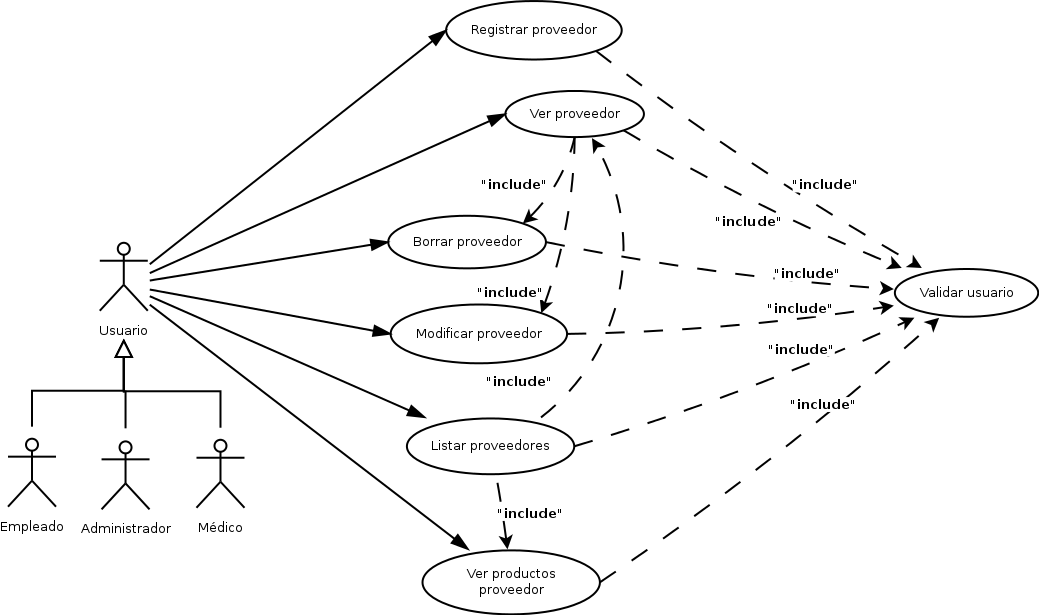
\includegraphics[width=12cm,height=8cm]{gestionproveedores.png}
  \caption{Diagrama caso de uso. Gestión de proveedores}
  \label{cu3}
\end{figure}
\smallskip
\hrule height 1pt
\smallskip
\textbf{Caso de uso: Registrar proveedor}
\begin{itemize}\renewcommand{\labelitemi}{$\cdot$}
 \item \textbf{Descripción:} El usuario introduce los datos para registrar un nuevo proveedor en el sistema.
  \item \textbf{Actores:} Usuario
  \item \textbf{Precondiciones:} Se debe comprobar que el usuario este autenticado en el sistema con el caso de uso Validar usuario.
  \item \textbf{Postcondiciones:} El usuario almacena al proveedor en el sistema.
\end{itemize}
\underline{\textbf{Identificación de escenarios:}}
\begin{itemize}\renewcommand{\labelitemi}{$\circ$}
 \item \textbf{Escenario principal:}
         \begin{enumerate}
          \item El caso de uso se inicia cuando el usuario decide dar de alta un nuevo proveedor.
          \item El usuario introduce los datos del proveedor.
          \item El sistema muestra un mensaje de confirmación.
          \item El usuario pulsa SI en el mensaje de confirmación.
          \item El sistema comprueba que los datos introducidos son correctos y que el proveedor no este registrado ya.
 	  \item El sistema almacena el cambio del sistema (auditoria).
          \item El proveedor queda registrado en el sistema y el sistema muestra un mensaje de éxito.
         \end{enumerate}
  \item \textbf{Escenario alternativos:}\\\\
	4a. El usuario decide no registrar un nuevo proveedor en el sistema.
	      \begin{enumerate}
	       \item El sistema cancela el registro de un nuevo proveedor en el sistema.
	      \end{enumerate}
         5a. El proveedor ya se encuentra registrado en el sistema.
	      \begin{enumerate}
	       \item El sistema muestra el error y pide que se introduzcan nuevos datos.
	      \end{enumerate}
           5b. El usuario introduce de manera incorrecta los datos.
		\begin{enumerate}
		 \item El sistema muestra el error y pide que se introduzcan nuevos datos.
		\end{enumerate}
          *a. El usuario cancela el registro de un nuevo proveedor.
\end{itemize}
\smallskip
\hrule height 1pt
\smallskip
\textbf{Caso de uso: Editar proveedor}
\begin{itemize}\renewcommand{\labelitemi}{$\cdot$}
 \item \textbf{Descripción:} El usuario modifica los datos del proveedor en el sistema.
  \item \textbf{Actores:} Usuario
  \item \textbf{Precondiciones:} El proveedor ya existe en el sistema. Se debe comprobar que el usuario este autenticado en el sistema con el caso de uso Validar usuario.
  \item \textbf{Postcondiciones:} El usuario almacena al proveedor con las modificaciones efectuadas en el sistema.
\end{itemize}
\underline{\textbf{Identificación de escenarios:}}
\begin{itemize}\renewcommand{\labelitemi}{$\circ$}
 \item \textbf{Escenario principal:}
         \begin{enumerate}
          \item El caso de uso se inicia cuando el usuario decide modificar un proveedor.
          \item El usuario modifica los datos.
          \item El sistema muestra un mensaje de confirmación.
          \item El usuario pulsa SI en el mensaje de confirmación.
          \item El sistema comprueba que los datos introducidos son correctos.
 	  \item El sistema almacena el cambio del sistema (auditoria).
          \item El sistema guarda los cambios que ha realizado el usuario.
         \end{enumerate}
  \item \textbf{Escenario alternativos:}\\\\
	4a. El usuario decide no editar al proveedor.
	      \begin{enumerate}
	       \item El sistema cancela la edición del proveedor en el sistema.
	      \end{enumerate}
           5a. El usuario modifica de manera incorrecta los datos.
		\begin{enumerate}
		 \item El sistema muestra el error y pide que se introduzcan nuevos datos.
		\end{enumerate}
          *a. El usuario cancela en cualquier momento la edición de un proveedor.
\end{itemize}
\smallskip
\hrule height 1pt
\smallskip
\textbf{Caso de uso: Borrar proveedor}
\begin{itemize}\renewcommand{\labelitemi}{$\cdot$}
 \item \textbf{Descripción:} El usuario elimina a un proveedor en el sistema.
  \item \textbf{Actores:} Usuario
  \item \textbf{Precondiciones:} El proveedor ya existe en el sistema. Se debe comprobar que el usuario este autenticado en el sistema con el caso de uso Validar usuario.
  \item \textbf{Postcondiciones:} El sistema borra al proveedor del sistema.
\end{itemize}
\underline{\textbf{Identificación de escenarios:}}
\begin{itemize}\renewcommand{\labelitemi}{$\circ$}
 \item \textbf{Escenario principal:}
         \begin{enumerate}
          \item El caso de uso se inicia cuando el usuario decide borrar a un proveedor.
          \item El sistema muestra un mensaje de confirmación.
          \item El usuario pulsa SI en el mensaje de confirmación.
 	  \item El sistema almacena el cambio del sistema (auditoria).
	      \item El sistema borra al proveedor del sistema y muestra un mensaje de éxito.
         \end{enumerate}
  \item \textbf{Escenario alternativos:}\\\\
           3a. El usuario decide no borrar al proveedor.
		\begin{enumerate}
		 \item El sistema cancela el proceso de borrado del proveedor.
		\end{enumerate}
          *a. El usuario cancela en cualquier momento la eliminación de un proveedor.
\end{itemize}
\smallskip
\hrule height 1pt
\smallskip

\textbf{Caso de uso: Ver proveedor}
\begin{itemize}\renewcommand{\labelitemi}{$\cdot$}
 \item \textbf{Descripción:} El usuario decide hacer una consulta de un proveedor en el sistema.
  \item \textbf{Actores:} usuario
  \item \textbf{Precondiciones:} El proveedor ya existe en el sistema. Se debe comprobar que el usuario este autenticado en el sistema con el caso de uso Validar usuario.
  \item \textbf{Postcondiciones:} El sistema muestra la información del proveedor.
\end{itemize}
\underline{\textbf{Identificación de escenarios:}}
\begin{itemize}\renewcommand{\labelitemi}{$\circ$}
 \item \textbf{Escenario principal:}
         \begin{enumerate}
          \item El caso de uso se inicia cuando el usuario decide consultar a un proveedor.
	  \item El sistema muestra por pantalla los datos del proveedor.
         \end{enumerate}
\end{itemize}
\smallskip
\hrule height 1pt
\smallskip
\textbf{Caso de uso: Listar proveedores}
\begin{itemize}\renewcommand{\labelitemi}{$\cdot$}
 \item \textbf{Descripción:} El usuario consulta los proveedores almacenados en el sistema.
  \item \textbf{Actores:} usuario
  \item \textbf{Precondiciones:} En el sistema existe al menos un proveedor. Se debe comprobar que el usuario este autenticado en el sistema con el caso de uso Validar usuario.
  \item \textbf{Postcondiciones:} El sistema muestra por pantalla todos los proveedores.
\end{itemize}
\underline{\textbf{Identificación de escenarios:}}
\begin{itemize}\renewcommand{\labelitemi}{$\circ$}
 \item \textbf{Escenario principal:}
         \begin{enumerate}
          \item El caso de uso se inicia cuando el usuario decide consultar los proveedores.
          \item El sistema muestra un listado de los proveedores.
          \item El usuario no selecciona un patrón de búsqueda.
          \item El sistema muestra todos los proveedores.
         \end{enumerate}
  \item \textbf{Escenario alternativos:}\\
  			3a. El usuario introduce un patrón de búsqueda.
  			\begin{enumerate}
  			\item El sistema muestra los datos acordes a ese patrón de búsqueda.
  			\item El usuario puede seleccionar el patrón de búsqueda cuantas veces desee.
  			\end{enumerate}
          *a. El usuario cancela en cualquier momento la consulta de los proveedores.
\end{itemize}

\subsection{Requisito funcional: Gestión usuarios}

\begin{itemize}
 \item El administrador podrá dar de alta a un determinado usuario. El usuario se identificará por su DNI. 
 \item El administrador podrá consultar e imprimir el listado de todos los usuarios almacenados en el sistema.
 \item El administrador podrá ver los datos de un usuario en concreto.
 \item El administrador podrá modificar los datos de un usuario en concreto.
 \item El administrador podrá desactivar a un usuario del sistema.
 \item El administrador podrá realizar filtrados de los usuarios del sistema.

\end{itemize}
\begin{figure}[H]
  \centering
    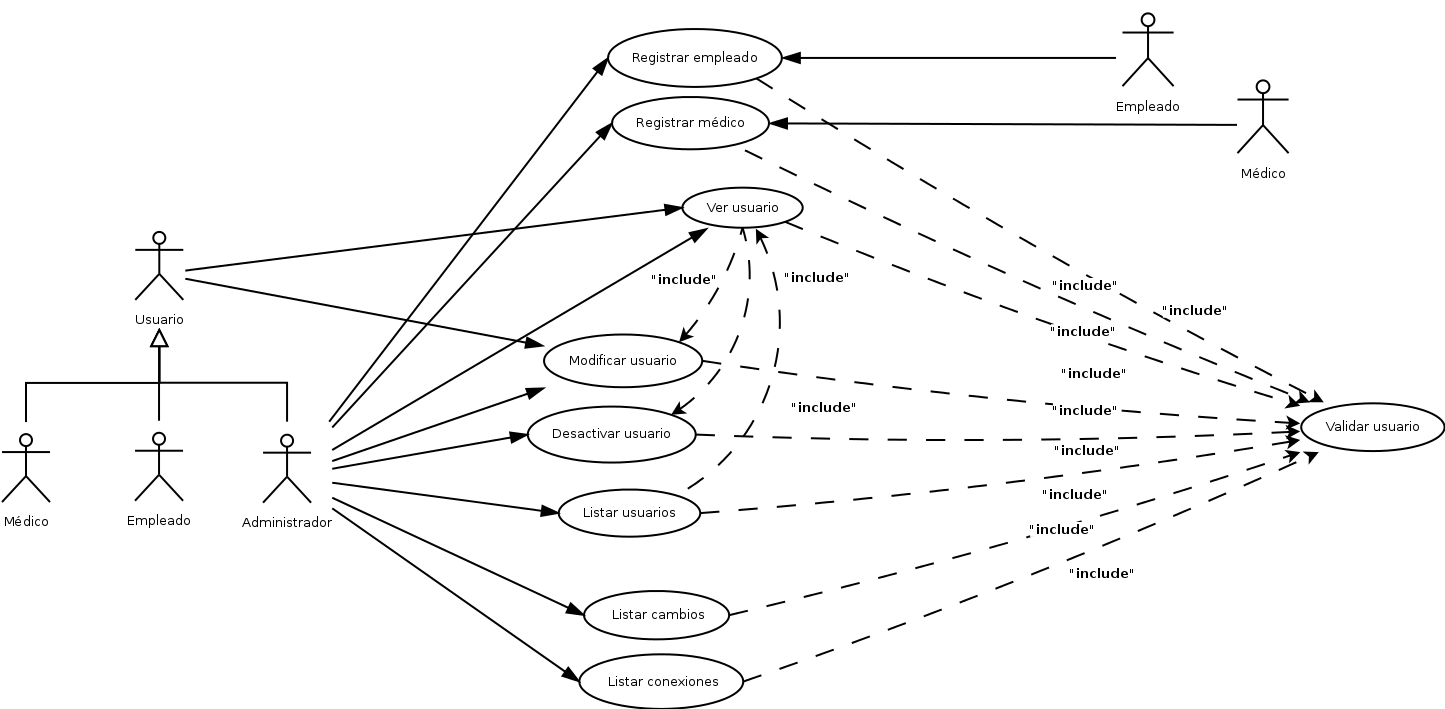
\includegraphics[width=12cm,height=8cm]{gestionempledos.png}
  \caption{Diagrama caso de uso. Gestión de usuarios}
  \label{cu4}
\end{figure}
\smallskip
\hrule height 1pt
\smallskip
\textbf{Caso de uso: Registrar empleado}
\begin{itemize}\renewcommand{\labelitemi}{$\cdot$}
 \item \textbf{Descripción:} El administrador introduce los datos para registrar un nuevo empleado en el sistema.
  \item \textbf{Actores:} Administrador
  \item \textbf{Precondiciones:} Se debe comprobar que el administrador este autenticado en el sistema con el caso de uso Validar usuario.
  \item \textbf{Postcondiciones:} El administrador almacena al empleado en el sistema.
\end{itemize}
\underline{\textbf{Identificación de escenarios:}}
\begin{itemize}\renewcommand{\labelitemi}{$\circ$}
 \item \textbf{Escenario principal:}
         \begin{enumerate}
          \item El caso de uso se inicia cuando el administrador decide dar de alta un nuevo empleado.
          \item El administrador introduce los datos del empleado.
  	  \item El sistema muestra un mensaje de confirmación.
          \item El administrador pulsa SI en el mensaje de confirmación.
          \item El sistema comprueba que los datos introducidos son correctos y que el empleado no este registrado ya.
       	  \item El sistema manda un email con la contraseña al nuevo empleado.
 	  \item El sistema almacena el cambio del sistema (auditoria).
          \item El empleado queda registrado en el sistema y el sistema muestra un mensaje de éxito.
         \end{enumerate}
  \item \textbf{Escenario alternativos:}\\\\
	4a. El administrador decide no registrar a un nuevo empleado.
	      \begin{enumerate}
	       \item El sistema cancela el registro de un nuevo empleado en el sistema.
	      \end{enumerate}
         5a. El empleado ya se encuentra registrado en el sistema.
	      \begin{enumerate}
	       \item El sistema muestra el error y pide que se introduzcan nuevos datos.
	      \end{enumerate}
           5b. El administrador introduce de manera incorrecta los datos.
		\begin{enumerate}
		 \item El sistema muestra el error y pide que se introduzcan nuevos datos.
		\end{enumerate}
          *a. El administrador cancela el registro de un nuevo empleado.
\end{itemize}
\smallskip
\hrule height 1pt
\smallskip
\textbf{Caso de uso: Registrar médico}
\begin{itemize}\renewcommand{\labelitemi}{$\cdot$}
 \item \textbf{Descripción:} El administrador introduce los datos para registrar un nuevo médico en el sistema.
  \item \textbf{Actores:} Administrador
  \item \textbf{Precondiciones:} Se debe comprobar que el administrador este autenticado en el sistema con el caso de uso Validar usuario.
  \item \textbf{Postcondiciones:} El administrador almacena al médico en el sistema.
\end{itemize}
\underline{\textbf{Identificación de escenarios:}}
\begin{itemize}\renewcommand{\labelitemi}{$\circ$}
 \item \textbf{Escenario principal:}
         \begin{enumerate}
          \item El caso de uso se inicia cuando el administrador decide dar de alta un nuevo médico.
          \item El usuario introduce los datos del médico.
  	  \item El sistema muestra un mensaje de confirmación.
          \item El administrador pulsa SI en el mensaje de confirmación.
          \item El sistema comprueba que los datos introducidos son correctos y que el médico no este registrado ya.
	\item El sistema manda un email con la contraseña al nuevo usuario.
 	  \item El sistema almacena el cambio del sistema (auditoria).
          \item El médico queda registrado en el sistema y el sistema muestra un mensaje de éxito.
         \end{enumerate}
  \item \textbf{Escenario alternativos:}\\\\
	4a. El administrador decide no registrar a un nuevo médico.
	      \begin{enumerate}
	       \item El sistema cancela el registro de un nuevo médico en el sistema.
	      \end{enumerate}
         5a. El médico ya se encuentra registrado en el sistema.
	      \begin{enumerate}
	       \item El sistema muestra el error y pide que se introduzcan nuevos datos.
	      \end{enumerate}
           5b. El administrador introduce de manera incorrecta los datos.
		\begin{enumerate}
		 \item El sistema muestra el error y pide que se introduzcan nuevos datos.
		\end{enumerate}
          *a. El administrador cancela el registro de un nuevo médico.
\end{itemize}
\smallskip
\hrule height 1pt
\smallskip
\textbf{Caso de uso: Modificar empleado}
\begin{itemize}\renewcommand{\labelitemi}{$\cdot$}
 \item \textbf{Descripción:} El administrador modifica los datos de un empleado en el sistema.
  \item \textbf{Actores:} Administrador, Usuario
  \item \textbf{Precondiciones:} El empleado ya existe en el sistema. Se debe comprobar que el administrador este autenticado en el sistema con el caso de uso Validar usuario. Si el usuario no es administrador sólo podrá modificar sus propios datos.
  \item \textbf{Postcondiciones:} El administrador almacena al empleado con las modificaciones efectuadas en el sistema.
\end{itemize}
\underline{\textbf{Identificación de escenarios:}}
\begin{itemize}\renewcommand{\labelitemi}{$\circ$}
 \item \textbf{Escenario principal:}
         \begin{enumerate}
          \item El caso de uso se inicia cuando el administrador decide modificar un empleado.
          \item El administrador modifica los datos.
  	  \item El sistema muestra un mensaje de confirmación.
          \item El usuario pulsa SI en el mensaje de confirmación.
          \item El sistema comprueba que los datos introducidos son correctos.
 	  \item El sistema almacena el cambio del sistema (auditoria).
          \item El sistema guarda los cambios que ha realizado el administrador.
         \end{enumerate}
  \item \textbf{Escenario alternativos:}\\\\
	   4a. El administrador decide no editar al empleado.
	      \begin{enumerate}
	       \item El sistema cancela la edición de un empleado en el sistema.
	      \end{enumerate}
           5a. El administrador modifica de manera incorrecta los datos.
		\begin{enumerate}
		 \item El sistema muestra el error y pide que se introduzcan nuevos datos.
		\end{enumerate}
          *a. El administrador cancela en cualquier momento la edición de un empleado.
\end{itemize}
\smallskip
\hrule height 1pt
\smallskip

\textbf{Caso de uso: Desactivar empleado}
\begin{itemize}\renewcommand{\labelitemi}{$\cdot$}
 \item \textbf{Descripción:} El administrador desactiva a un empleado en el sistema.
  \item \textbf{Actores:} Administrador
  \item \textbf{Precondiciones:} El empleado ya existe en el sistema. Se debe comprobar que el administrador este autenticado en el sistema con el caso de uso Validar usuario.
  \item \textbf{Postcondiciones:} El sistema desactiva al empleado del sistema.
\end{itemize}
\underline{\textbf{Identificación de escenarios:}}
\begin{itemize}\renewcommand{\labelitemi}{$\circ$}
 \item \textbf{Escenario principal:}
         \begin{enumerate}
          \item El caso de uso se inicia cuando el administrador decide desactivar a un empleado.
          \item El sistema muestra un mensaje de confirmación.
          \item El administrador pulsa SI en el mensaje de confirmación.
 	  \item El sistema almacena el cambio del sistema (auditoria).
	   \item El sistema desactiva al usuario del sistema y muestra un mensaje de éxito.
         \end{enumerate}
  \item \textbf{Escenario alternativos:}\\\\
           3a. El administrador decide no desactivar al usuario.
		\begin{enumerate}
		 \item El sistema cancela el proceso de desactivación del usuario.
		\end{enumerate}
          *a. El administrador cancela en cualquier momento la desactivación de un usuario.
\end{itemize}
\smallskip
\hrule height 1pt
\smallskip
\textbf{Caso de uso: Ver empleado}
\begin{itemize}\renewcommand{\labelitemi}{$\cdot$}
 \item \textbf{Descripción:} El administrador decide hacer una consulta de un empleado en el sistema.
  \item \textbf{Actores:} Administrador, Usuario
  \item \textbf{Precondiciones:} El empleado ya existe en el sistema. Se debe comprobar que el empleado este autenticado en el sistema con el caso de uso Validar usuario. Si el usuario no es administrador sólo podrá ver sus propios datos.
  \item \textbf{Postcondiciones:} El sistema muestra la información del empleado.
\end{itemize}
\underline{\textbf{Identificación de escenarios:}}
\begin{itemize}\renewcommand{\labelitemi}{$\circ$}
 \item \textbf{Escenario principal:}
         \begin{enumerate}
          \item El caso de uso se inicia cuando el administrador decide consultar a un empleado.
	  \item El sistema muestra por pantalla los datos del empleado.
         \end{enumerate}
\end{itemize}
\smallskip
\hrule height 1pt
\smallskip
\textbf{Caso de uso: Listar usuarios}
\begin{itemize}\renewcommand{\labelitemi}{$\cdot$}
 \item \textbf{Descripción:} El administrador consulta los usuarios almacenados en el sistema.
  \item \textbf{Actores:} Administrador
  \item \textbf{Precondiciones:} Se debe comprobar que el administrador este autenticado en el sistema con el caso de uso Validar usuario.
  \item \textbf{Postcondiciones:} El sistema muestra por pantalla todos los usuarios.
\end{itemize}
\underline{\textbf{Identificación de escenarios:}}
\begin{itemize}\renewcommand{\labelitemi}{$\circ$}
 \item \textbf{Escenario principal:}
         \begin{enumerate}
          \item El caso de uso se inicia cuando el administrador decide consultar los usuarios.
          \item El sistema muestra un listado de los usuarios.
          \item El administrador no selecciona un patrón de búsqueda.
          \item El sistema muestra todos los usuarios.
         \end{enumerate}
  \item \textbf{Escenario alternativos:}\\
  			3a. El administrador introduce un patrón de búsqueda.
  			\begin{enumerate}
  			\item El sistema muestra los datos acordes a ese patrón de búsqueda.
  			\item El usuario puede seleccionar el patrón de búsqueda cuantas veces desee.
  			\end{enumerate}
          *a. El administrador cancela en cualquier momento la consulta de los usuarios.
\end{itemize}

\smallskip
\hrule height 1pt
\smallskip
\textbf{Caso de uso: Listar cambios}
\begin{itemize}\renewcommand{\labelitemi}{$\cdot$}
 \item \textbf{Descripción:} El administrador consulta los cambios que se han efectuado en el sistema.
  \item \textbf{Actores:} Administrador
  \item \textbf{Precondiciones:} Se debe comprobar que el administrador este autenticado en el sistema con el caso de uso Validar usuario.
  \item \textbf{Postcondiciones:} El sistema muestra por pantalla todos los cambios del sistema.
\end{itemize}
\underline{\textbf{Identificación de escenarios:}}
\begin{itemize}\renewcommand{\labelitemi}{$\circ$}
 \item \textbf{Escenario principal:}
         \begin{enumerate}
          \item El caso de uso se inicia cuando el administrador decide consultar los cambios del sistema.
          \item El sistema muestra por pantalla los cambios que han efectuado los usuarios.
         \end{enumerate}
          *a. El administrador cancela en cualquier momento la consulta de los cambios efectuados por los usuarios.
\end{itemize}

\smallskip
\hrule height 1pt
\smallskip
\textbf{Caso de uso: Listar conexiones}
\begin{itemize}\renewcommand{\labelitemi}{$\cdot$}
 \item \textbf{Descripción:} El administrador consulta las conexiones que se han efectuado al sistema.
  \item \textbf{Actores:} Administrador
  \item \textbf{Precondiciones:} Se debe comprobar que el administrador este autenticado en el sistema con el caso de uso Validar usuario.
  \item \textbf{Postcondiciones:} El sistema muestra por pantalla todas las conexiones de los usuarios de la aplicación al sistema.
\end{itemize}
\underline{\textbf{Identificación de escenarios:}}
\begin{itemize}\renewcommand{\labelitemi}{$\circ$}
 \item \textbf{Escenario principal:}
         \begin{enumerate}
          \item El caso de uso se inicia cuando el administrador decide consultar las conexiones al sistema.
          \item El sistema muestra por pantalla las conexiones al sistema de los usuarios.
         \end{enumerate}
          *a. El administrador cancela en cualquier momento la consulta de las conexiones al sistema.
\end{itemize}


\subsection{Requisito funcional: Gestión ventas}

\begin{itemize}
 \item El usuario podrá crear una nueva venta en el sistema.
 \item El usuario podrá consultar e imprimir el listado de todas las ventas del sistema.
 \item El usuario podrá ver los productos asociados a una venta.
 \item El usuario podrá consultar los productos si la venta tiene algún apartado, reserva o devolución.
 \item El usuario podrá realizar filtrados de las ventas del sistema.
 \item El usuario podrá generar documentos de las ventas.

\end{itemize}
\begin{figure}[H]
  \centering
    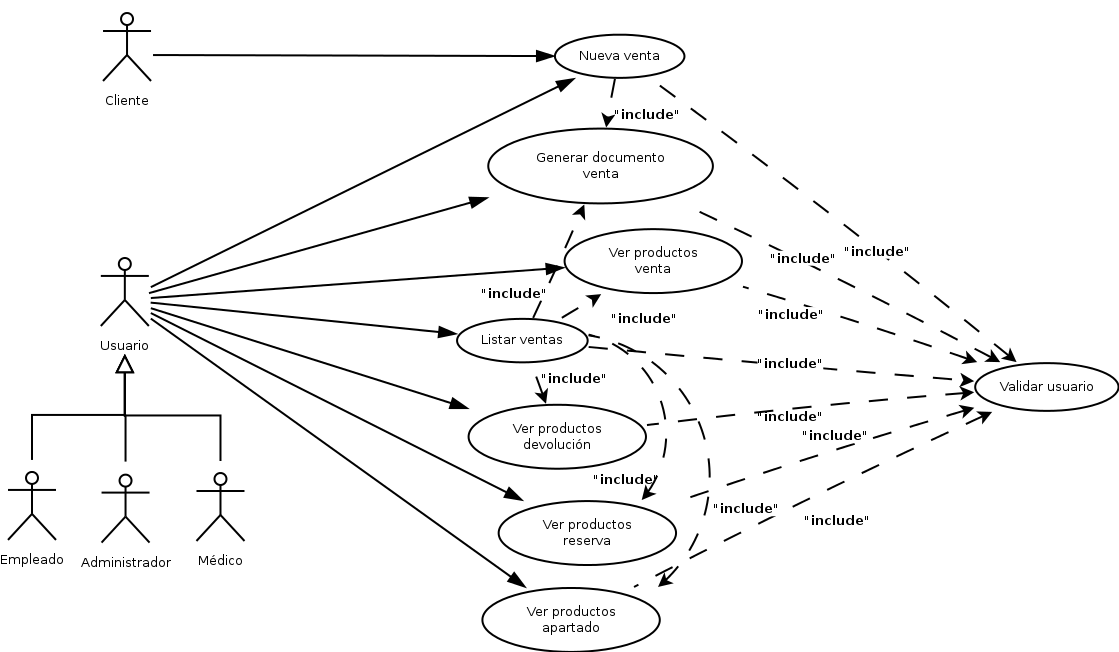
\includegraphics[scale=0.4]{gestionventas.png}
  \caption{Diagrama caso de uso. Gestión ventas}
  \label{cu7}
\end{figure}
\smallskip
\hrule height 1pt
\smallskip
\textbf{Caso de uso: Nueva venta}
\begin{itemize}\renewcommand{\labelitemi}{$\cdot$}
  \item \textbf{Descripción:} El usuario introduce los datos para registrar una nueva venta en el sistema.
  \item \textbf{Actores:} Usuario(Principal), Cliente (Secundario)
  \item \textbf{Precondiciones:} Se debe comprobar que el usuario este autenticado en el sistema con el caso de uso Validar usuario.
  \item \textbf{Postcondiciones:} El usuario almacena la venta en el sistema.
\end{itemize}
\underline{\textbf{Identificación de escenarios:}}
\begin{itemize}\renewcommand{\labelitemi}{$\circ$}
 \item \textbf{Escenario principal:}
         \begin{enumerate}
          \item El caso de uso se inicia cuando el usuario decide crear una nueva venta.
 	 \item El sistema muestra por pantalla todos los clientes para que se puedan seleccionar.
	\item El usuario selecciona el cliente al que quiere realizar la venta.
          \item El sistema muestra por pantalla todos los productos para que se puedan seleccionar.
          \item El usuario introduce los productos y cantidades que desea introducir en la venta.
          \item El sistema comprueba que los datos introducidos son correctos.
	  \item El usuario introduce la forma de pago tarjeta.
  	  \item El sistema muestra un mensaje de confirmación.
          \item El usuario pulsa SI en el mensaje de confirmación.
	  \item El sistema actualiza los stocks de los productos.
 	  \item El sistema almacena el cambio del sistema (auditoria).
          \item La venta queda almacenada en el sistema y se muestra un mensaje de éxito.
         \end{enumerate}
  \item \textbf{Escenario alternativos:}\\\\
	  6a. El usuario introduce de manera incorrecta los datos.
		\begin{enumerate}
		 \item El sistema muestra el error y pide que se introduzcan nuevos datos.
		\end{enumerate}
	7a. El usuario elige el pago con efectivo.
		\begin{enumerate}
		\item El usuario introduce el dinero entregado por el cliente.
		
		 \item El sistema mostrará en el mensaje de confirmación el cambio a devolver al cliente y la venta se almacenará con forma de pago efectivo.
		\end{enumerate}
	 9a. El usuario decide no realizar la venta.
	      \begin{enumerate}
	       \item El sistema cancela el registro de una nueva venta en el sistema.
	      \end{enumerate}
         12a. El usuario elige mostrar documento de venta.
	      \begin{enumerate}
	       \item La venta queda almacenada en el sistema y se muestra por pantalla el documento de venta.
	      \end{enumerate}
          *a. El usuario cancela el proceso de nueva venta.
\end{itemize}
\smallskip
\hrule height 1pt
\smallskip
\textbf{Caso de uso: Listar ventas}
\begin{itemize}\renewcommand{\labelitemi}{$\cdot$}
 \item \textbf{Descripción:} El usuario consulta las ventas almacenadas en el sistema.
  \item \textbf{Actores:} Usuario
  \item \textbf{Precondiciones:} Se debe comprobar que el usuario este autenticado en el sistema con el caso de uso Validar usuario.
  \item \textbf{Postcondiciones:} El sistema muestra por pantalla todos las ventas almacenadas.
\end{itemize}
\underline{\textbf{Identificación de escenarios:}}
\begin{itemize}\renewcommand{\labelitemi}{$\circ$}
 \item \textbf{Escenario principal:}
         \begin{enumerate}
          \item El caso de uso se inicia cuando el usuario decide consultar las ventas.
          \item El sistema muestra la lista de todas las ventas del sistema.
          \item El usuario no selecciona un patrón de búsqueda.
          \item El sistema muestra todas las ventas.
         \end{enumerate}
  \item \textbf{Escenario alternativos:}\\
  			3a. El usuario introduce un patrón de búsqueda.
  			\begin{enumerate}
  			\item El sistema muestra los datos acordes a ese patrón de búsqueda.
  			\item El usuario puede seleccionar el patrón de búsqueda cuantas veces desee.
  			\end{enumerate}
          *a. El usuario cancela en cualquier momento la consulta de listar ventas.
\end{itemize}
\smallskip
\hrule height 1pt
\smallskip
\textbf{Caso de uso: Generar documento venta}
\begin{itemize}\renewcommand{\labelitemi}{$\cdot$}
 \item \textbf{Descripción:} El usuario decide generar un documento de una venta.
  \item \textbf{Actores:} Usuario
  \item \textbf{Precondiciones:} La venta ya existe en el sistema. Se debe comprobar que el usuario este autenticado en el sistema con el caso de uso Validar usuario.
  \item \textbf{Postcondiciones:} El sistema muestra por pantalla el documento de venta generado.
\end{itemize}
\underline{\textbf{Identificación de escenarios:}}
\begin{itemize}\renewcommand{\labelitemi}{$\circ$}
 \item \textbf{Escenario principal:}
         \begin{enumerate}
          \item El caso de uso se inicia cuando el usuario decide generar un documento a una venta.
	  \item El sistema muestra por pantalla el documento de la venta.
         \end{enumerate}
\end{itemize}
\smallskip
\hrule height 1pt
\smallskip
\textbf{Caso de uso: Ver productos venta}
\begin{itemize}\renewcommand{\labelitemi}{$\cdot$}
 \item \textbf{Descripción:} El usuario decide ver productos asociados a una venta.
  \item \textbf{Actores:} suario
  \item \textbf{Precondiciones:} La venta ya existe en el sistema. Se debe comprobar que el usuario este autenticado en el sistema con el caso de uso Validar usuario.
  \item \textbf{Postcondiciones:} El sistema muestra por pantalla los productos asociados a la venta.
\end{itemize}
\underline{\textbf{Identificación de escenarios:}}
\begin{itemize}\renewcommand{\labelitemi}{$\circ$}
 \item \textbf{Escenario principal:}
         \begin{enumerate}
          \item El caso de uso se inicia cuando el usuario decide ver los productos asociados a una venta.
	  \item El sistema muestra por pantalla los productos asociados a la venta.
         \end{enumerate}
\end{itemize}

\subsection{Requisito funcional: Gestión devoluciones}

\begin{itemize}
 \item El usuario podrá crear una nueva devolución en el sistema.
 \item El usuario podrá consultar e imprimir el listado de todas las devoluciones del sistema.
 \item El usuario podrá ver los productos asociados a una devolución.
 \item El usuario podrá realizar filtrados de las devoluciones del sistema.
 \item El usuario podrá generar documentos de devolución.

\end{itemize}
\begin{figure}[H]
  \centering
    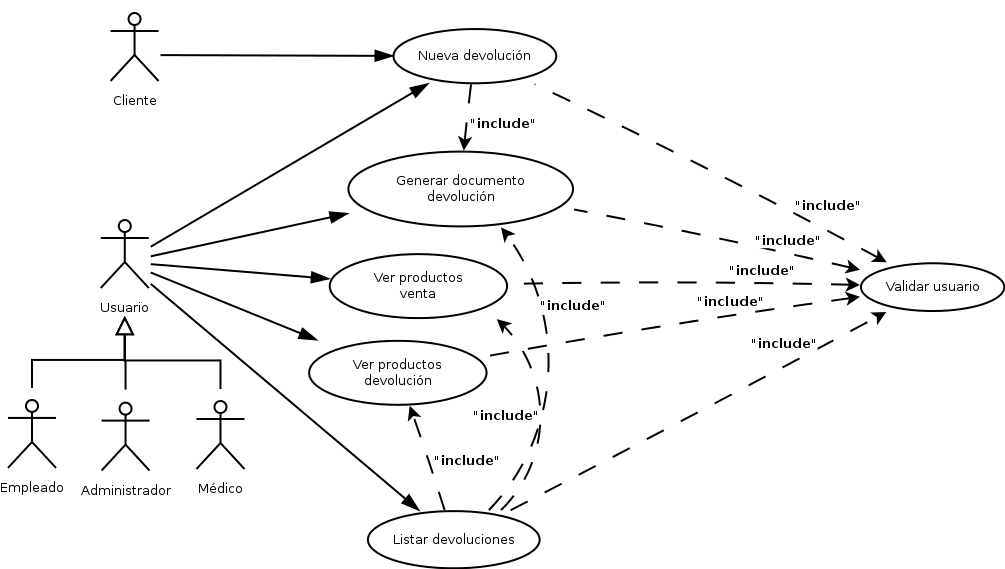
\includegraphics[scale=0.4]{gestiondevoluciones.png}
  \caption{Diagrama caso de uso. Gestión devoluciones}
  \label{cu7}
\end{figure}
\smallskip
\hrule height 1pt
\smallskip
\textbf{Caso de uso: Nueva devolución}
\begin{itemize}\renewcommand{\labelitemi}{$\cdot$}
  \item \textbf{Descripción:} El usuario introduce los datos para registrar una nueva devolución en el sistema.
  \item \textbf{Actores:} Usuario(Principal), Cliente(Secundario)
  \item \textbf{Precondiciones:} Se debe comprobar que el usuario este autenticado en el sistema con el caso de uso Validar usuario.
  \item \textbf{Postcondiciones:} El sistema almacena la devolución en el sistema.
\end{itemize}
\underline{\textbf{Identificación de escenarios:}}
\begin{itemize}\renewcommand{\labelitemi}{$\circ$}
 \item \textbf{Escenario principal:}
         \begin{enumerate}
          \item El caso de uso se inicia cuando el usuario decide crear una nueva devolución.
          \item El sistema muestra por pantalla todas las ventas del sistema para seleccionar.
	\item El usuario selecciona una venta para realizarle la devolución.
          \item El usuario selecciona los productos devueltos de esa venta.
  	  \item El sistema muestra un mensaje de confirmación.
          \item El usuario pulsa SI en el mensaje de confirmación.
 	  \item El sistema almacena el cambio del sistema (auditoria).
          \item La devolución queda almacenada en el sistema y se muestra un mensaje de éxito.
         \end{enumerate}
  \item \textbf{Escenario alternativos:}\\\\
	 4a. El usuario no selecciona ningún producto a devolver.
	      \begin{enumerate}
	       \item El sistema muestra el error y espera que se introduzcan nuevos datos.
	      \end{enumerate}
	 6a. El usuario decide no realizar la devolución.
	      \begin{enumerate}
	       \item El sistema cancela el registro de una nueva devolución en el sistema.
	      \end{enumerate}
         8a. El usuario elige mostrar documento.
	      \begin{enumerate}
	       \item La devolución queda almacenada en el sistema y se muestra el documento por pantalla.
	      \end{enumerate}
          *a. El usuario cancela el proceso de nueva devolución.
\end{itemize}
\smallskip
\hrule height 1pt
\smallskip
\textbf{Caso de uso: Listar devoluciones}
\begin{itemize}\renewcommand{\labelitemi}{$\cdot$}
 \item \textbf{Descripción:} El usuario consulta las devoluciones almacenadas en el sistema.
  \item \textbf{Actores:} Usuario
  \item \textbf{Precondiciones:} Se debe comprobar que el usuario este autenticado en el sistema con el caso de uso Validar usuario.
  \item \textbf{Postcondiciones:} El sistema muestra por pantalla todas las devoluciones almacenadas.
\end{itemize}
\underline{\textbf{Identificación de escenarios:}}
\begin{itemize}\renewcommand{\labelitemi}{$\circ$}
 \item \textbf{Escenario principal:}
         \begin{enumerate}
          \item El caso de uso se inicia cuando el usuario decide consultar las devoluciones.
          \item El sistema muestra la lista de todas las devoluciones del sistema.
          \item El usuario no selecciona un patrón de búsqueda.
          \item El sistema muestra todas las devoluciones.
         \end{enumerate}
  \item \textbf{Escenario alternativos:}\\
  			3a. El usuario introduce un patrón de búsqueda.
  			\begin{enumerate}
  			\item El sistema muestra los datos acordes a ese patrón de búsqueda.
  			\item El usuario puede seleccionar el patrón de búsqueda cuantas veces desee.
  			\end{enumerate}
          *a. El usuario cancela en cualquier momento la consulta de listar devoluciones.
\end{itemize}
\smallskip
\hrule height 1pt
\smallskip
\textbf{Caso de uso: Generar documento devolución}
\begin{itemize}\renewcommand{\labelitemi}{$\cdot$}
 \item \textbf{Descripción:} El usuario decide generar un documento de una devolución.
  \item \textbf{Actores:} Usuario
  \item \textbf{Precondiciones:} La devolución ya existe en el sistema. Se debe comprobar que el usuario este autenticado en el sistema con el caso de uso Validar usuario.
  \item \textbf{Postcondiciones:} El sistema muestra por pantalla el documento devolución generado.
\end{itemize}
\underline{\textbf{Identificación de escenarios:}}
\begin{itemize}\renewcommand{\labelitemi}{$\circ$}
 \item \textbf{Escenario principal:}
         \begin{enumerate}
          \item El caso de uso se inicia cuando el usuario decide generar un documento de devolución.
	  \item El sistema muestra por pantalla el documento de devolución.
         \end{enumerate}
\end{itemize}

\smallskip
\hrule height 1pt
\smallskip
\textbf{Caso de uso: Ver productos devolución}
\begin{itemize}\renewcommand{\labelitemi}{$\cdot$}
 \item \textbf{Descripción:} El usuario decide ver productos devueltos de una venta.
  \item \textbf{Actores:} Usuario
  \item \textbf{Precondiciones:} La venta ya existe en el sistema. Se debe comprobar que el usuario este autenticado en el sistema con el caso de uso Validar usuario.
  \item \textbf{Postcondiciones:} El sistema muestra por pantalla los productos devueltos de una venta.
\end{itemize}
\underline{\textbf{Identificación de escenarios:}}
\begin{itemize}\renewcommand{\labelitemi}{$\circ$}
 \item \textbf{Escenario principal:}
         \begin{enumerate}
          \item El caso de uso se inicia cuando el usuario decide ver los productos devueltos de una venta.
          \item El usuario indica la fecha de la devolución.
	  \item El sistema muestra por pantalla los productos devueltos de la venta en esa fecha.
         \end{enumerate}
\end{itemize}

\subsection{Requisito funcional: Gestión reservas}

\begin{itemize}
 \item El usuario podrá crear una nueva reserva en el sistema.
 \item El usuario podrá consultar e imprimir el listado de todas las reservas del sistema.
 \item El usuario podrá ver los productos asociados a una reserva.
 \item El usuario podrá realizar filtrados de las reservas del sistema.
 \item El usuario podrá generar documentos de reservas.
\item El usuario podrá avisar al cliente cuando el producto vuelva a estar disponible.
\item El usuario podrá convertir a venta una reserva.

\end{itemize}
\begin{figure}[H]
  \centering
    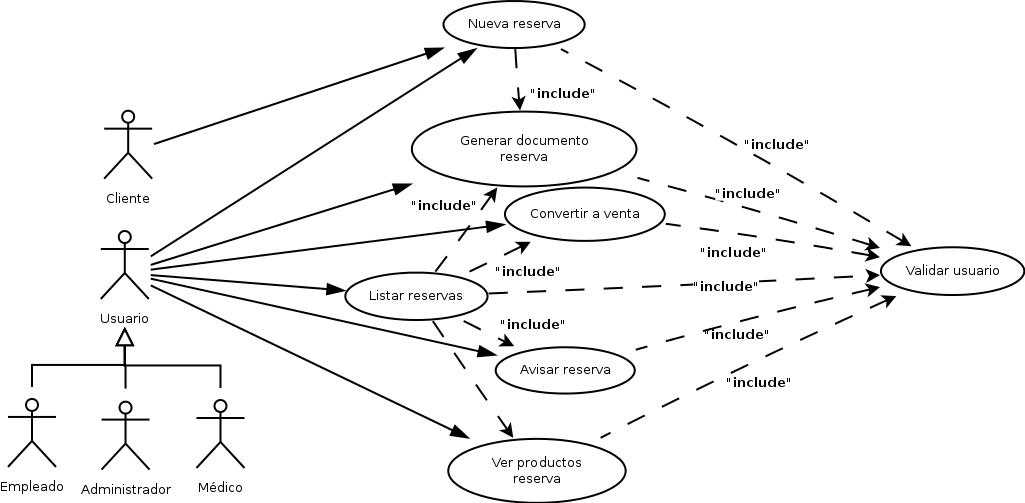
\includegraphics[scale=0.4]{gestionreservas.png}
  \caption{Diagrama caso de uso. Gestión reservas}
  \label{cu7}
\end{figure}
\smallskip
\hrule height 1pt
\smallskip
\textbf{Caso de uso: Nueva reserva}
\begin{itemize}\renewcommand{\labelitemi}{$\cdot$}
  \item \textbf{Descripción:} El usuario introduce los datos para registrar una nueva reserva en el sistema.
  \item \textbf{Actores:} Usuario(Principal), Cliente(Secundario)
  \item \textbf{Precondiciones:} Se debe comprobar que el usuario este autenticado en el sistema con el caso de uso Validar usuario.
  \item \textbf{Postcondiciones:} El usuario almacena la reserva en el sistema.
\end{itemize}
\underline{\textbf{Identificación de escenarios:}}
\begin{itemize}\renewcommand{\labelitemi}{$\circ$}
 \item \textbf{Escenario principal:}
         \begin{enumerate}
          \item El caso de uso se inicia cuando el usuario decide crear una nueva reserva.
	\item El sistema muestra por pantalla todos los clientes para que se puedan seleccionar.
	\item El usuario selecciona el cliente para realizar la reserva.
	\item El sistema muestra por pantalla todos los productos para que se puedan seleccionar.
          \item El usuario introduce los productos y cantidades para la nueva reserva.
	  \item El sistema comprueba que los datos introducidos son correctos.
	 \item El usuario introduce el adelanto del cliente.
	  \item El usuario introduce la forma de pago tarjeta.
  	  \item El sistema muestra un mensaje de confirmación.
          \item El usuario pulsa SI en el mensaje de confirmación.
 	  \item El sistema almacena el cambio del sistema (auditoria).
          \item La reserva queda almacenada en el sistema y se muestra un mensaje de éxito.
         \end{enumerate}
  \item \textbf{Escenario alternativos:}\\\\
	  6a. El usuario introduce de manera incorrecta los datos.
		\begin{enumerate}
		 \item El sistema muestra el error y pide que se introduzcan nuevos datos.
		\end{enumerate}
	7a. El usuario introduce de manera incorrecta el adelanto.
		\begin{enumerate}
		 \item El sistema muestra el error y pide que se introduzca de nuevo el adelanto.
		\end{enumerate}
	8a. El usuario elige el pago con efectivo.
		\begin{enumerate}
		\item El usuario introduce el dinero entregado por el cliente.
		 \item El sistema mostrará en el mensaje de confirmación el cambio a devolver al cliente y la reserva se almacenará con forma de pago efectivo.
		\end{enumerate}
	 10a. El usuario decide no realizar la reserva.
	      \begin{enumerate}
	       \item El sistema cancela el registro de una nueva reserva en el sistema.
	      \end{enumerate}
         12a. El usuario elige mostrar documento reserva.
	      \begin{enumerate}
	       \item La reserva queda almacenada en el sistema y se muestra el documento reserva por pantalla.
	      \end{enumerate}
          *a. El usuario cancela el proceso de nueva reserva.
\end{itemize}
\smallskip
\hrule height 1pt
\smallskip
\textbf{Caso de uso: Listar reservas}
\begin{itemize}\renewcommand{\labelitemi}{$\cdot$}
 \item \textbf{Descripción:} El usuario consulta las reservas almacenadas en el sistema.
  \item \textbf{Actores:} Usuario
  \item \textbf{Precondiciones:} Se debe comprobar que el usuario este autenticado en el sistema con el caso de uso Validar usuario.
  \item \textbf{Postcondiciones:} El sistema muestra por pantalla todas las reservas almacenadas.
\end{itemize}
\underline{\textbf{Identificación de escenarios:}}
\begin{itemize}\renewcommand{\labelitemi}{$\circ$}
 \item \textbf{Escenario principal:}
         \begin{enumerate}
          \item El caso de uso se inicia cuando el usuario decide consultar las reservas.
          \item El sistema muestra la lista de todas las reservas del sistema.
          \item El usuario no selecciona un patrón de búsqueda.
          \item El sistema muestra todas las reservas.
         \end{enumerate}
  \item \textbf{Escenario alternativos:}\\
  			3a. El usuario introduce un patrón de búsqueda.
  			\begin{enumerate}
  			\item El sistema muestra los datos acordes a ese patrón de búsqueda.
  			\item El usuario puede seleccionar el patrón de búsqueda cuantas veces desee.
  			\end{enumerate}
         *a. El usuario cancela en cualquier momento la consulta de listar reservas.
\end{itemize}
\smallskip
\hrule height 1pt
\smallskip
\textbf{Caso de uso: Generar documento reserva}
\begin{itemize}\renewcommand{\labelitemi}{$\cdot$}
 \item \textbf{Descripción:} El usuario decide generar un documento de una reserva.
  \item \textbf{Actores:} Usuario
  \item \textbf{Precondiciones:} La reserva ya existe en el sistema. Se debe comprobar que el usuario este autenticado en el sistema con el caso de uso Validar usuario.
  \item \textbf{Postcondiciones:} El sistema muestra por pantalla el documento reserva generado.
\end{itemize}
\underline{\textbf{Identificación de escenarios:}}
\begin{itemize}\renewcommand{\labelitemi}{$\circ$}
 \item \textbf{Escenario principal:}
         \begin{enumerate}
          \item El caso de uso se inicia cuando el usuario decide generar un documento de reserva.
	  \item El sistema muestra por pantalla el documento de reserva.
         \end{enumerate}
\end{itemize}

\smallskip
\hrule height 1pt
\smallskip
\textbf{Caso de uso: Convertir a venta}
\begin{itemize}\renewcommand{\labelitemi}{$\cdot$}
 \item \textbf{Descripción:} El usuario decide convertir a venta una reserva.
  \item \textbf{Actores:} Usuario
  \item \textbf{Precondiciones:} La reserva ya existe en el sistema. Se debe comprobar que el usuario este autenticado en el sistema con el caso de uso Validar usuario.
  \item \textbf{Postcondiciones:} El sistema almacena una nueva venta asociada con la reserva.
\end{itemize}
\underline{\textbf{Identificación de escenarios:}}
\begin{itemize}\renewcommand{\labelitemi}{$\circ$}
 \item \textbf{Escenario principal:}
         \begin{enumerate}
          \item El caso de uso se inicia cuando el usuario decide convertir una reserva en venta.
	  \item El sistema muestra un mensaje de lo que queda por pagar.
	  \item El usuario introduce la forma de pago tarjeta.
	  \item El sistema muestra un mensaje de confirmación.
	  \item El usuario pulsa en SI en el mensaje.
	  \item EL sistema actualiza la cantidad de los productos reservados.
	  \item El sistema almacena el cambio del sistema (auditoria).
	  \item El sistema almacena la venta asociada a esa reserva y muestra un mensaje por pantalla
         \end{enumerate}
\item \textbf{Escenario alternativos:}\\\\
	3a. El usuario elige el pago con efectivo.
		\begin{enumerate}
		\item El usuario introduce el dinero entregado por el cliente.
		 \item El sistema mostrará en el mensaje de confirmación el cambio a devolver al cliente y la venta se almacenará con forma de pago efectivo.
		\end{enumerate}
	 5a. El usuario decide no realizar la operación.
	      \begin{enumerate}
	       \item El sistema cancela el registro de una nueva venta de la reserva.
	      \end{enumerate}
         6a. El usuario elige mostrar documento venta.
	      \begin{enumerate}
	       \item La venta queda almacenada en el sistema y se muestra el documento venta por pantalla.
	      \end{enumerate}
          *a. El usuario cancela el proceso de nueva venta asociada a la reserva.
\end{itemize}

\smallskip
\hrule height 1pt
\smallskip
\smallskip
\textbf{Caso de uso: Avisar reserva}
\begin{itemize}\renewcommand{\labelitemi}{$\cdot$}
 \item \textbf{Descripción:} El usuario decide avisar al cliente de una reserva.
  \item \textbf{Actores:} Usuario
  \item \textbf{Precondiciones:} La reserva ya existe en el sistema. Se debe comprobar que el usuario este autenticado en el sistema con el caso de uso Validar usuario.
  \item \textbf{Postcondiciones:} El sistema almacena el aviso al cliente.
\end{itemize}
\underline{\textbf{Identificación de escenarios:}}
\begin{itemize}\renewcommand{\labelitemi}{$\circ$}
 \item \textbf{Escenario principal:}
         \begin{enumerate}
          \item El caso de uso se inicia cuando el usuario decide avisar al cliente de una reserva.
	  \item El sistema cambia las cantidades de los productos reservados por apartados.
	  \item El sistema almacena el aviso al cliente.
         \end{enumerate}
\end{itemize}

\smallskip
\hrule height 1pt
\smallskip
\textbf{Caso de uso: Ver productos reserva}
\begin{itemize}\renewcommand{\labelitemi}{$\cdot$}
 \item \textbf{Descripción:} El usuario decide ver productos reservados de una venta.
  \item \textbf{Actores:} Usuario
  \item \textbf{Precondiciones:} La reserva ya existe en el sistema. Se debe comprobar que el usuario este autenticado en el sistema con el caso de uso Validar usuario.
  \item \textbf{Postcondiciones:} El sistema muestra por pantalla los productos reservados.
\end{itemize}
\underline{\textbf{Identificación de escenarios:}}
\begin{itemize}\renewcommand{\labelitemi}{$\circ$}
 \item \textbf{Escenario principal:}
         \begin{enumerate}
          \item El caso de uso se inicia cuando el usuario decide ver los productos reservados.
	  \item El sistema muestra por pantalla los productos reservados.
         \end{enumerate}
\end{itemize}

\subsection{Requisito funcional: Gestión apartados}

\begin{itemize}
 \item El usuario podrá crear una nuevo apartado en el sistema.
 \item El usuario podrá consultar e imprimir el listado de todos los apartados del sistema.
 \item El usuario podrá ver los productos asociados a un apartado.
 \item El usuario podrá realizar filtrados de los apartados del sistema.
 \item El usuario podrá generar documentos de apartados.
\item El usuario podrá convertir a venta un apartado.

\end{itemize}
\begin{figure}[H]
  \centering
    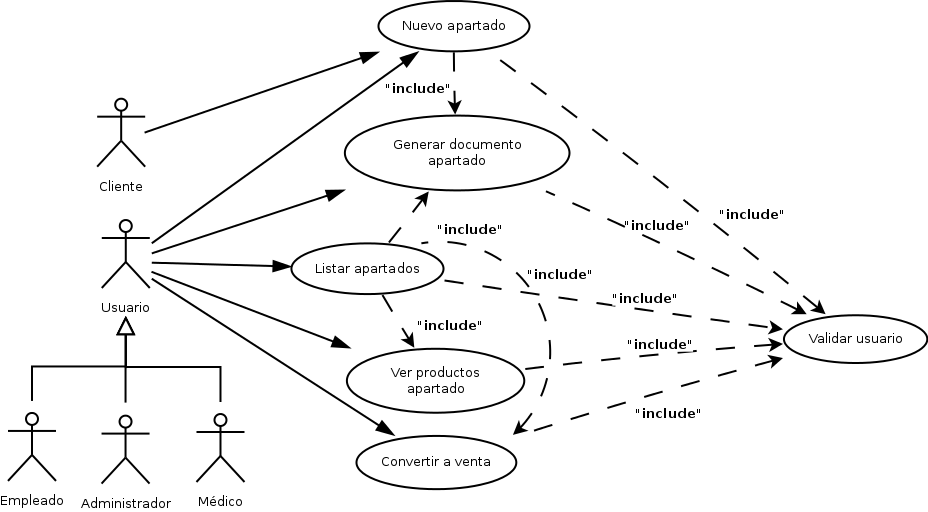
\includegraphics[scale=0.4]{gestionapartados.png}
  \caption{Diagrama caso de uso. Gestión apartados}
  \label{cu7}
\end{figure}
\smallskip
\hrule height 1pt
\smallskip
\textbf{Caso de uso: Nuevo apartado}
\begin{itemize}\renewcommand{\labelitemi}{$\cdot$}
  \item \textbf{Descripción:} El usuario introduce los datos para registrar un nuevo apartado en el sistema.
  \item \textbf{Actores:} Usuario(Principal), Cliente(Secundario)
  \item \textbf{Precondiciones:} Se debe comprobar que el usuario este autenticado en el sistema con el caso de uso Validar usuario.
  \item \textbf{Postcondiciones:} El usuario almacena el apartado en el sistema.
\end{itemize}
\underline{\textbf{Identificación de escenarios:}}
\begin{itemize}\renewcommand{\labelitemi}{$\circ$}
 \item \textbf{Escenario principal:}
         \begin{enumerate}
          \item El caso de uso se inicia cuando el usuario decide crear un nuevo apartado.
	\item El sistema muestra por pantalla todos los clientes para que se puedan seleccionar.
	\item El usuario selecciona al cliente al que quiere realizar el apartado.
	\item El sistema muestra por pantalla todos los productos para que se puedan seleccionar.
          \item El usuario introduce los productos y cantidades para el nuevo apartado.
	  \item El sistema comprueba que los datos introducidos son correctos.
	\item El usuario introduce el adelanto del cliente.
	  \item El usuario introduce la forma de pago tarjeta.
  	  \item El sistema muestra un mensaje de confirmación.
          \item El usuario pulsa SI en el mensaje de confirmación.
 	  \item El sistema almacena el cambio del sistema (auditoria).
          \item El apartado queda almacenado en el sistema y se muestra un mensaje de éxito.
         \end{enumerate}
  \item \textbf{Escenario alternativos:}\\\\
	  6a. El usuario introduce de manera incorrecta los datos.
		\begin{enumerate}
		 \item El sistema muestra el error y pide que se introduzcan nuevos datos.
		\end{enumerate}
	7a. El usuario introduce de manera incorrecta el adelanto.
		\begin{enumerate}
		 \item El sistema muestra el error y pide que se introduzca de nuevo el adelanto.
		\end{enumerate}
	8a. El usuario elige el pago con efectivo.
		\begin{enumerate}
		 \item El usuario introduce el dinero entregado por el cliente.
		 \item El sistema mostrará en el mensaje de confirmación el cambio a devolver al cliente y la venta se almacenará con forma de pago efectivo.
		\end{enumerate}
	 10a. El usuario decide no realizar el apartado.
	      \begin{enumerate}
	       \item El sistema cancela el registro de un nuevo apartado en el sistema.
	      \end{enumerate}
         12a. El usuario elige mostrar documento apartado.
	      \begin{enumerate}
	       \item El apartado queda almacenado en el sistema y se muestra el documento de apartado por pantalla.
	      \end{enumerate}
          *a. El usuario cancela el proceso de nuevo apartado.
\end{itemize}
\smallskip
\hrule height 1pt
\smallskip
\textbf{Caso de uso: Listar apartados}
\begin{itemize}\renewcommand{\labelitemi}{$\cdot$}
 \item \textbf{Descripción:} El usuario consulta los apartados almacenados en el sistema.
  \item \textbf{Actores:} Usuario
  \item \textbf{Precondiciones:} Se debe comprobar que el usuario este autenticado en el sistema con el caso de uso Validar usuario.
  \item \textbf{Postcondiciones:} El sistema muestra por pantalla todos los apartados almacenados.
\end{itemize}
\underline{\textbf{Identificación de escenarios:}}
\begin{itemize}\renewcommand{\labelitemi}{$\circ$}
 \item \textbf{Escenario principal:}
         \begin{enumerate}
          \item El caso de uso se inicia cuando el usuario decide consultar los apartados.
          \item El sistema muestra la lista de todos los apartados del sistema.
          \item El usuario no selecciona un patrón de búsqueda.
          \item El sistema muestra todos los apartados.
         \end{enumerate}
  \item \textbf{Escenario alternativos:}\\
  			3a. El usuario introduce un patrón de búsqueda.
  			\begin{enumerate}
  			\item El sistema muestra los datos acordes a ese patrón de búsqueda.
  			\item El usuario puede seleccionar el patrón de búsqueda cuantas veces desee.
  			\end{enumerate}
         *a. El usuario cancela en cualquier momento la consulta de listar apartados.
\end{itemize}
\smallskip
\hrule height 1pt
\smallskip
\textbf{Caso de uso: Generar documento apartado}
\begin{itemize}\renewcommand{\labelitemi}{$\cdot$}
 \item \textbf{Descripción:} El usuario decide generar un documento de un apartado.
  \item \textbf{Actores:} Usuario
  \item \textbf{Precondicones:} El apartado ya existe en el sistema. Se debe comprobar que el usuario este autenticado en el sistema con el caso de uso Validar usuario.
  \item \textbf{Postcondiciones:} El sistema muestra por pantalla el documento apartado generado.
\end{itemize}
\underline{\textbf{Identificación de escenarios:}}
\begin{itemize}\renewcommand{\labelitemi}{$\circ$}
 \item \textbf{Escenario principal:}
         \begin{enumerate}
          \item El caso de uso se inicia cuando el usuario decide generar un documento de apartado.
	  \item El sistema muestra por pantalla el documento de apartado.
         \end{enumerate}
\end{itemize}

\smallskip
\hrule height 1pt
\smallskip
\textbf{Caso de uso: Convertir a venta}
\begin{itemize}\renewcommand{\labelitemi}{$\cdot$}
 \item \textbf{Descripción:} El usuario decide convertir a venta un apartado.
  \item \textbf{Actores:} Usuario
  \item \textbf{Precondiciones:} El apartado ya existe en el sistema. Se debe comprobar que el usuario este autenticado en el sistema con el caso de uso Validar usuario.
  \item \textbf{Postcondiciones:} El sistema almacena una nueva venta asociada con el apartado.
\end{itemize}
\underline{\textbf{Identificación de escenarios:}}
\begin{itemize}\renewcommand{\labelitemi}{$\circ$}
 \item \textbf{Escenario principal:}
         \begin{enumerate}
          \item El caso de uso se inicia cuando el usuario decide convertir un apartado en venta.
	  \item El sistema muestra un mensaje de lo que queda por pagar.
	  \item El usuario introduce la forma de pago tarjeta.
	  \item El sistema muestra un mensaje de confirmación.
	  \item El usuario pulsa en SI en el mensaje.
	  \item EL sistema actualiza la cantidad de los productos apartados.
	  \item El sistema almacena el cambio del sistema (auditoria).
	  \item El sistema almacena la venta asociada a ese apartado y muestra un mensaje por pantalla
         \end{enumerate}
\item \textbf{Escenario alternativos:}\\\\
	3a. El usuario elige el pago con efectivo.
		\begin{enumerate}
		\item El usuario introduce el dinero entregado por el cliente.
		 \item El sistema mostrará en el mensaje de confirmación el cambio a devolver al cliente y la venta se almacenará con forma de pago efectivo.
		\end{enumerate}
	 5a. El usuario decide no realizar la operación.
	      \begin{enumerate}
	       \item El sistema cancela el registro de una nueva venta del apartado.
	      \end{enumerate}
         6a. El usuario elige mostrar documento venta.
	      \begin{enumerate}
	       \item La venta queda almacenada en el sistema y se muestra el documento venta por pantalla.
	      \end{enumerate}
          *a. El usuario cancela el proceso de nueva venta asociada al apartado.
\end{itemize}

\smallskip
\hrule height 1pt
\smallskip
\textbf{Caso de uso: Ver productos apartado}
\begin{itemize}\renewcommand{\labelitemi}{$\cdot$}
 \item \textbf{Descripción:} El usuario decide ver los productos de un apartado.
  \item \textbf{Actores:} Usuario
  \item \textbf{Precondiciones:} El apartado ya existe en el sistema. Se debe comprobar que el usuario este autenticado en el sistema con el caso de uso Validar usuario.
  \item \textbf{Postcondiciones:} El sistema muestra por pantalla los productos apartados.
\end{itemize}
\underline{\textbf{Identificación de escenarios:}}
\begin{itemize}\renewcommand{\labelitemi}{$\circ$}
 \item \textbf{Escenario principal:}
         \begin{enumerate}
          \item El caso de uso se inicia cuando el usuario decide ver los productos apartados.
	  \item El sistema muestra por pantalla los productos apartados.
         \end{enumerate}
\end{itemize}

\subsection{Requisito funcional: Gestión citas e informes}

\begin{itemize}
 \item El usuario podrá crear una nueva cita en el sistema.
 \item El usuario podrá consultar un informe en el sistema.
 \item El usuario podrá eliminar una cita del sistema.
 \item El usuario podrá consultar e imprimir el listado de todas las citas del sistema.
 \item El usuario podrá realizar filtrados de las citas del sistema.
 \item El usuario podrá consultar e imprimir el listado de todos los informes del sistema.
 \item El usuario podrá realizar filtrados de los informes del sistema. 
 \item El médico podrá crear un nuevo informe sin cita en el sistema.
 \item El médico podrá crear un nuevo informe con cita en el sistema.

\end{itemize}
\begin{figure}[H]
  \centering
    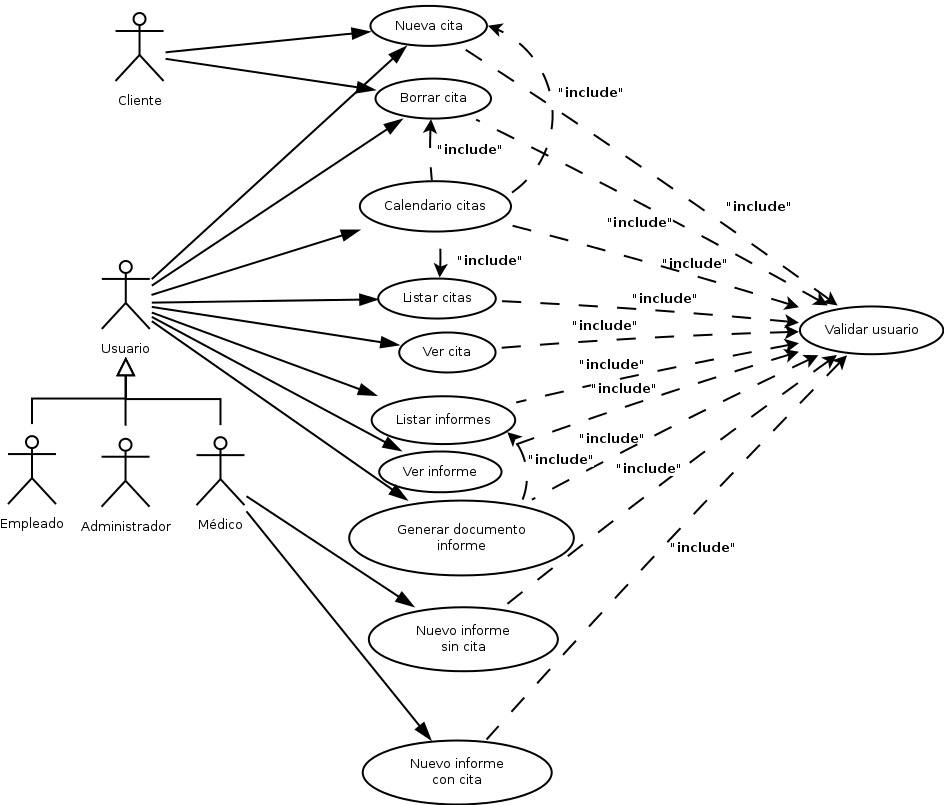
\includegraphics[scale=0.5]{gestioncitaseinformes.png}
  \caption{Diagrama caso de uso. Gestión citas e informes}
  \label{cu8}
\end{figure}
\smallskip
\hrule height 1pt
\smallskip
\textbf{Caso de uso: Nueva cita}
\begin{itemize}\renewcommand{\labelitemi}{$\cdot$}
  \item \textbf{Descripción:} El usuario introduce los datos para registrar una nueva cita en el sistema.
  \item \textbf{Actores:} Usuario(Principal) Cliente(Secundario)
  \item \textbf{Precondiciones:} Se debe comprobar que el usuario este autenticado en el sistema con el caso de uso Validar usuario.
  \item \textbf{Postcondiciones:} El usuario almacena la cita en el sistema.
\end{itemize}
\underline{\textbf{Identificación de escenarios:}}
\begin{itemize}\renewcommand{\labelitemi}{$\circ$}
 \item \textbf{Escenario principal:}
         \begin{enumerate}
          \item El caso de uso se inicia cuando el usuario decide crear una nueva cita.
          \item El usuario selecciona el dia que quiere crear la cita.
	  \item El sistema muestra por pantalla los clientes y los médicos para que el usuario seleccione.
	  \item El usuario introduce el cliente y el médico de la cita.
          \item El sistema comprueba que los datos introducidos son correctos.
 	  \item El sistema almacena el cambio del sistema (auditoria).
          \item La cita queda almacenada en el sistema y se muestra por pantalla.
         \end{enumerate}
  \item \textbf{Escenario alternativos:}\\\\
	5a. La fecha introducida esta ocupada por el médico o el cliente.
		\begin{enumerate}
		 \item El sistema muestra el error y pide que se introduzcan nuevos datos.
		\end{enumerate}
          *a. El usuario cancela en cualquier momento el proceso de nueva cita.
\end{itemize}
\smallskip
\hrule height 1pt
\smallskip
\textbf{Caso de uso: Borrar cita}
\begin{itemize}\renewcommand{\labelitemi}{$\cdot$}
 \item \textbf{Descripción:} El usuario decide borrar una cita del sistema.
  \item \textbf{Actores:} Usuario(Principal), Cliente(Secundario)
  \item \textbf{Precondiciones:} La cita existe en el sistema. Se debe comprobar que el usuario este autenticado en el sistema con el caso de uso Validar usuario.
  \item \textbf{Postcondiciones:} El sistema elimina la cita del sistema.
\end{itemize}
\underline{\textbf{Identificación de escenarios:}}
\begin{itemize}\renewcommand{\labelitemi}{$\circ$}
 \item \textbf{Escenario principal:}
         \begin{enumerate}
          \item El caso de uso se inicia cuando el usuario decide borrar una cita.
          \item El usuario selecciona la cita que quiere eliminar.
          \item El sistema muestra un mensaje de confirmación.
          \item El administrador pulsa SI en el mensaje de confirmación.
 	  \item El sistema almacena el cambio del sistema (auditoria).
          \item El sistema elimina la cita seleccionada.
         \end{enumerate}
  \item \textbf{Escenario alternativos:}\\
  			4a. El usuario cancela en el mensaje de confirmación.
  			\begin{enumerate}
  			\item El sistema cancela el proceso de eliminación de una cita.
  			\end{enumerate}
          *a. El usuario cancela en cualquier momento la eliminación de una cita.
\end{itemize}
\smallskip
\hrule height 1pt
\smallskip

\textbf{Caso de uso: Listar citas}
\begin{itemize}\renewcommand{\labelitemi}{$\cdot$}
 \item \textbf{Descripción:} El usuario decide listar todas las citas del sistema.
  \item \textbf{Actores:} Usuario
  \item \textbf{Precondiciones:} Se debe comprobar que el usuario este autenticado en el sistema con el caso de uso Validar usuario.
  \item \textbf{Postcondiciones:} El sistema muestra un listado de todas las citas del sistema.
\end{itemize}
\underline{\textbf{Identificación de escenarios:}}
\begin{itemize}\renewcommand{\labelitemi}{$\circ$}
 \item \textbf{Escenario principal:}
         \begin{enumerate}
          \item El caso de uso se inicia cuando el usuario decide listar las citas del sistema.
	  \item El sistema muestra por pantalla todas las citas del sistema.
         \end{enumerate}
\end{itemize}

\smallskip
\hrule height 1pt
\smallskip

\textbf{Caso de uso: Calendario citas}
\begin{itemize}\renewcommand{\labelitemi}{$\cdot$}
 \item \textbf{Descripción:} El usuario decide mostrar en el calendario todas las citas del sistema.
  \item \textbf{Actores:} Usuario
  \item \textbf{Precondiciones:} Se debe comprobar que el usuario este autenticado en el sistema con el caso de uso Validar usuario.
  \item \textbf{Postcondiciones:} El sistema muestra un calendario con todas las citas del sistema.
\end{itemize}
\underline{\textbf{Identificación de escenarios:}}
\begin{itemize}\renewcommand{\labelitemi}{$\circ$}
 \item \textbf{Escenario principal:}
         \begin{enumerate}
          \item El caso de uso se inicia cuando el usuario decide consultar el calendario de citas del sistema.
	  \item El sistema muestra por pantalla todas las citas del sistema en el calendario.
         \end{enumerate}
\end{itemize}

\smallskip
\hrule height 1pt
\smallskip
\textbf{Caso de uso: Listar informes}
\begin{itemize}\renewcommand{\labelitemi}{$\cdot$}
 \item \textbf{Descripción:} El usuario decide listar todos los informes del sistema.
  \item \textbf{Actores:} Usuario
  \item \textbf{Precondiciones:} Se debe comprobar que el usuario este autenticado en el sistema con el caso de uso Validar usuario.
  \item \textbf{Postcondiciones:} El sistema muestra un listado de todos los informes del sistema.
\end{itemize}
\underline{\textbf{Identificación de escenarios:}}
\begin{itemize}\renewcommand{\labelitemi}{$\circ$}
 \item \textbf{Escenario principal:}
         \begin{enumerate}
          \item El caso de uso se inicia cuando el usuario decide listar los informes.
	  \item El sistema muestra por pantalla todos los informes del sistema.
         \end{enumerate}
\end{itemize}

\smallskip
\hrule height 1pt
\smallskip
\textbf{Caso de uso: Nuevo informe con cita}
\begin{itemize}\renewcommand{\labelitemi}{$\cdot$}
 \item \textbf{Descripción:} El médico decide crear un informe de una cita.
  \item \textbf{Actores:} Médico
  \item \textbf{Precondiciones:} La cita ya existe en el sistema. Se debe comprobar que el médico este autenticado en el sistema con el caso de uso Validar usuario.
  \item \textbf{Postcondiciones:} El sistema guarda en el sistema y muestra el informe de la cita.
\end{itemize}
\underline{\textbf{Identificación de escenarios:}}
\begin{itemize}\renewcommand{\labelitemi}{$\circ$}
 \item \textbf{Escenario principal:}
         \begin{enumerate}
          \item El caso de uso se inicia cuando el médico decide crear un informe de una cita.
          \item El sistema muestra las citas que le pertenecen.
          \item El médico selecciona la cita a la que generar el informe.
          \item El médico introduce los datos del informe.
	  \item El sistema muestra un mensaje de confirmación.
          \item El médico pulsa SI en el mensaje de confirmación.
 	  \item El sistema almacena el cambio del sistema (auditoria).
	  \item El sistema almacena y muestra por pantalla el nuevo informe.
         \end{enumerate}
\item \textbf{Escenario alternativos:}\\
  			6a. El usuario indica NO en el mensaje de confirmación.
  			\begin{enumerate}
  			\item El sistema cancela el proceso de generar un nuevo informe con cita.
  			\end{enumerate}
          *a. El médico cancela en cualquier momento la generación de un nuevo informe con cita.
\end{itemize}

\smallskip
\hrule height 1pt
\smallskip
\textbf{Caso de uso: Nuevo informe sin cita}
\begin{itemize}\renewcommand{\labelitemi}{$\cdot$}
 \item \textbf{Descripción:} El médico decide crear un informe de un cliente.
  \item \textbf{Actores:} Médico
  \item \textbf{Precondiciones:} Se debe comprobar que el médico este autenticado en el sistema con el caso de uso Validar usuario.
  \item \textbf{Postcondiciones:} El sistema guarda en el sistema una nueva cita y muestra el informe generado asociado.
\end{itemize}
\underline{\textbf{Identificación de escenarios:}}
\begin{itemize}\renewcommand{\labelitemi}{$\circ$}
 \item \textbf{Escenario principal:}
         \begin{enumerate}
          \item El caso de uso se inicia cuando el médico decide crear un informe de un cliente.
	  \item El sistema muestra una lista con todos los clientes del sistema.
          \item El médico selecciona el cliente al cual generar el informe.
          \item El médico introduce los datos del informe.
	  \item El sistema muestra un mensaje de confirmación.
          \item El médico pulsa SI en el mensaje de confirmación.
 	  \item El sistema almacena el cambio del sistema (auditoria).
	  \item El sistema crea una nueva cita. Almacena y muestra por pantalla el nuevo informe.
         \end{enumerate}
\item \textbf{Escenario alternativos:}\\
  			6a. El usuario indica NO en el mensaje de confirmación.
  			\begin{enumerate}
  			\item El sistema cancela el proceso de generar un nuevo informe sin cita.
  			\end{enumerate}
          *a. El médico cancela en cualquier momento la generación de un informe a un cliente.
\end{itemize}


\smallskip
\hrule height 1pt
\smallskip
\textbf{Caso de uso: Ver cita}
\begin{itemize}\renewcommand{\labelitemi}{$\cdot$}
 \item \textbf{Descripción:} El usuario decide consultar una cita del sistema.
  \item \textbf{Actores:} Usuario
  \item \textbf{Precondiciones:} Se debe comprobar que el usuario este autenticado en el sistema con el caso de uso Validar usuario.
  \item \textbf{Postcondiciones:} El sistema muestra por pantalla la información de la cita del cliente.
\end{itemize}
\underline{\textbf{Identificación de escenarios:}}
\begin{itemize}\renewcommand{\labelitemi}{$\circ$}
 \item \textbf{Escenario principal:}
         \begin{enumerate}
          \item El caso de uso se inicia cuando el usuario decide consultar una cita.
	  \item El sistema muestra la cita del cliente por pantalla.
         \end{enumerate}
\end{itemize}

\smallskip
\hrule height 1pt
\smallskip
\textbf{Caso de uso: Ver informe}
\begin{itemize}\renewcommand{\labelitemi}{$\cdot$}
 \item \textbf{Descripción:} El usuario decide consultar un informe de un cliente del sistema.
  \item \textbf{Actores:} Usuario
  \item \textbf{Precondiciones:} Se debe comprobar que el usuario este autenticado en el sistema con el caso de uso Validar usuario.
  \item \textbf{Postcondiciones:} El sistema muestra por pantalla el informe del cliente.
\end{itemize}
\underline{\textbf{Identificación de escenarios:}}
\begin{itemize}\renewcommand{\labelitemi}{$\circ$}
 \item \textbf{Escenario principal:}
         \begin{enumerate}
          \item El caso de uso se inicia cuando el usuario decide consultar un informe.
	  \item El sistema muestra por pantalla el informe del cliente.
         \end{enumerate}
\end{itemize}

\smallskip
\hrule height 1pt
\smallskip
\textbf{Caso de uso: Generar documento informe}
\begin{itemize}\renewcommand{\labelitemi}{$\cdot$}
 \item \textbf{Descripción:} El usuario decide generar un documento de un informe.
  \item \textbf{Actores:} Usuario
  \item \textbf{Precondicones:} El informe ya existe en el sistema. Se debe comprobar que el usuario este autenticado en el sistema con el caso de uso Validar usuario.
  \item \textbf{Postcondiciones:} El sistema muestra por pantalla el documento informe generado.
\end{itemize}
\underline{\textbf{Identificación de escenarios:}}
\begin{itemize}\renewcommand{\labelitemi}{$\circ$}
 \item \textbf{Escenario principal:}
         \begin{enumerate}
          \item El caso de uso se inicia cuando el usuario decide generar un documento de un cierto informe.
	  \item El sistema muestra por pantalla el documento del informe.
         \end{enumerate}
\end{itemize}

\subsection{Requisito funcional: Gestión festivos}

\begin{itemize}
 \item El administrador podrá crear un nuevo festivo en el sistema.
 \item El administrador podrá eliminar un festivo del sistema.
 \item El administrador podrá consultar e imprimir el listado de todas los festivos del sistema.
 \item El administrador podrá realizar filtrados de los festivos del sistema.

\end{itemize}
\begin{figure}[H]
  \centering
    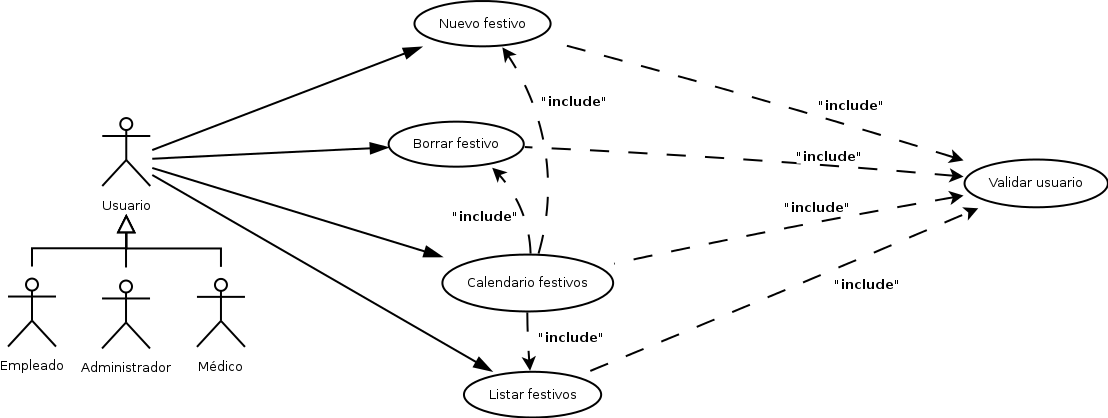
\includegraphics[scale=0.4]{gestionfestivos.png}
  \caption{Diagrama caso de uso. Gestión festivos}
  \label{cu8}
\end{figure}
\smallskip
\hrule height 1pt
\smallskip
\textbf{Caso de uso: Nuevo festivo}
\begin{itemize}\renewcommand{\labelitemi}{$\cdot$}
  \item \textbf{Descripción:} El administrador introduce los datos para registrar un nuevo festivo en el sistema.
  \item \textbf{Actores:} Administrador
  \item \textbf{Precondiciones:} Se debe comprobar que el administrador este autenticado en el sistema con el caso de uso Validar usuario.
  \item \textbf{Postcondiciones:} El usuario almacena el festivo en el sistema.
\end{itemize}
\underline{\textbf{Identificación de escenarios:}}
\begin{itemize}\renewcommand{\labelitemi}{$\circ$}
 \item \textbf{Escenario principal:}
         \begin{enumerate}
          \item El caso de uso se inicia cuando el administrador decide crear un nuevo festivo.
	  \item El sistema muestra el calendario.
          \item El usuario selecciona el día que quiere crear el festivo.
          \item El sistema comprueba que los datos introducidos son correctos.
	  \item El sistema muestra un mensaje de confirmación.
          \item El médico pulsa SI en el mensaje de confirmación.
 	  \item El sistema almacena el cambio del sistema (auditoria).
          \item El festivo queda almacenado en el sistema y se muestra por pantalla.
         \end{enumerate}
  \item \textbf{Escenario alternativos:}\\\\
	4a. El empleado elige una fecha en la cual ya existen citas.
  			\begin{enumerate}
  			\item El sistema cancela el registro de nuevo festivo y muestra el error.
  			\end{enumerate}
	6a. El usuario indica NO en el mensaje de confirmación.
  			\begin{enumerate}
  			\item El sistema cancela el proceso de generar un nuevo informe sin cita.
  			\end{enumerate}
          *a. El usuario cancela en cualquier momento el proceso de un nuevo festivo.
\end{itemize}
\smallskip
\hrule height 1pt
\smallskip
\textbf{Caso de uso: Borrar festivo}
\begin{itemize}\renewcommand{\labelitemi}{$\cdot$}
 \item \textbf{Descripción:} El administrador decide borrar un festivo del sistema.
  \item \textbf{Actores:} Administrador
  \item \textbf{Precondiciones:} El festivo ya existe en el sistema. Se debe comprobar que el administrador este autenticado en el sistema con el caso de uso Validar usuario.
  \item \textbf{Postcondiciones:} El sistema elimina el festivo del sistema.
\end{itemize}
\underline{\textbf{Identificación de escenarios:}}
\begin{itemize}\renewcommand{\labelitemi}{$\circ$}
 \item \textbf{Escenario principal:}
         \begin{enumerate}
          \item El caso de uso se inicia cuando el usuario decide borrar un festivo.
          \item El administrador selecciona el festivo que quiere eliminar.
          \item El sistema muestra un mensaje de confirmación.
          \item El administrador pulsa SI en el mensaje de confirmación.
 	  \item El sistema almacena el cambio del sistema (auditoria).
          \item El sistema elimina el festivo seleccionado.
         \end{enumerate}
  \item \textbf{Escenario alternativos:}\\
  			4a. El usuario cancela en el mensaje de confirmación.
  			\begin{enumerate}
  			\item El sistema cancela el proceso de eliminación de un festivo.
  			\end{enumerate}
          *a. El usuario cancela en cualquier momento la eliminación de un festivo.
\end{itemize}

\smallskip
\hrule height 1pt
\smallskip

\textbf{Caso de uso: Listar festivos}
\begin{itemize}\renewcommand{\labelitemi}{$\cdot$}
 \item \textbf{Descripción:} El administrador decide listar todos los festivos del sistema.
  \item \textbf{Actores:} Administrador
  \item \textbf{Precondiciones:} Se debe comprobar que el administrador este autenticado en el sistema con el caso de uso Validar usuario.
  \item \textbf{Postcondiciones:} El sistema muestra un listado de todos los festivos del sistema.
\end{itemize}
\underline{\textbf{Identificación de escenarios:}}
\begin{itemize}\renewcommand{\labelitemi}{$\circ$}
 \item \textbf{Escenario principal:}
         \begin{enumerate}
          \item El caso de uso se inicia cuando el usuario decide listar todos los festivos del sistema.
	  \item El sistema muestra por pantalla todos los festivos.
         \end{enumerate}
\end{itemize}

\smallskip
\hrule height 1pt
\smallskip
\textbf{Caso de uso: Calendario festivos}
\begin{itemize}\renewcommand{\labelitemi}{$\cdot$}
 \item \textbf{Descripción:} El usuario decide mostrar el calendario de festivos.
  \item \textbf{Actores:} Administrador
  \item \textbf{Precondiciones:} Se debe comprobar que el administrador este autenticado en el sistema con el caso de uso Validar usuario.
  \item \textbf{Postcondiciones:} El sistema muestra el calendario con todos los festivos almacenados en el sistema.
\end{itemize}
\underline{\textbf{Identificación de escenarios:}}
\begin{itemize}\renewcommand{\labelitemi}{$\circ$}
 \item \textbf{Escenario principal:}
         \begin{enumerate}
          \item El caso de uso se inicia cuando el usuario decide mostrar el calendario de festivos.
	  \item El sistema muestra por pantalla todos los festivos en el calendario.
         \end{enumerate}
\end{itemize}

\subsection{Requisito funcional: Gestión de entradas y salidas del sistema}

\begin{itemize}
 \item El usuario podrá entrar al sistema mediante un formulario de logueo.
 \item El usuario tendrá la posibilidad de recuperar la contraseña por si está ha sido olvidada.
 \item El usuario deberá salir del sistema mediante el botón "Salir".

\end{itemize}
\begin{figure}[H]
  \centering
    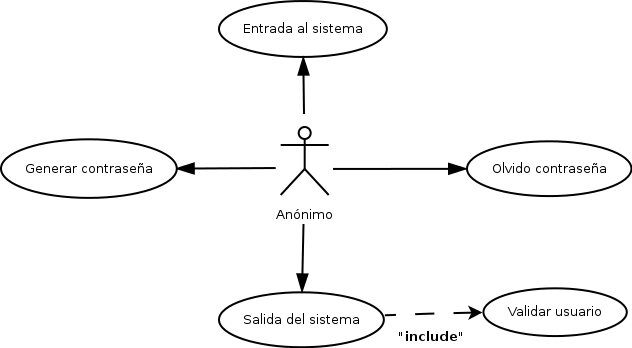
\includegraphics[scale=0.5]{login.png}
  \caption{Diagrama caso de uso. Gestión de entradas y salidas}
  \label{cu8}
\end{figure}
\smallskip
\hrule height 1pt
\smallskip
\textbf{Caso de uso: Entrada al sistema}
\begin{itemize}\renewcommand{\labelitemi}{$\cdot$}
  \item \textbf{Descripción:} El usuario introduce los datos para ingresar al sistema.
  \item \textbf{Actores:} Usuario
  \item \textbf{Postcondiciones:} El usuario ingresa en el sistema.
\end{itemize}
\underline{\textbf{Identificación de escenarios:}}
\begin{itemize}\renewcommand{\labelitemi}{$\circ$}
 \item \textbf{Escenario principal:}
         \begin{enumerate}
          \item El caso de uso se inicia cuando el usuario decide entrar en el sistema.
          \item El usuario introduce nombre de usuario y contraseña.
          \item El sistema comprueba que los datos introducidos son correctos.
	  \item El sistema almacena la entrada del usuario.
          \item El usuario entra en el sistema y se muestra la pantalla principal.
         \end{enumerate}
  \item \textbf{Escenario alternativos:}\\\\
		2a. El usuario no introduce la contraseña correcta.
  			\begin{enumerate}
  			\item El sistema muestra el error y pide nuevos datos.
  			\end{enumerate}
		2b. El usuario no introduce datos.
  			\begin{enumerate}
  			\item El sistema muestra el error y pide nuevos datos.
  			\end{enumerate}
          *a. El usuario cancela en cualquier momento la inserción al sistema.
\end{itemize}

\smallskip
\hrule height 1pt
\smallskip
\textbf{Caso de uso: Salida del sistema}
\begin{itemize}\renewcommand{\labelitemi}{$\cdot$}
 \item \textbf{Descripción:} El usuario decide salir del sistema.
  \item \textbf{Actores:} Usuario
  \item \textbf{Precondiciones:} Se debe comprobar que el usuario este autenticado en el sistema con el caso de uso Validar usuario.
  \item \textbf{Postcondiciones:} El sistema realiza la salida del usuario del sistema.
\end{itemize}
\underline{\textbf{Identificación de escenarios:}}
\begin{itemize}\renewcommand{\labelitemi}{$\circ$}
 \item \textbf{Escenario principal:}
         \begin{enumerate}
          \item El caso de uso se inicia cuando el usuario decide salir del sistema.
	 \item El sistema almacena la salida del sistema.
          \item El sistema facilita la salida del usuario del sistema.
	  \item El sistema muestra la pantalla principal de entrada al sistema.
         \end{enumerate}
\end{itemize}
\smallskip
\hrule height 1pt
\smallskip
\textbf{Caso de uso: Olvido de contraseña}
\begin{itemize}\renewcommand{\labelitemi}{$\cdot$}
 \item \textbf{Descripción:} El usuario decide recuperar su contraseña.
  \item \textbf{Actores:} Usuario.
  \item \textbf{Postcondiciones:} El sistema manda un email con un link para poder generar una nueva contraseña para el usuario.
\end{itemize}
\underline{\textbf{Identificación de escenarios:}}
\begin{itemize}\renewcommand{\labelitemi}{$\circ$}
 \item \textbf{Escenario principal:}
         \begin{enumerate}
          \item El caso de uso se inicia cuando el usuario decide recuperar su contraseña.
          \item El usuario introduce su email.
          \item El sistema comprueba que ese email pertenece a un cliente.
          \item El sistema manda un email con un link de generación de contraseña.
         \end{enumerate}
  \item \textbf{Escenario alternativos:}\\
  			3a. El email no pertenece a ningún usuario.
  			\begin{enumerate}
  			\item El sistema muestra el error y pide nuevo email.
  			\end{enumerate}
          *a. El usuario cancela en cualquier momento la recuperación de la contraseña.
\end{itemize}

\smallskip
\hrule height 1pt
\smallskip
\textbf{Caso de uso: Generar Contraseña}
\begin{itemize}\renewcommand{\labelitemi}{$\cdot$}
 \item \textbf{Descripción:} El usuario pulsa el link de generación de nueva contraseña.
  \item \textbf{Actores:} Usuario.
  \item \textbf{Postcondiciones:} El sistema almacena una nueva contraseña aleatoria para el usuario.
\end{itemize}
\underline{\textbf{Identificación de escenarios:}}
\begin{itemize}\renewcommand{\labelitemi}{$\circ$}
 \item \textbf{Escenario principal:}
         \begin{enumerate}
          \item El caso de uso se inicia cuando el usuario pulsa en el link de recuperación.
          \item El sistema comprueba que ese link es válido.
          \item El sistema genera una nueva contraseña y la manda por email al usuario.
         \end{enumerate}
  \item \textbf{Escenario alternativos:}\\
  			3a. El link no es válido.
  			\begin{enumerate}
  			\item El sistema muestra el error.
  			\end{enumerate}
\end{itemize}

\subsection{Requisito funcional: Estadísticas}

\begin{itemize}
 \item El usuario podrá ver sus propias estadísticas.
 \item El administrador podrá ver las estadísticas de la empresa.
 \item Se podrán exportar las estadísticas a distintos formatos.

\end{itemize}
\begin{figure}[H]
  \centering
    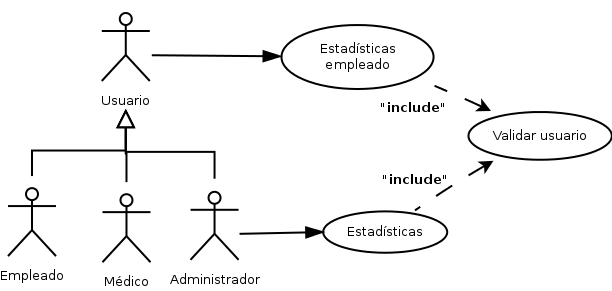
\includegraphics[scale=0.5]{estadisticas.png}
  \caption{Diagrama caso de uso. Estadisticas}
  \label{cu8}
\end{figure}
\smallskip
\hrule height 1pt
\smallskip
\textbf{Caso de uso: Estadisticas empleado}
\begin{itemize}\renewcommand{\labelitemi}{$\cdot$}
  \item \textbf{Descripción:} El usuario decide observar sus estadísticas.
  \item \textbf{Actores:} Usuario
  \item \textbf{Precondiciones:} Se debe comprobar que el usuario este autenticado en el sistema con el caso de uso Validar usuario.
  \item \textbf{Postcondiciones:} El sistema muestra por pantalla las distintas estadísticas del empleado.
\end{itemize}
\underline{\textbf{Identificación de escenarios:}}
\begin{itemize}\renewcommand{\labelitemi}{$\circ$}
 \item \textbf{Escenario principal:}
         \begin{enumerate}
          \item El caso de uso se inicia cuando el usuario decide consultar sus estadísticas.
          \item El sistema muestra por pantalla las estadísticas.
         \end{enumerate}
  \item \textbf{Escenario alternativos:}\\\\
          *a. El usuario cancela en cualquier momento la consulta de sus estadísticas.
\end{itemize}

\smallskip
\hrule height 1pt
\smallskip
\textbf{Caso de uso: Estadisticas}
\begin{itemize}\renewcommand{\labelitemi}{$\cdot$}
  \item \textbf{Descripción:} El administrador decide observar las estadísticas del sistema.
  \item \textbf{Actores:} Administrador
  \item \textbf{Precondiciones:} Se debe comprobar que el administrador este autenticado en el sistema con el caso de uso Validar usuario.
  \item \textbf{Postcondiciones:} El sistema muestra por pantalla las distintas estadísticas generadas.
\end{itemize}
\underline{\textbf{Identificación de escenarios:}}
\begin{itemize}\renewcommand{\labelitemi}{$\circ$}
 \item \textbf{Escenario principal:}
         \begin{enumerate}
          \item El caso de uso se inicia cuando el empleado decide consultar las estadísticas.
          \item El sistema muestra por pantalla las estadísticas del sistema.
         \end{enumerate}
  \item \textbf{Escenario alternativos:}\\\\
          *a. El administrador cancela en cualquier momento la consulta de las estadísticas del sistema.
\end{itemize}

\subsection{Requisito funcional: Gestión de pedidos}

\begin{itemize}
 \item El usuario podrá registrar un nuevo pedido a un proveedor.
 \item El usuario podrá consultar e imprimir el listado de todos los pedidos del sistema.
 \item El usuario podrá recepcionar la llegada de los pedidos.
 \item El usuario podrá ver los productos asociados al pedido.
 \item El usuario podrá realizar filtrados de los pedidos del sistema.
 \item El usuario podrá generar un documento de pedido.
\end{itemize}
\begin{figure}[H]
  \centering
    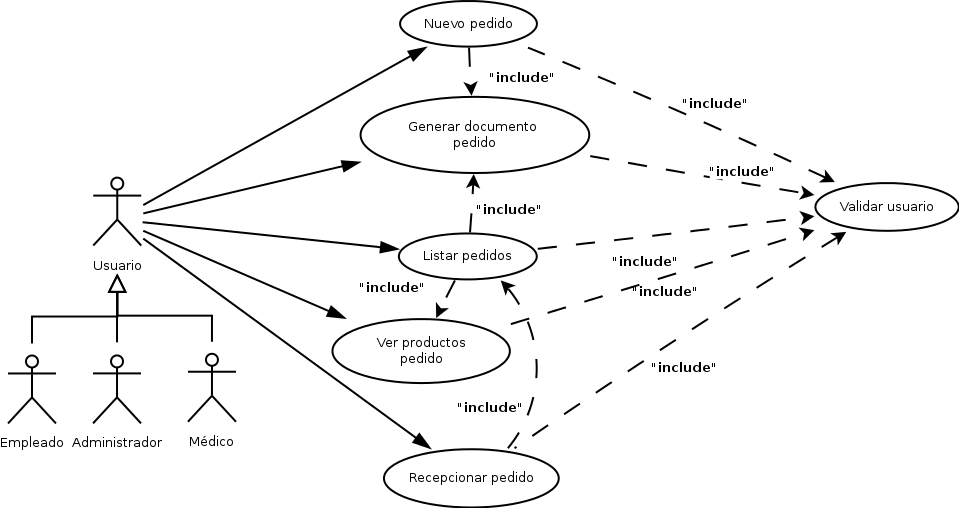
\includegraphics[scale=0.4]{gestionpedidos.png}
  \caption{Diagrama caso de uso. Gestión de pedidos}
  \label{cu1}
\end{figure}
\smallskip
\hrule height 1pt
\smallskip
\textbf{Caso de uso: Registrar pedido}
\begin{itemize}\renewcommand{\labelitemi}{$\cdot$}
 \item \textbf{Descripción:} El usuario introduce los datos para registrar un nuevo pedido en el sistema.
  \item \textbf{Actores:} Usuario
  \item \textbf{Precondiciones:} Se debe comprobar que el usuario este autenticado en el sistema con el caso de uso Validar usuario.
  \item \textbf{Postcondiciones:} El sistema almacena al pedido en el sistema.
\end{itemize}
\underline{\textbf{Identificación de escenarios:}}
\begin{itemize}\renewcommand{\labelitemi}{$\circ$}
 \item \textbf{Escenario principal:}
         \begin{enumerate}
          \item El caso de uso se inicia cuando el usuario decide registrar un nuevo pedido.
          \item El sistema muestra una lista de los proveedores para realizar el pedido.
          \item El usuario selecciona el proveedor para realizar el pedido.
         \item  El sistema muestra por pantalla los productos que suministra el proveedor.
          \item El usuario indica las cantidades y productos que desea añadir al pedido.
          \item El sistema comprueba que los datos introducidos son correctos. 
          \item El sistema muestra un mensaje de confirmación.
          \item El administrador pulsa SI en el mensaje de confirmación.
 	  \item El sistema almacena el cambio del sistema (auditoria).
          \item El pedido queda registrado en el sistema y el sistema muestra un mensaje de éxito.
         \end{enumerate}
  \item \textbf{Escenario alternativos:}\\\\
	6a. El usuario introduce de manera incorrecta los datos.
		\begin{enumerate}
		 \item El sistema muestra el error y pide que se introduzcan nuevos datos.
		\end{enumerate}
   	8a. El administrador decide no registrar un nuevo pedido
	      \begin{enumerate}
	       \item El sistema cancela el registro de un nuevo pedido y pide nuevos datos.
	      \end{enumerate}
          *a. El usuario cancela en cualquier momento el proceso de registro de un nuevo pedido.
\end{itemize}
\smallskip
\hrule height 1pt
\smallskip
\textbf{Caso de uso: Recepcionar pedido}
\begin{itemize}\renewcommand{\labelitemi}{$\cdot$}
 \item \textbf{Descripción:} El usuario recepciona un pedido en el sistema.
  \item \textbf{Actores:} Usuario
  \item \textbf{Precondiciones:} El pedido ya existe en el sistema. Se debe comprobar que el usuario este autenticado en el sistema con el caso de uso Validar usuario.
  \item \textbf{Postcondiciones:} El sistema recepciona el pedido en el sistema.
\end{itemize}
\underline{\textbf{Identificación de escenarios:}}
\begin{itemize}\renewcommand{\labelitemi}{$\circ$}
 \item \textbf{Escenario principal:}
         \begin{enumerate}
          \item El caso de uso se inicia cuando el usuario decide recepcionar un nuevo pedido.
          \item El sistema actualiza los stocks de los productos que han llegado en el pedido.
 	  \item El sistema almacena el cambio del sistema (auditoria).
          \item El sistema guarda los cambios.
       \end{enumerate}
\end{itemize}

\smallskip
\hrule height 1pt
\smallskip
\textbf{Caso de uso: Listar pedidos}
\begin{itemize}\renewcommand{\labelitemi}{$\cdot$}
 \item \textbf{Descripción:} El usuario decide consultar los pedidos en el sistema.
  \item \textbf{Actores:} Usuario
  \item \textbf{Precondiciones:} Se debe comprobar que el usuario este autenticado en el sistema con el caso de uso Validar usuario.
  \item \textbf{Postcondiciones:} El sistema muestra por pantalla todos los pedidos.
\end{itemize}
\underline{\textbf{Identificación de escenarios:}}
\begin{itemize}\renewcommand{\labelitemi}{$\circ$}
 \item \textbf{Escenario principal:}
         \begin{enumerate}
          \item El caso de uso se inicia cuando el usuario decide consultar todos los pedidos.
          \item El sistema muestra un listado de todos los pedidos.
          \item El usuario no selecciona un patrón de búsqueda.
          \item El sistema muestra todos los pedidos.
         \end{enumerate}
  \item \textbf{Escenario alternativos:}\\
  			3a. El usuario introduce un patrón de búsqueda.
  			\begin{enumerate}
  			\item El sistema muestra los datos acordes a ese patrón de búsqueda.
  			\item El usuario puede seleccionar el patrón de búsqueda cuantas veces desee.
  			\end{enumerate}
          *a. El usuario cancela en cualquier momento la consulta de los pedidos del sistema.
\end{itemize}

\smallskip
\hrule height 1pt
\smallskip
\textbf{Caso de uso: Generar documento pedido}
\begin{itemize}\renewcommand{\labelitemi}{$\cdot$}
 \item \textbf{Descripción:} El usuario decide generar el documento de pedido.
  \item \textbf{Actores:} Usuario
  \item \textbf{Precondiciones:} Se debe comprobar que el usuario este autenticado en el sistema con el caso de uso Validar usuario.
  \item \textbf{Postcondiciones:} El sistema muestra por pantalla el documento generado.
\end{itemize}
\underline{\textbf{Identificación de escenarios:}}
\begin{itemize}\renewcommand{\labelitemi}{$\circ$}
 \item \textbf{Escenario principal:}
         \begin{enumerate}
          \item El caso de uso se inicia cuando el usuario decide generar el documento.
          \item El sistema muestra por pantalla el documento de pedido generado.
         \end{enumerate}
\end{itemize}

\smallskip
\hrule height 1pt
\smallskip
\textbf{Caso de uso: Ver productos pedido}
\begin{itemize}\renewcommand{\labelitemi}{$\cdot$}
 \item \textbf{Descripción:} El usuario decide consultar los productos del pedido.
  \item \textbf{Actores:} Usuario
  \item \textbf{Precondiciones:} Se debe comprobar que el usuario este autenticado en el sistema con el caso de uso Validar usuario.
  \item \textbf{Postcondiciones:} El sistema muestra por pantalla todos los productos del pedido.
\end{itemize}
\underline{\textbf{Identificación de escenarios:}}
\begin{itemize}\renewcommand{\labelitemi}{$\circ$}
 \item \textbf{Escenario principal:}
         \begin{enumerate}
          \item El caso de uso se inicia cuando el usuario decide consultar los productos del pedido.
          \item El sistema muestra todos los productos del pedido.
         \end{enumerate}
\end{itemize}

\subsection{Requisito funcional: Gestión de arqueos}

\begin{itemize}
 \item El usuario podrá registrar un nuevo arqueo en el sistema.
 \item El administrador podrá consultar e imprimir el listado de todos los arqueos del sistema.
\end{itemize}
\begin{figure}[H]
  \centering
    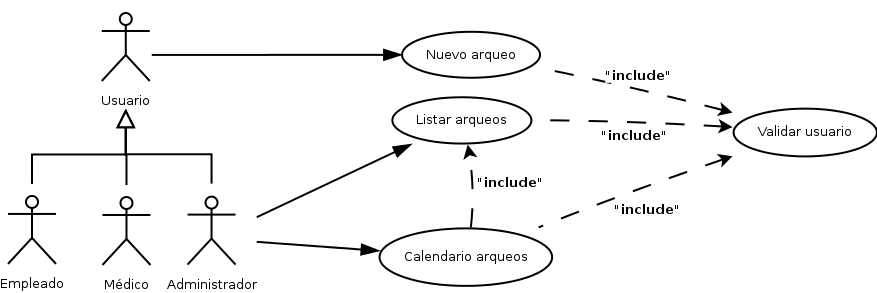
\includegraphics[scale=0.4]{gestionararqueos.png}
  \caption{Diagrama caso de uso. Gestión de arqueos}
  \label{cu1}
\end{figure}
\smallskip
\hrule height 1pt
\smallskip
\textbf{Caso de uso: Nuevo arqueo}
\begin{itemize}\renewcommand{\labelitemi}{$\cdot$}
 \item \textbf{Descripción:} El usuario registra un nuevo arqueo en el sistema.
  \item \textbf{Actores:} Usuario
  \item \textbf{Precondiciones:} Se debe comprobar que en esa fecha no exista un arqueo. Se debe comprobar que el usuario este autenticado en el sistema con el caso de uso Validar usuario.
  \item \textbf{Postcondiciones:} El sistema almacena el arqueo en el sistema.
\end{itemize}
\underline{\textbf{Identificación de escenarios:}}
\begin{itemize}\renewcommand{\labelitemi}{$\circ$}
 \item \textbf{Escenario principal:}
         \begin{enumerate}
          \item El caso de uso se inicia cuando el usuario decide registrar un nuevo arqueo en el sistema.
	\item El sistema muestra la pantalla para la selección de monedas, billetes y boletas.
	   \item El sistema comprueba que los datos introducidos son válidos.
	\item El sistema comprueba que el arqueo es correcto.
 	  \item El sistema almacena el cambio del sistema (auditoria).
          \item El arqueo queda registrado en el sistema.
         \end{enumerate}
  \item \textbf{Escenario alternativos:}\\\\
	4a. El usuario introduce de manera incorrecta los datos.
		\begin{enumerate}
		 \item El sistema muestra el error y pide que se introduzcan de nuevo los datos.
		\end{enumerate}
	5a. El usuario introduce un arqueo inválido.
		\begin{enumerate}
		 \item El sistema muestra el error y da la opción a intentarlo de nuevo o guardar el arqueo inválido.
		\end{enumerate}
          *a. El usuario cancela en cualquier momento el proceso de registro de un nuevo arqueo.
\end{itemize}

\smallskip
\hrule height 1pt
\smallskip
\textbf{Caso de uso: Calendario arqueos}
\begin{itemize}\renewcommand{\labelitemi}{$\cdot$}
 \item \textbf{Descripción:} El administrador decide mostrar el calendario de arqueos.
  \item \textbf{Actores:} Administrador
  \item \textbf{Precondiciones:} Se debe comprobar que el administrador este autenticado en el sistema con el caso de uso Validar usuario.
  \item \textbf{Postcondiciones:} El sistema muestra el calendario con todos los arqueos almacenados en el sistema.
\end{itemize}
\underline{\textbf{Identificación de escenarios:}}
\begin{itemize}\renewcommand{\labelitemi}{$\circ$}
 \item \textbf{Escenario principal:}
         \begin{enumerate}
          \item El caso de uso se inicia cuando el administrador decide mostrar el calendario de arqueos.
	  \item El sistema muestra por pantalla todos los arqueos en el calendario.
         \end{enumerate}
\end{itemize}

\smallskip
\hrule height 1pt
\smallskip
\textbf{Caso de uso: Listar arqueos}
\begin{itemize}\renewcommand{\labelitemi}{$\cdot$}
 \item \textbf{Descripción:} El administrador decide consultar los permisos en el sistema.
  \item \textbf{Actores:} Administrador
  \item \textbf{Precondiciones:} Se debe comprobar que el administrador este autenticado en el sistema con el caso de uso Validar usuario.
  \item \textbf{Postcondiciones:} El sistema muestra por pantalla todos los arqueos.
\end{itemize}
\underline{\textbf{Identificación de escenarios:}}
\begin{itemize}\renewcommand{\labelitemi}{$\circ$}
 \item \textbf{Escenario principal:}
         \begin{enumerate}
          \item El caso de uso se inicia cuando el administrador decide consultar todos los arqueos.
          \item El sistema muestra un listado de todos los arqueos.
          \item El usuario no selecciona un patrón de búsqueda.
          \item El sistema muestra todos los permisos.
         \end{enumerate}
  \item \textbf{Escenario alternativos:}\\
  			3a. El usuario introduce un patrón de búsqueda.
  			\begin{enumerate}
  			\item El sistema muestra los datos acordes a ese patrón de búsqueda.
  			\item El administrador puede seleccionar el patrón de búsqueda cuantas veces desee.
  			\end{enumerate}
          *a. El administrador cancela en cualquier momento la consulta de los arqueos del sistema.
\end{itemize}

\subsection{Requisito funcional: Gestión de permisos}

\begin{itemize}
 \item El administrador podrá registrar un nuevo permiso en el sistema.
 \item El administrador podrá consultar e imprimir el listado de todos los permisos del sistema.
 \item El administrador podrá modificar los permisos del sistema.
 \item El administrador podrá eliminar un permiso en concreto del sistema.
 \item El administrador podrá realizar filtrados de los permisos del sistema.
 \item El usuario podrá consultar sus permisos.
\end{itemize}
\begin{figure}[H]
  \centering
    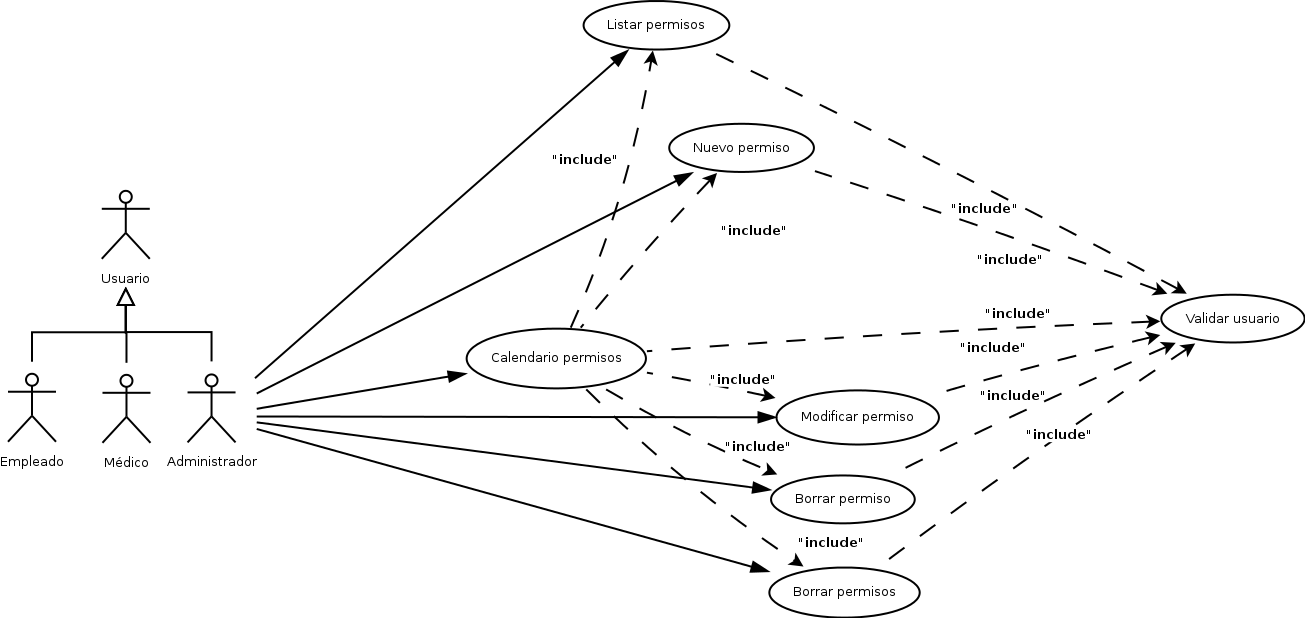
\includegraphics[scale=0.4]{gestionpermisos.png}
  \caption{Diagrama caso de uso. Gestión de permisos}
  \label{cu1}
\end{figure}
\smallskip
\hrule height 1pt
\smallskip
\textbf{Caso de uso: Nuevo permiso}
\begin{itemize}\renewcommand{\labelitemi}{$\cdot$}
 \item \textbf{Descripción:} El empleado registra un nuevo permiso en el sistema.
  \item \textbf{Actores:} Administrador 
  \item \textbf{Precondiciones:} Se debe comprobar que el administrador este autenticado en el sistema con el caso de uso Validar usuario.
  \item \textbf{Postcondiciones:} El sistema almacena el permiso en el sistema.
\end{itemize}
\underline{\textbf{Identificación de escenarios:}}
\begin{itemize}\renewcommand{\labelitemi}{$\circ$}
 \item \textbf{Escenario principal:}
         \begin{enumerate}
          \item El caso de uso se inicia cuando el administrador decide registrar un nuevo permiso en el sistema.
          \item El administrador arrastra al usuario a la fecha del permiso.
	   \item El sistema comprueba que el permiso sea válido.
 	  \item El sistema almacena el cambio del sistema (auditoria).
          \item El permiso queda registrado en el sistema y el permiso aparece en el calendario.
         \end{enumerate}
  \item \textbf{Escenario alternativos:}\\\\
	3a. El aministrador introduce un permiso inválido.
		\begin{enumerate}
		 \item El sistema muestra el error y cancela el registro del permiso.
		\end{enumerate}
          *a. El administrador cancela en cualquier momento el proceso de registro de un nuevo permiso.
\end{itemize}

\smallskip
\hrule height 1pt
\smallskip
\textbf{Caso de uso: Borrar permiso}
\begin{itemize}\renewcommand{\labelitemi}{$\cdot$}
 \item \textbf{Descripción:} El administrador elimina un permiso en concreto en el sistema.
  \item \textbf{Actores:} Administrador 
  \item \textbf{Precondiciones:} Se debe comprobar que el administrador este autenticado en el sistema con el caso de uso Validar usuario.
  \item \textbf{Postcondiciones:} El sistema almacena el permiso modificado en el sistema.
\end{itemize}
\underline{\textbf{Identificación de escenarios:}}
\begin{itemize}\renewcommand{\labelitemi}{$\circ$}
 \item \textbf{Escenario principal:}
         \begin{enumerate}
          \item El caso de uso se inicia cuando el administrador decide eliminar un permiso en el sistema.
	  \item El administrador pulsa en el permiso que desea eliminar.
	  \item El sistema muestra un mensaje de confirmación.
          \item El administrador pulsa SI en el mensaje de confirmación.
 	  \item El sistema almacena el cambio del sistema (auditoria).
          \item El permiso queda eliminado en el sistema y el permiso aparece en el calendario.
         \end{enumerate}
  \item \textbf{Escenario alternativos:}\\\\
		4a. El administrador decide no borrar el permiso.
  			\begin{enumerate}
  			\item El sistema cancela el proceso de eliminación de un permiso.
  			\end{enumerate}
          *a. El administrador cancela en cualquier momento el proceso de eliminación del permiso.
\end{itemize}

\smallskip
\hrule height 1pt
\smallskip
\textbf{Caso de uso: Borrar permisos}
\begin{itemize}\renewcommand{\labelitemi}{$\cdot$}
 \item \textbf{Descripción:} El administrador elimina los permisos de un determinado tipo en concreto en el sistema.
  \item \textbf{Actores:} Administrador 
  \item \textbf{Precondiciones:} Se debe comprobar que el administrador este autenticado en el sistema con el caso de uso Validar usuario.
  \item \textbf{Postcondiciones:} El sistema elimina los permisos de ese tipo en el sistema.
\end{itemize}
\underline{\textbf{Identificación de escenarios:}}
\begin{itemize}\renewcommand{\labelitemi}{$\circ$}
 \item \textbf{Escenario principal:}
         \begin{enumerate}
          \item El caso de uso se inicia cuando el administrador decide eliminar los permisos de un tipo en el sistema.
	  \item El administrador pulsa en el tipo de permiso que desea eliminar.
	  \item El sistema muestra un mensaje de confirmación.
          \item El administrador pulsa SI en el mensaje de confirmación.
 	  \item El sistema almacena el cambio del sistema (auditoria).
          \item Los permisos quedan eliminados en el sistema y el permiso aparece en el calendario.
         \end{enumerate}
  \item \textbf{Escenario alternativos:}\\\\
		4a. El administrador decide no borrar los permisos.
  			\begin{enumerate}
  			\item El sistema cancela el proceso de eliminación de los permisos.
  			\end{enumerate}
          *a. El administrador cancela en cualquier momento el proceso de eliminación de los permisos.
\end{itemize}

\smallskip
\hrule height 1pt
\smallskip
\textbf{Caso de uso: Calendario permisos}
\begin{itemize}\renewcommand{\labelitemi}{$\cdot$}
 \item \textbf{Descripción:} El administrador decide mostrar el calendario de permisos.
  \item \textbf{Actores:} Administrador
  \item \textbf{Precondiciones:} Se debe comprobar que el administrador este autenticado en el sistema con el caso de uso Validar usuario.
  \item \textbf{Postcondiciones:} El sistema muestra el calendario con todos los permisos almacenados en el sistema.
\end{itemize}
\underline{\textbf{Identificación de escenarios:}}
\begin{itemize}\renewcommand{\labelitemi}{$\circ$}
 \item \textbf{Escenario principal:}
         \begin{enumerate}
          \item El caso de uso se inicia cuando el administrador decide mostrar el calendario de permisos.
	  \item El sistema muestra por pantalla todos los permisos en el calendario.
         \end{enumerate}
\end{itemize}

\smallskip
\hrule height 1pt
\smallskip
\textbf{Caso de uso: Listar permisos}
\begin{itemize}\renewcommand{\labelitemi}{$\cdot$}
 \item \textbf{Descripción:} El administrador decide consultar los permisos en el sistema.
  \item \textbf{Actores:} Administrador, Cliente
  \item \textbf{Precondiciones:} Se debe comprobar que el administrador este autenticado en el sistema con el caso de uso Validar usuario. Si el usuario no es administrador sólo podrá listar sus propios permisos.
  \item \textbf{Postcondiciones:} El sistema muestra por pantalla todos los permisos.
\end{itemize}
\underline{\textbf{Identificación de escenarios:}}
\begin{itemize}\renewcommand{\labelitemi}{$\circ$}
 \item \textbf{Escenario principal:}
         \begin{enumerate}
          \item El caso de uso se inicia cuando el administrador decide consultar todos los permisos.
          \item El sistema muestra un listado de todos los permisos.
          \item El usuario no selecciona un patrón de búsqueda.
          \item El sistema muestra todos los permisos.
         \end{enumerate}
  \item \textbf{Escenario alternativos:}\\
  			3a. El administrador introduce un patrón de búsqueda.
  			\begin{enumerate}
  			\item El sistema muestra los datos acordes a ese patrón de búsqueda.
  			\item El administrador puede seleccionar el patrón de búsqueda cuantas veces desee.
  			\end{enumerate}
          *a. El usuario cancela en cualquier momento la consulta de los permisos del sistema.
\end{itemize}

\section{Requisitos de información}

En este apartado estudiaremos todos los datos referentes al diseño del esquema conceptual: Se identificarán las clases, atributos, relaciones, restricciones adicionales y reglas de derivación necesarias.

\clearpage

\subsection{Modelo conceptual de datos}
\begin{figure}[H]
  \centering
    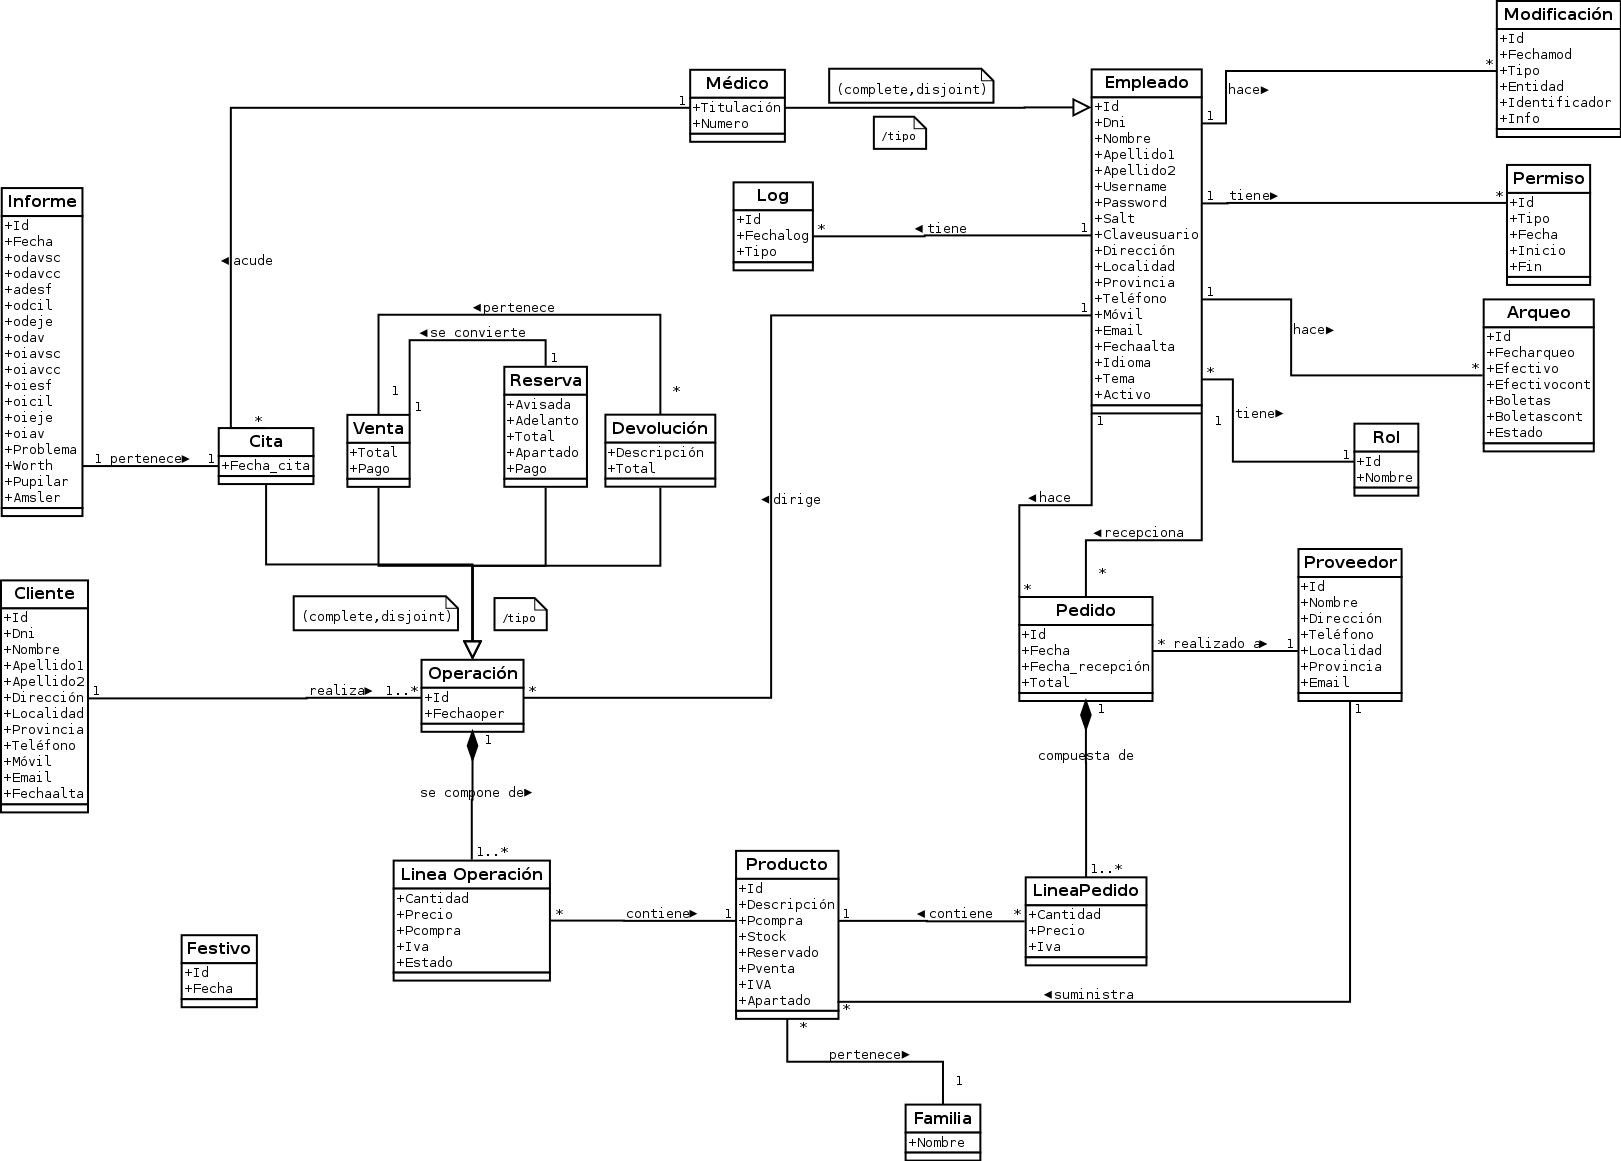
\includegraphics[angle=-90,scale=0.34]{UML.png}
  \caption{Modelo conceptual de datos.}
  \label{uml}
\end{figure}

\section{Modelo comportamiento del sistema}

\subsection{Diagramas de secuencia de sistemas}

Una vez descritos los casos de uso, nos ponemos manos a la obra para realizar los diferentes diagramas de secuencia. En esta fase de análisis describiremos los diagramas de manera muy simplificada ya que estos se estudiarán más a fondo en la fase de diseño.\\
Sólo nos centraremos en los diagramas que tengan relevancia ya que muchos de ellos son muy similares.

\subsubsection{Gestión de entradas y salidas del sistema}
\begin{figure}[!htb]
  \centering
    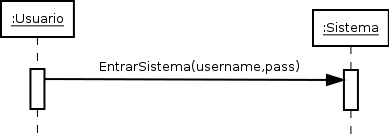
\includegraphics[scale=0.5]{aentrarsistema.png}
  \caption{Diagrama de secuencia - Caso de uso: Entrada al sistema }
  \label{a}
\end{figure}

\begin{figure}[!htb]
  \centering
    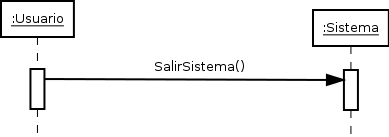
\includegraphics[scale=0.5]{asalirsistema.png}
  \caption{Diagrama de secuencia - Caso de uso: Salida del sistema }
  \label{a}
\end{figure}

\begin{figure}[!htb]
  \centering
    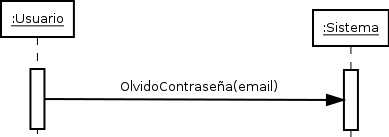
\includegraphics[scale=0.5]{aolvidocontrasena.png}
  \caption{Diagrama de secuencia - Caso de uso: Olvido contraseña  }
  \label{a}
\end{figure}

\begin{figure}[!htb]
  \centering
    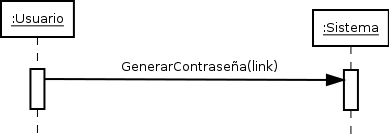
\includegraphics[scale=0.5]{agenerarcontrasena.png}
  \caption{Diagrama de secuencia - Caso de uso: Generar contraseña  }
  \label{a}
\end{figure}

\clearpage
\subsubsection{Gestión de clientes}
\begin{figure}[!htb]
  \centering
    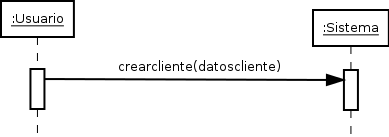
\includegraphics[scale=0.5]{aregistrarcliente.png}
  \caption{Diagrama de secuencia - Caso de uso: Registrar cliente }
  \label{a}
\end{figure}

\begin{figure}[!htb]
  \centering
    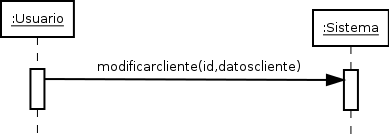
\includegraphics[scale=0.5]{aeditarcliente.png}
  \caption{Diagrama de secuencia - Caso de uso: Modificar cliente }
  \label{a}
\end{figure}

\begin{figure}[!htb]
  \centering
    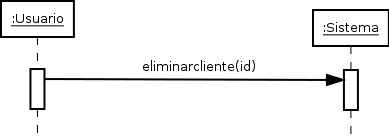
\includegraphics[scale=0.5]{aborrarcliente.png}
  \caption{Diagrama de secuencia - Caso de uso: Borrar cliente   }
  \label{a}
\end{figure}

\begin{figure}[!htb]
  \centering
    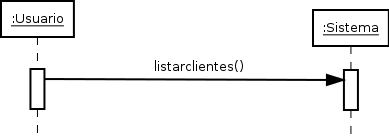
\includegraphics[scale=0.5]{acliente.png}
  \caption{Diagrama de secuencia - Caso de uso: Listar clientes   }
  \label{a}
\end{figure}

\begin{figure}[!htb]
  \centering
    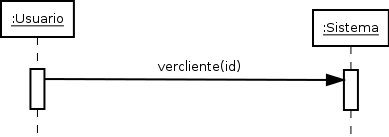
\includegraphics[scale=0.5]{avercliente.png}
  \caption{Diagrama de secuencia - Caso de uso: Ver cliente   }
  \label{a}
\end{figure}

\vspace{15mm}
\subsubsection{Gestión de ventas}
\begin{figure}[!htb]
  \centering
    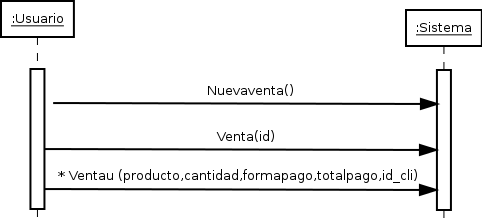
\includegraphics[scale=0.5]{aregistarventa.png}
  \caption{Diagrama de secuencia - Caso de uso: Nueva venta }
  \label{a}
\end{figure}

\begin{figure}[!htb]
  \centering
    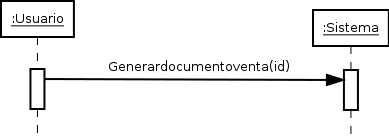
\includegraphics[scale=0.5]{agenerarfactura.png}
  \caption{Diagrama de secuencia - Caso de uso: Generar documento venta }
  \label{a}
\end{figure}

\begin{figure}[!htb]
  \centering
    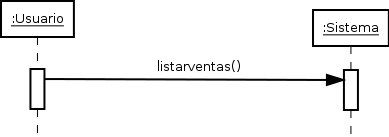
\includegraphics[scale=0.5]{aventa.png}
  \caption{Diagrama de secuencia - Caso de uso: Listar ventas   }
  \label{a}
\end{figure}

\begin{figure}[!htb]
  \centering
    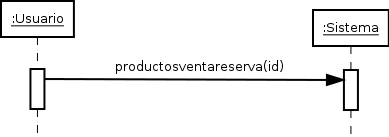
\includegraphics[scale=0.5]{averproductosventa.png}
  \caption{Diagrama de secuencia - Caso de uso: Ver productos venta }
  \label{a}
\end{figure}

\newpage
\subsubsection{Gestión de devoluciones}
\begin{figure}[!htb]
  \centering
    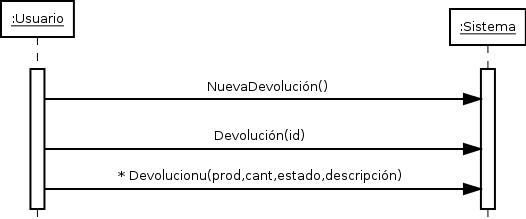
\includegraphics[scale=0.5]{aregistardevolucion.png}
  \caption{Diagrama de secuencia - Caso de uso: Nueva devolución }
  \label{a}
\end{figure}

\begin{figure}[!htb]
  \centering
    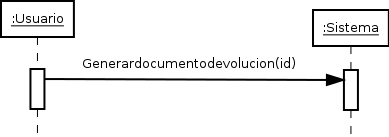
\includegraphics[scale=0.5]{agenerardocumento.png}
  \caption{Diagrama de secuencia - Caso de uso: Generar documento devolución}
  \label{a}
\end{figure}

\begin{figure}[!htb]
  \centering
    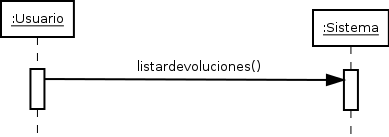
\includegraphics[scale=0.5]{adevolucion.png}
  \caption{Diagrama de secuencia - Caso de uso: Listar devoluciones }
  \label{a}
\end{figure}

\begin{figure}[!htb]
  \centering
    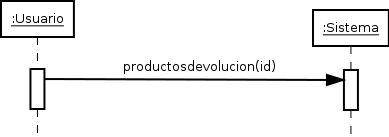
\includegraphics[scale=0.5]{averproductosdevueltos.png}
  \caption{Diagrama de secuencia - Caso de uso: Ver productos devolución  }
  \label{a}
\end{figure}

\newpage
\subsubsection{Gestión de reservas}
\begin{figure}[!htb]
  \centering
    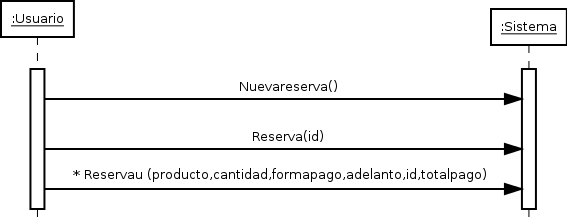
\includegraphics[scale=0.5]{aregistarreserva.png}
  \caption{Diagrama de secuencia - Caso de uso: Nueva reserva }
  \label{a}
\end{figure}

\begin{figure}[!htb]
  \centering
    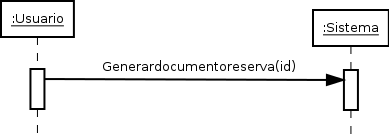
\includegraphics[scale=0.5]{agenerardocumentoreserva.png}
  \caption{Diagrama de secuencia - Caso de uso: Generar documento reserva }
  \label{a}
\end{figure}

\begin{figure}[!htb]
  \centering
    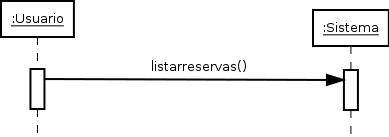
\includegraphics[scale=0.5]{areserva.png}
  \caption{Diagrama de secuencia - Caso de uso: Listar reservas   }
  \label{a}
\end{figure}

\begin{figure}[!htb]
  \centering
    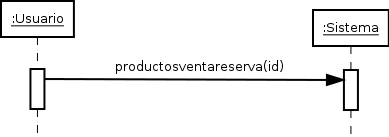
\includegraphics[scale=0.5]{averproductosreserva.png}
  \caption{Diagrama de secuencia - Caso de uso: Ver productos reserva  }
  \label{a}
\end{figure}

\begin{figure}[!htb]
  \centering
    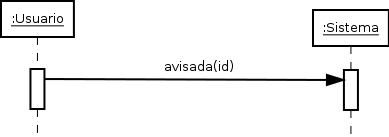
\includegraphics[scale=0.5]{aavisada.png}
  \caption{Diagrama de secuencia - Caso de uso: Avisar reserva   }
  \label{a}
\end{figure}

\begin{figure}[!htb]
  \centering
    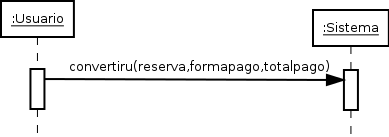
\includegraphics[scale=0.5]{aconvertir.png}
  \caption{Diagrama de secuencia - Caso de uso: Convertir a venta  }
  \label{a}
\end{figure}

\newpage
\subsubsection{Gestión de citas e informes}
\begin{figure}[!htb]
  \centering
    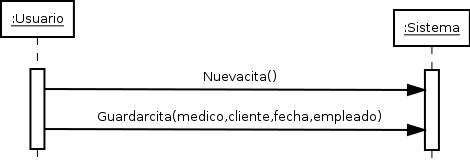
\includegraphics[scale=0.5]{aregistrarcita.png}
  \caption{Diagrama de secuencia - Caso de uso: Nueva cita }
  \label{a}
\end{figure}

\begin{figure}[!htb]
  \centering
    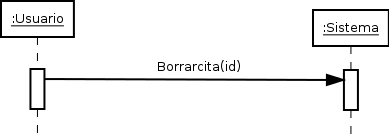
\includegraphics[scale=0.5]{aborrarcita.png}
  \caption{Diagrama de secuencia - Caso de uso: Borrar cita   }
  \label{a}
\end{figure}

\begin{figure}[!htb]
  \centering
    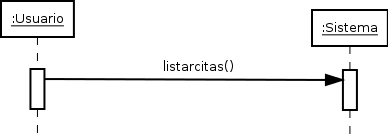
\includegraphics[scale=0.5]{acita.png}
  \caption{Diagrama de secuencia - Caso de uso: Listar citas   }
  \label{a}
\end{figure}

\begin{figure}[!htb]
  \centering
    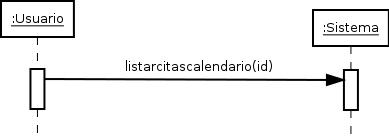
\includegraphics[scale=0.5]{acitas.png}
  \caption{Diagrama de secuencia - Caso de uso: Calendario citas   }
  \label{a}
\end{figure}

\begin{figure}[!htb]
  \centering
    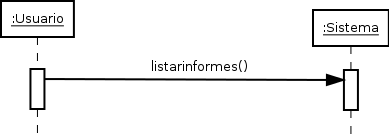
\includegraphics[scale=0.5]{ainforme.png}
  \caption{Diagrama de secuencia - Caso de uso: Listar informes   }
  \label{a}
\end{figure}

\begin{figure}[!htb]
  \centering
    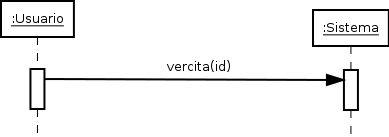
\includegraphics[scale=0.5]{avercita.png}
  \caption{Diagrama de secuencia - Caso de uso: Ver cita   }
  \label{a}
\end{figure}

\begin{figure}[!htb]
  \centering
    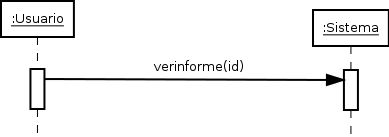
\includegraphics[scale=0.5]{averinforme.png}
  \caption{Diagrama de secuencia - Caso de uso: Ver informe   }
  \label{a}
\end{figure}

\begin{figure}[!htb]
  \centering
    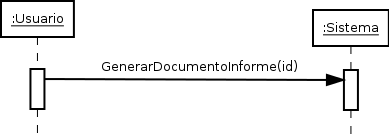
\includegraphics[scale=0.5]{agenerardocumentoinforme.png}
  \caption{Diagrama de secuencia - Caso de uso: Generar documento informe   }
  \label{a}
\end{figure}

\begin{figure}[!htb]
  \centering
    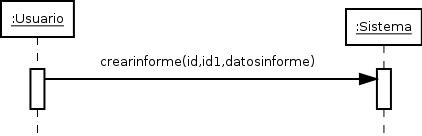
\includegraphics[scale=0.5]{agenerarinformeconcita.png}
  \caption{Diagrama de secuencia - Caso de uso: Nuevo informe con cita   }
  \label{a}
\end{figure}

\begin{figure}[!htb]
  \centering
    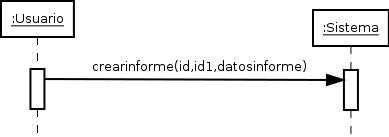
\includegraphics[scale=0.5]{agenerarinformesincita.png}
  \caption{Diagrama de secuencia - Caso de uso: Nuevo informe sin cita  }
  \label{a}
\end{figure}

\clearpage
\subsubsection{Gestión de pedidos}
\begin{figure}[!htb]
  \centering
    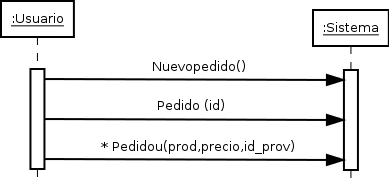
\includegraphics[scale=0.5]{aregistrarpedido.png}
  \caption{Diagrama de secuencia - Caso de uso: Nuevo pedido }
  \label{a}
\end{figure}

\begin{figure}[!htb]
  \centering
    \includegraphics[scale=0.5]{agenerardocumentopedido.png}
  \caption{Diagrama de secuencia - Caso de uso: Generar documento pedido }
  \label{a}
\end{figure}

\begin{figure}[!htb]
  \centering
    \includegraphics[scale=0.5]{apedido.png}
  \caption{Diagrama de secuencia - Caso de uso: Listar pedidos }
  \label{a}
\end{figure}

\begin{figure}[!htb]
  \centering
    \includegraphics[scale=0.5]{averproductospedido.png}
  \caption{Diagrama de secuencia - Caso de uso: Ver productos pedido }
  \label{a}
\end{figure}

\begin{figure}[!htb]
  \centering
    \includegraphics[scale=0.5]{arecepcionarpedido.png}
  \caption{Diagrama de secuencia - Caso de uso: Recepcionar pedido }
  \label{a}
\end{figure}

\subsubsection{Gestión de usuarios}
Se han omitido algunos diagramas ya que son similares a los anteriores.

\begin{figure}[!htb]
  \centering
    \includegraphics[scale=0.5]{aregistrarempleado.png}
  \caption{Diagrama de secuencia - Caso de uso: Registrar empleado  }
  \label{a}
\end{figure}

\begin{figure}[!htb]
  \centering
    \includegraphics[scale=0.5]{aregistrarmedico.png}
  \caption{Diagrama de secuencia - Caso de uso: Registrar médico   }
  \label{a}
\end{figure}

\begin{figure}[!htb]
  \centering
    \includegraphics[scale=0.5]{averconexiones.png}
  \caption{Diagrama de secuencia - Caso de uso: Listar conexiones   }
  \label{a}
\end{figure}

\begin{figure}[!htb]
  \centering
    \includegraphics[scale=0.5]{avercambios.png}
  \caption{Diagrama de secuencia - Caso de uso: Listar cambios  }
  \label{a}
\end{figure}
 
\clearpage
\subsubsection{Gestión de permisos}
\begin{figure}[!htb]
  \centering
    \includegraphics[scale=0.5]{aregistrarpermiso.png}
  \caption{Diagrama de secuencia - Caso de uso: Nuevo permiso }
  \label{a}
\end{figure}

\begin{figure}[!htb]
  \centering
    \includegraphics[scale=0.5]{aborrarpermiso.png}
  \caption{Diagrama de secuencia - Caso de uso: Borrar permiso }
  \label{a}
\end{figure}

\begin{figure}[!htb]
  \centering
    \includegraphics[scale=0.5]{aborrarpermisos.png}
  \caption{Diagrama de secuencia - Caso de uso: Borrar permisos }
  \label{a}
\end{figure}

\begin{figure}[!htb]
  \centering
    \includegraphics[scale=0.5]{amodificarpermiso.png}
  \caption{Diagrama de secuencia - Caso de uso: Modificar permiso }
  \label{a}
\end{figure}

\begin{figure}[!htb]
  \centering
    \includegraphics[scale=0.5]{alistarpermisos.png}
  \caption{Diagrama de secuencia - Caso de uso: Listar permisos }
  \label{a}
\end{figure}

\clearpage

\begin{figure}[!htb]
  \centering
    \includegraphics[scale=0.5]{acalendariopermisos.png}
  \caption{Diagrama de secuencia - Caso de uso: Calendario permisos }
  \label{a}
\end{figure}

\subsubsection{Gestión de festivos}
\begin{figure}[!htb]
  \centering
    \includegraphics[scale=0.5]{aregistrarfestivo.png}
  \caption{Diagrama de secuencia - Caso de uso: Registrar festivo }
  \label{a}
\end{figure}

\begin{figure}[!htb]
  \centering
    \includegraphics[scale=0.5]{aborrarfestivo.png}
  \caption{Diagrama de secuencia - Caso de uso: Borrar festivo }
  \label{a}
\end{figure}

\begin{figure}[!htb]
  \centering
    \includegraphics[scale=0.5]{afestivo.png}
  \caption{Diagrama de secuencia - Caso de uso: Listar festivos }
  \label{a}
\end{figure}

\begin{figure}[!htb]
  \centering
    \includegraphics[scale=0.5]{afestivos.png}
  \caption{Diagrama de secuencia - Caso de uso: Calendario festivos }
  \label{a}
\end{figure}
\clearpage

\subsubsection{Gestión de arqueos}
\begin{figure}[!htb]
  \centering
    \includegraphics[scale=0.5]{anuevoarqueo.png}
  \caption{Diagrama de secuencia - Caso de uso: Nuevo arqueo }
  \label{a}
\end{figure}

\begin{figure}[!htb]
  \centering
    \includegraphics[scale=0.5]{aarqueos.png}
  \caption{Diagrama de secuencia - Caso de uso: Listar arqueos }
  \label{a}
\end{figure}

\begin{figure}[!htb]
  \centering
    \includegraphics[scale=0.5]{aarqueoscalendario.png}
  \caption{Diagrama de secuencia - Caso de uso: Calendario arqueos }
  \label{a}
\end{figure}

\subsubsection{Estadísticas}
\begin{figure}[!htb]
  \centering
    \includegraphics[scale=0.5]{aestadistica.png}
  \caption{Diagrama de secuencia - Caso de uso: Estadísticas }
  \label{a}
\end{figure}

\begin{figure}[!htb]
  \centering
    \includegraphics[scale=0.5]{aestadistica1.png}
  \caption{Diagrama de secuencia - Caso de uso: Estadísticas empleado }
  \label{a}
\end{figure}

\newpage
\subsection{Contratos de las operaciones}

En este apartado describiremos el comportamiento que debe tener el sistema para cada diagrama descrito anteriormente. Sólo nos centraremos en lo que hace el sistema en cada operación pero no como lo hace. Para que no existan confusiones entre datos del sistema y datos proporcionados usaremos la notación W para datos proporcionados al sistema. Describiremos los contratos de las operaciones de forma clara haciendo uso de la siguiente plantilla estudiada en ingeniería del software:

\begin{table}[h]
\begin{tabular}{|m{6.0cm}|m{10.0cm}|}
\hline\hline                        %inserts double horizontal lines
\multicolumn{2}{|>{\columncolor[gray]{0.93}}c|}{\textbf{Plantilla de un contrato}  } \\
\hline
\hline                  % inserts single horizontal line
\textbf{Nombre operación} & Signatura de la operación \\ % inserting body of the table
\hline
\textbf{Responsabilidades} & Descripción informal del propósito de la operación \\ % inserting body of the table
\hline
\textbf{Referencias cruzadas(opcional)} & Casos de uso en los que puede tener lugar la operación \\ % inserting body of the table
\hline
\textbf{Precondiciones} &  Suposiciones relevantes sobre el estado del sistema o de los objetos del modelo conceptual, ante de ejecutar la operación. Suposiciones no triviales. \\ % inserting body of the table
\hline
\textbf{Postcondiciones} & Estado de los objetos del modelo conceptual después de que se ejecute la operación \\ % inserting body of the table
\hline
\end{tabular}
\caption{Plantilla de un contrato} % title of Table
\end{table}

Ahora describiremos los contratos de las operaciones para los diagramas de secuencia descritos anteriormente.

\begin{table}[h]
\begin{tabular}{|m{4cm}|m{12cm}|}
\hline\hline                        %inserts double horizontal lines
\multicolumn{2}{|>{\columncolor[gray]{0.93}}c|}{\textbf{Plantilla contrato: Entrar al sistema}  } \\
\hline
\hline                  % inserts single horizontal line
\textbf{Nombre operación} & EntrarSistema(username,pass) \\ % inserting body of the table
\hline
\textbf{Responsabilidades} & Realizar la autenticación del usuario en el sistema \\ % inserting body of the table
\hline
\textbf{Referencias cruzadas} & Caso de uso \textbf{Entrar al sistema} \\ % inserting body of the table
\hline
\textbf{Precondiciones} & \begin{itemize}\item Existe un usuario con w\_username = username. \item El w\_pass debe coincidir con pass. \end{itemize}\\
\hline
\textbf{Postcondiciones} & \begin{itemize}\item Se creó una instancia de Log(creación de objeto). \item El identificador del Log se verá incrementado en 1. \item Se asignó fechalog: fechaactual y tipo: Entrada. \item Se asoció el usuario autenticado con el objeto Log.\item El sistema concede la entrada al usuario en el sistema y muestra la pantalla principal.\end{itemize}\\ % inserting body of the table
\hline
\end{tabular}
\caption{Operación : \textbf{EntrarSistema(username,pass)}} % title of Table
\end{table}
\clearpage

\begin{table}[!h]
\begin{tabular}{|m{4cm}|m{12cm}|}
\hline\hline                        %inserts double horizontal lines
\multicolumn{2}{|>{\columncolor[gray]{0.93}}c|}{\textbf{Plantilla contrato: Salir del sistema}  } \\
\hline
\hline                  % inserts single horizontal line
\textbf{Nombre operación} & SalirSistema() \\ % inserting body of the table
\hline
\textbf{Responsabilidades} & Realizar la salida del usuario del sistema \\ % inserting body of the table
\hline
\textbf{Referencias cruzadas} & Caso de uso \textbf{Salir del sistema} \\ % inserting body of the table
\hline
\textbf{Precondiciones} & \begin{itemize}\item Existe un usuario autenticado en el sistema.\end{itemize}\\
\hline
\textbf{Postcondiciones} & \begin{itemize}\item Se creó una instancia de Log(creación de objeto). \item El identificador del Log se verá incrementado en 1. \item Se asignó fechalog: fechaactual y tipo: Salida. \item Se asoció el usuario autenticado con el objeto Log.\item El sistema concede la salida al usuario del sistema.\end{itemize}\\ % inserting body of the table
\hline
\end{tabular}
\caption{Operación : \textbf{SalirSistema()}} % title of Table
\end{table}

\begin{table}[!h]
\begin{tabular}{|m{4cm}|m{12cm}|}
\hline\hline                        %inserts double horizontal lines
\multicolumn{2}{|>{\columncolor[gray]{0.93}}c|}{\textbf{Plantilla contrato: Olvido contraseña}  } \\
\hline
\hline                  % inserts single horizontal line
\textbf{Nombre operación} & Olvidocontraseña(email) \\ % inserting body of the table
\hline
\textbf{Responsabilidades} & Enviar enlace para generar nueva contraseña \\ % inserting body of the table
\hline
\textbf{Referencias cruzadas} & Caso de uso \textbf{Olvido contraseña} \\ % inserting body of the table
\hline
\textbf{Precondiciones} & \begin{itemize}\item Existe un usuario en el sistema con w\_email = email. \end{itemize}\\
\hline
\textbf{Postcondiciones} & \begin{itemize}\item El sistema envía por correo un link de reestablecimiento de contraseña. \end{itemize}\\ % inserting body of the table
\hline
\end{tabular}
\caption{Operación : \textbf{OlvidoContraseña(email)}} % title of Table
\end{table}

\begin{table}[!h]
\begin{tabular}{|m{4cm}|m{12cm}|}
\hline\hline                        %inserts double horizontal lines
\multicolumn{2}{|>{\columncolor[gray]{0.93}}c|}{\textbf{Plantilla contrato: Generar contraseña}  } \\
\hline
\hline                  % inserts single horizontal line
\textbf{Nombre operación} & GenerarContraseña(link) \\ % inserting body of the table
\hline
\textbf{Responsabilidades} & Generar una nueva contraseña aleatoria para el usuario. \\ % inserting body of the table
\hline
\textbf{Referencias cruzadas} & Caso de uso \textbf{Generar contraseña} \\ % inserting body of the table
\hline
\textbf{Precondiciones} & \begin{itemize}\item Existe un usuario con w\_claveusuario = claveusuario. \end{itemize}\\
\hline
\textbf{Postcondiciones} & \begin{itemize}\item El sistema genera y almacena una nueva contraseña aleatoria para el usuario. \item El sistema manda un correo al usuario indicando la nueva contraseña.\end{itemize}\\ % inserting body of the table
\hline
\end{tabular}
\caption{Operación : \textbf{GenerarContraseña(link)}} % title of Table
\end{table}

\newpage
\begin{table}[h]
\begin{tabular}{|m{4cm}|m{12cm}|}
\hline\hline                        %inserts double horizontal lines
\multicolumn{2}{|>{\columncolor[gray]{0.93}}c|}{\textbf{Plantilla contrato: Registrar Cliente}  } \\
\hline
\hline                  % inserts single horizontal line
\textbf{Nombre operación} & Crearcliente(datoscliente) \\ % inserting body of the table
\hline
\textbf{Responsabilidades} & Almacenar a un cliente en el sistema. \\ % inserting body of the table
\hline
\textbf{Referencias cruzadas} & Caso de uso \textbf{Registrar cliente} \\ % inserting body of the table
\hline
\textbf{Precondiciones} & \begin{itemize}\item Los datos insertados datoscliente son válidos. \end{itemize}\\
\hline
\textbf{Postcondiciones} & \begin{itemize}\item Se creó una instancia de Cliente(creación de objeto).\item El identificador del cliente se verá incrementado en 1. \item Los datoscliente se asignan al nuevo cliente.\item Se creó una instancia de Modificación(creación de objeto). \item El identificador de Modificación se verá incrementado en 1. \item Se asignó fechamod: fechaactual, tipo: Insercion, Entidad: Cliente, Identificador: id\_cli. \item Se asoció el usuario autenticado con el objeto Modificación. \end{itemize}\\ % inserting body of the table
\hline
\end{tabular}
\caption{Operación : \textbf{Crearcliente(datoscliente)}} % title of Table
\end{table}

\begin{table}[h]
\begin{tabular}{|m{4cm}|m{12cm}|}
\hline\hline                        %inserts double horizontal lines
\multicolumn{2}{|>{\columncolor[gray]{0.93}}c|}{\textbf{Plantilla contrato: Modificar Cliente}  } \\
\hline
\hline                  % inserts single horizontal line
\textbf{Nombre operación} & Modificarcliente(id,datoscliente) \\ % inserting body of the table
\hline
\textbf{Responsabilidades} & Almacenar en el sistema la modificación de los datos de un cliente \\ % inserting body of the table
\hline
\textbf{Referencias cruzadas} & Caso de uso \textbf{Modificar cliente} \\ % inserting body of the table
\hline
\textbf{Precondiciones} & \begin{itemize}\item Los datos insertados datoscliente son válidos.\item Existe un cliente almacenado con w\_id = id.\end{itemize}\\
\hline
\textbf{Postcondiciones} & \begin{itemize} \item Se creó una instancia de Modificación(creación de objeto). \item El identificador de Modificación se verá incrementado en 1. \item Se asignó fechamod: fechaactual, tipo: Modificación, Entidad: Cliente, Identificador: id\_cli. info: datos-antes datos-después\item Se asoció el usuario autenticado con el objeto Modificación.\item Los datoscliente se asignan al cliente visualizado.  \end{itemize}\\ % inserting body of the table
\hline
\end{tabular}
\caption{Operación : \textbf{Modificarcliente(id,datoscliente)}} % title of Table
\end{table}

\begin{table}[h]
\begin{tabular}{|m{4cm}|m{12cm}|}
\hline\hline                        %inserts double horizontal lines
\multicolumn{2}{|>{\columncolor[gray]{0.93}}c|}{\textbf{Plantilla contrato: Borrar Cliente}  } \\
\hline
\hline                  % inserts single horizontal line
\textbf{Nombre operación} & Eliminarcliente(id) \\ % inserting body of the table
\hline
\textbf{Responsabilidades} & Eliminar a un cliente del sistema \\ % inserting body of the table
\hline
\textbf{Referencias cruzadas} & Caso de uso \textbf{Borrar cliente} \\ % inserting body of the table
\hline
\textbf{Precondiciones} & \begin{itemize}\item Existe un cliente almacenado con w\_id = id.\item El cliente no esta asociado a ninguna operación.\end{itemize}\\
\hline
\textbf{Postcondiciones} & \begin{itemize} \item Se creó una instancia de Modificación(creación de objeto). \item El identificador de Modificación se verá incrementado en 1. \item Se asignó fechamod: fechaactual, tipo: Eliminación, Entidad: Cliente, Identificador: id\_cli. \item Se asoció el usuario autenticado con el objeto Modificación. \item Se elimina al cliente visualizado del sistema.\end{itemize}\\ % inserting body of the table
\hline
\end{tabular}
\caption{Operación : \textbf{Eliminarcliente(id)}} % title of Table
\end{table}

\begin{table}[!h]
\begin{tabular}{|m{4cm}|m{12cm}|}
\hline\hline                        %inserts double horizontal lines
\multicolumn{2}{|>{\columncolor[gray]{0.93}}c|}{\textbf{Plantilla contrato: Listar Clientes}  } \\
\hline
\hline                  % inserts single horizontal line
\textbf{Nombre operación} & Listarclientes() \\ % inserting body of the table
\hline
\textbf{Responsabilidades} & Listar todos los clientes del sistema \\ % inserting body of the table
\hline
\textbf{Referencias cruzadas} & Caso de uso \textbf{Listar clientes} \\ % inserting body of the table
\hline
\textbf{Postcondiciones} & \begin{itemize} \item Se muestran por pantalla todos los clientes del sistema. \end{itemize}\\ % inserting body of the table
\hline
\end{tabular}
\caption{Operación : \textbf{Listarclientes()}} % title of Table
\end{table}

\begin{table}[!h]
\begin{tabular}{|m{4cm}|m{12cm}|}
\hline\hline                        %inserts double horizontal lines
\multicolumn{2}{|>{\columncolor[gray]{0.93}}c|}{\textbf{Plantilla contrato: Ver Cliente}  } \\
\hline
\hline                  % inserts single horizontal line
\textbf{Nombre operación} & Vercliente(id) \\ % inserting body of the table
\hline
\textbf{Responsabilidades} & Ver la información del cliente del sistema \\ % inserting body of the table
\hline
\textbf{Referencias cruzadas} & Caso de uso \textbf{Ver cliente} \\ % inserting body of the table
\hline
\textbf{Precondiciones} & \begin{itemize}\item Existe un cliente almacenado con w\_id = id.\end{itemize}\\
\hline
\textbf{Postcondiciones} & \begin{itemize} \item Se muestran por pantalla todos los datos referentes al cliente. \end{itemize}\\ % inserting body of the table
\hline
\end{tabular}
\caption{Operación : \textbf{Vercliente(id)}} % title of Table
\end{table}

\begin{table}[!h]
\begin{tabular}{|m{4cm}|m{12cm}|}
\hline\hline                        %inserts double horizontal lines
\multicolumn{2}{|>{\columncolor[gray]{0.93}}c|}{\textbf{Plantilla contrato: Nueva venta}  } \\
\hline
\hline                  % inserts single horizontal line
\textbf{Nombre operación} & NuevaVenta() \\ % inserting body of the table
\hline
\textbf{Responsabilidades} & Obtener clientes para que se puedan seleccionar.\\ % inserting body of the table
\hline
\textbf{Referencias cruzadas} & Caso de uso \textbf{Nueva Venta} \\ % inserting body of the table
\hline
\textbf{Postcondiciones} & \begin{itemize}  \item Se muestran por pantalla todos los clientes para una nueva venta.\end{itemize}\\ % inserting body of the table
\hline
\end{tabular}
\caption{Operación : \textbf{NuevaVenta()}} % title of Table
\end{table}

\begin{table}[!h]
\begin{tabular}{|m{4cm}|m{12cm}|}
\hline\hline                        %inserts double horizontal lines
\multicolumn{2}{|>{\columncolor[gray]{0.93}}c|}{\textbf{Plantilla contrato: Nueva venta}  } \\
\hline
\hline                  % inserts single horizontal line
\textbf{Nombre operación} & Venta(id) \\ % inserting body of the table
\hline
\textbf{Responsabilidades} & Obtener la lista de productos para que se puedan seleccionar\\ % inserting body of the table
\hline
\textbf{Referencias cruzadas} & Caso de uso \textbf{Nueva Venta} \\ % inserting body of the table
\hline
\textbf{Postcondiciones} & 
\begin{itemize}
\item Se muestra por pantalla el cliente y la lista de productos para que se puedan seleccionar.
\end{itemize}\\ % inserting body of the table
\hline
\end{tabular}
\caption{Operación : \textbf{Venta(id)}} % title of Table
\end{table}


 \begin{table}[!h]
\begin{tabular}{|m{4cm}|m{12cm}|}
\hline\hline                        %inserts double horizontal lines
\multicolumn{2}{|>{\columncolor[gray]{0.93}}c|}{\textbf{Plantilla contrato: Nueva venta}  } \\
\hline
\hline                  % inserts single horizontal line
\textbf{Nombre operación} & Ventau(producto,cant,formapago,totalpago,rc) \\ % inserting body of the table
\hline
\textbf{Responsabilidades} & Almacenar en el sistema los productos de una venta \\ % inserting body of the table
\hline
\textbf{Referencias cruzadas} & Caso de uso \textbf{Nueva Venta} \\ % inserting body of the table
\hline
\textbf{Precondiciones} & \begin{itemize}\item Los productos y cantidades son válidos\end{itemize}\\
\hline
\textbf{Postcondiciones} & 
\begin{itemize}
\item Se creó una instancia de la superclase Operación (creación de objeto).
\item Se asignó fecha:fechaactual. 
\item El identificador de Operación se verá incrementado en 1. 
\item Se asoció el usuario y el cliente con la operación.
\item Se creó una instancia de la subclase Venta(creación de objeto).
\item El identificador de la venta se verá incrementado en 1. 
\item Se crean instancias de LineaOperación (creación de objetos).
\item Se asignan cantidad,precio-venta,precio-compra,iva de cada producto a las lineas de operación.
\item Se asocian los productos con las lineas de operación.
\item Se decrementan los stocks de los productos implicados.
\item Se asocian las LineasOperacion con la venta.
\item Se actualiza el total, totalpago y formapago de la venta.
\item Se crean instancias de Modificación(creación de objetos). 
\item El identificador de Modificación se verá incrementado en 1. 
\item Se asignó fechamod: fechaactual, tipo: Modificación, Entidad: Producto, Identificador: id\_prod info:stockanterior stockactual. 
\item Se asoció el usuario autenticado con el objeto Modificación.
\item Se crea instancia de Modificación(creación de objetos). 
\item El identificador de Modificación se verá incrementado en 1. 
\item Se asignó fechamod: fechaactual, tipo: Inserción, Entidad: Venta, info: total. 
\item Se asoció el usuario autenticado con el objeto Modificación.
\end{itemize}\\ % inserting body of the table
\hline
\end{tabular}
\caption{Operación : \textbf{Ventau(producto,cant,formapago,totalpago,rc)}} % title of Table
\end{table}
\begin{table}[!h]
\begin{tabular}{|m{4cm}|m{12cm}|}
\hline\hline                        %inserts double horizontal lines
\multicolumn{2}{|>{\columncolor[gray]{0.93}}c|}{\textbf{Plantilla contrato: Generar documento venta}  } \\
\hline
\hline                  % inserts single horizontal line
\textbf{Nombre operación} & Generardocumentoventa(id) \\ % inserting body of the table
\hline
\textbf{Responsabilidades} & Generar el documento de una venta \\ % inserting body of the table
\hline
\textbf{Referencias cruzadas} & Caso de uso \textbf{Generar Documento venta} \\ % inserting body of the table
\hline
\textbf{Precondiciones} & \begin{itemize}\item Existe una venta almacenada con w\_id = id.\end{itemize}\\
\hline
\textbf{Postcondiciones} & \begin{itemize} \item Se muestra el documento de la venta por pantalla. \end{itemize}\\ % inserting body of the table
\hline
\end{tabular}
\caption{Operación : \textbf{Generardocumentoventa(id)}} % title of Table
\end{table}

\begin{table}[!h]
\begin{tabular}{|m{4cm}|m{12cm}|}
\hline\hline                        %inserts double horizontal lines
\multicolumn{2}{|>{\columncolor[gray]{0.93}}c|}{\textbf{Plantilla contrato: Listar Ventas}  } \\
\hline
\hline                  % inserts single horizontal line
\textbf{Nombre operación} & Listarventas() \\ % inserting body of the table
\hline
\textbf{Responsabilidades} & Mostrar un listado de todas las ventas almacenadas en el sistema \\ % inserting body of the table
\hline
\textbf{Referencias cruzadas} & Caso de uso \textbf{Listar Ventas} \\ % inserting body of the table
\hline
\textbf{Postcondiciones} & \begin{itemize} \item Se muestra por pantalla todas las ventas del sistema. \end{itemize}\\ % inserting body of the table
\hline
\end{tabular}
\caption{Operación : \textbf{Listarventas()}} % title of Table
\end{table}


\begin{table}[!h]
\begin{tabular}{|m{4cm}|m{12cm}|}
\hline\hline                        %inserts double horizontal lines
\multicolumn{2}{|>{\columncolor[gray]{0.93}}c|}{\textbf{Plantilla contrato: Ver Productos venta}  } \\
\hline
\hline                  % inserts single horizontal line
\textbf{Nombre operación} & Productosventareserva(id) \\ % inserting body of the table
\hline
\textbf{Responsabilidades} & Mostrar los productos asociados a una venta \\ % inserting body of the table
\hline
\textbf{Referencias cruzadas} & Caso de uso \textbf{Ver Productos venta} \\ % inserting body of the table
\hline
\textbf{Precondiciones} & \begin{itemize}\item Existe una venta almacenada con w\_id = id.\end{itemize}\\
\hline
\textbf{Postcondiciones} & \begin{itemize} \item Se muestran por pantalla todos los productos de la venta. \end{itemize}\\ % inserting body of the table
\hline
\end{tabular}
\caption{Operación : \textbf{Productosventareserva(id)}} % title of Table
\end{table}

\begin{table}[!h]
\begin{tabular}{|m{4cm}|m{12cm}|}
\hline\hline                        %inserts double horizontal lines
\multicolumn{2}{|>{\columncolor[gray]{0.93}}c|}{\textbf{Plantilla contrato: Nueva devolución}  } \\
\hline
\hline                  % inserts single horizontal line
\textbf{Nombre operación} & NuevaDevolución() \\ % inserting body of the table
\hline
\textbf{Responsabilidades} & Obtener la lista de ventas para que se puedan seleccionar. \\ % inserting body of the table
\hline
\textbf{Referencias cruzadas} & Caso de uso \textbf{Nueva Devolución} \\ % inserting body of the table
\hline
\textbf{Postcondiciones} & \begin{itemize} \item Se muestran por pantalla las ventas para que se pueda seleccionar. \end{itemize}\\ % inserting body of the table
\hline
\end{tabular}
\caption{Operación : \textbf{NuevaDevolución()}} % title of Table
\end{table}

\begin{table}[!h]
\begin{tabular}{|m{4cm}|m{12cm}|}
\hline\hline                        %inserts double horizontal lines
\multicolumn{2}{|>{\columncolor[gray]{0.93}}c|}{\textbf{Plantilla contrato: Nueva devolución}  } \\
\hline
\hline                  % inserts single horizontal line
\textbf{Nombre operación} & Devoluciónu(prod,cant,estado,descripcion,rv) \\ % inserting body of the table
\hline
\textbf{Responsabilidades} & Almacenar en el sistema los productos de la devolución \\ % inserting body of the table
\hline
\textbf{Referencias cruzadas} & Caso de uso \textbf{Nueva Devolución} \\ % inserting body of the table
\hline
\textbf{Precondiciones} & \begin{itemize}\item Los productos y cantidades son válidos.\end{itemize}\\
\hline
\textbf{Postcondiciones} & \begin{itemize}
\item Se creó una instancia de la superclase Operación (creación de objeto).
\item Se asignó fecha:fechaactual. 
\item El identificador de Operación se verá incrementado en 1. 
\item Se asoció el usuario y el cliente con la operación.
\item Se creó una instancia de la subclase Devolución(creación de objeto).
\item El identificador de la devolución se verá incrementado en 1. 
\item Se crean instancias de LineaOperación (creacion de objetos).
\item Se asignan cantidad,precio-venta,precio-compra,iva,estado de cada producto a las lineas de operación.
\item Se asocian los productos con las lineas de operación.
\item Se asocian las LineasOperacion con la devolución.
\item Se actualizan los atributos descripción y total de la devolución.
\item Se crean instancias de Modificación(creación de objetos). 
\item El identificador de Modificación se verá incrementado en 1. 
\item Se asignó fechamod: fechaactual, tipo: Modificación, Entidad: Producto, Identificador: id\_prod info:stockanterior stockactual. 
\item Se asoció el usuario autenticado con el objeto Modificación.
\item Se crea instancia de Modificación(creación de objetos). 
\item El identificador de Modificación se verá incrementado en 1. 
\item Se asignó fechamod: fechaactual, tipo: Inserción, Entidad: Devolución, info: total. 
\item Se asoció el usuario autenticado con el objeto Modificación.
\end{itemize}\\ % inserting body of the table
\hline
\end{tabular}
\caption{Operación : \textbf{Devoluciónu(prod,cant,estado,descripcion,rv)}} % title of Table
\end{table}
\clearpage

\begin{table}[!h]
\begin{tabular}{|m{4cm}|m{12cm}|}
\hline\hline                        %inserts double horizontal lines
\multicolumn{2}{|>{\columncolor[gray]{0.93}}c|}{\textbf{Plantilla contrato: Nueva devolución}  } \\
\hline
\hline                  % inserts single horizontal line
\textbf{Nombre operación} & Devolución(id) \\ % inserting body of the table
\hline
\textbf{Responsabilidades} & Obtener cliente e información de venta incluyendo productos asociados para que se puedan seleccionar\\ % inserting body of the table
\hline
\textbf{Referencias cruzadas} & Caso de uso \textbf{Nueva Devolución} \\ % inserting body of the table
\hline
\textbf{Postcondiciones} & \begin{itemize}
\item Se obtiene la información del cliente, de la venta y de sus productos asociados.
\end{itemize}\\ % inserting body of the table
\hline
\end{tabular}
\caption{Operación : \textbf{Devolución(id)}} % title of Table
\end{table}

\begin{table}[!h]
\begin{tabular}{|m{4cm}|m{12cm}|}
\hline\hline                        %inserts double horizontal lines
\multicolumn{2}{|>{\columncolor[gray]{0.93}}c|}{\textbf{Plantilla contrato: Generar documento devolución}  } \\
\hline
\hline                  % inserts single horizontal line
\textbf{Nombre operación} & Generardocumentodevolución(id) \\ % inserting body of the table
\hline
\textbf{Responsabilidades} & Generar el documento de devolución. \\ % inserting body of the table
\hline
\textbf{Referencias cruzadas} & Caso de uso \textbf{Generar documento devolución} \\ % inserting body of the table
\hline
\textbf{Precondiciones} & \begin{itemize}\item Existe una devolución con w\_id = id.\end{itemize}\\
\hline
\textbf{Postcondiciones} & \begin{itemize} \item Se muestra el documento de la devolución por pantalla. \end{itemize}\\ % inserting body of the table
\hline
\end{tabular}
\caption{Operación : \textbf{Generardocumentodevolución(id)}} % title of Table
\end{table}

\begin{table}[!h]
\begin{tabular}{|m{4cm}|m{12cm}|}
\hline\hline                        %inserts double horizontal lines
\multicolumn{2}{|>{\columncolor[gray]{0.93}}c|}{\textbf{Plantilla contrato: Listar Devoluciones}  } \\
\hline
\hline                  % inserts single horizontal line
\textbf{Nombre operación} & Listardevoluciones() \\ % inserting body of the table
\hline
\textbf{Responsabilidades} & Mostrar un listado de todas las devoluciones almacenadas en el sistema \\ % inserting body of the table
\hline
\textbf{Referencias cruzadas} & Caso de uso \textbf{Listar Devoluciones} \\ % inserting body of the table
\hline
\textbf{Postcondiciones} & \begin{itemize} \item Se muestra por pantalla todas las devoluciones del sistema. \end{itemize}\\ % inserting body of the table
\hline
\end{tabular}
\caption{Operación : \textbf{Listardevoluciones()}} % title of Table
\end{table}

\begin{table}[!h]
\begin{tabular}{|m{4cm}|m{12cm}|}
\hline\hline                        %inserts double horizontal lines
\multicolumn{2}{|>{\columncolor[gray]{0.93}}c|}{\textbf{Plantilla contrato: Ver Productos devolución}  } \\
\hline
\hline                  % inserts single horizontal line
\textbf{Nombre operación} & Productosdevolucion(id) \\ % inserting body of the table
\hline
\textbf{Responsabilidades} & Mostrar un listado de los productos devueltos de la devolución.\\ % inserting body of the table
\hline
\textbf{Referencias cruzadas} & Caso de uso \textbf{Ver productos devolución} \\ % inserting body of the table
\hline
\textbf{Precondiciones} & \begin{itemize}\item Existe una devolución con w\_id = id.\end{itemize}\\
\hline
\textbf{Postcondiciones} & \begin{itemize} \item Se muestra por pantalla todos los productos devueltos. \end{itemize}\\ % inserting body of the table
\hline
\end{tabular}
\caption{Operación : \textbf{Productosdevolucion(id)}} % title of Table
\end{table}

\begin{table}[!h]
\begin{tabular}{|m{4cm}|m{12cm}|}
\hline\hline                        %inserts double horizontal lines
\multicolumn{2}{|>{\columncolor[gray]{0.93}}c|}{\textbf{Plantilla contrato: Nueva reserva}  } \\
\hline
\hline                  % inserts single horizontal line
\textbf{Nombre operación} & NuevaReserva() \\ % inserting body of the table
\hline
\textbf{Responsabilidades} & Obtener clientes para poder seleccionar\\ % inserting body of the table
\hline
\textbf{Referencias cruzadas} & Caso de uso \textbf{Nueva Reserva} \\ % inserting body of the table
\hline
\textbf{Postcondiciones} & \begin{itemize} \item Se muestran por pantalla todos los clientes para que se puedan seleccionar. \end{itemize}\\ % inserting body of the table
\hline
\end{tabular}
\caption{Operación : \textbf{NuevaReserva()}} % title of Table
\end{table}

\begin{table}[!h]
\begin{tabular}{|m{4cm}|m{12cm}|}
\hline\hline                        %inserts double horizontal lines
\multicolumn{2}{|>{\columncolor[gray]{0.93}}c|}{\textbf{Plantilla contrato: Nueva reserva}  } \\
\hline
\hline                  % inserts single horizontal line
\textbf{Nombre operación} & Reserva(id) \\ % inserting body of the table
\hline
\textbf{Responsabilidades} & Obtener información del cliente y lista de productos para que se puedan seleccionar\\ % inserting body of the table
\hline
\textbf{Referencias cruzadas} & Caso de uso \textbf{Nueva Reserva} \\ % inserting body of the table
\hline
\textbf{Postcondiciones} & \begin{itemize} \item Se muestran por pantalla la información del cliente y todos los productos para poder seleccionar. \end{itemize}\\ % inserting body of the table
\hline
\end{tabular}
\caption{Operación : \textbf{Reserva(id)}} % title of Table
\end{table}

\newpage
\begin{table}[!h]
\begin{tabular}{|m{4cm}|m{12cm}|}
\hline\hline                        %inserts double horizontal lines
\multicolumn{2}{|>{\columncolor[gray]{0.93}}c|}{\textbf{Plantilla contrato: Nueva reserva}  } \\
\hline
\hline                  % inserts single horizontal line
\textbf{Nombre operación} & Reservau(prod,cant,formapago,totalpago) \\ % inserting body of the table
\hline
\textbf{Responsabilidades} & Almacenar en el sistema los productos de la reserva\\ % inserting body of the table
\hline
\textbf{Referencias cruzadas} & Caso de uso \textbf{Nueva Reserva} \\ % inserting body of the table
\hline
\textbf{Precondiciones} & \begin{itemize}\item Los productos y cantidades son válidos\end{itemize}\\
\hline
\textbf{Postcondiciones} & \begin{itemize}
\item Se creó una instancia de la superclase Operación (creación de objeto).
\item Se asignó fecha:fechaactual. 
\item El identificador de Operación se verá incrementado en 1. 
\item Se asoció el usuario y el cliente con la operación.
\item Se creó una instancia de la subclase Reserva(creación de objeto).
\item El identificador de la reserva se verá incrementado en 1. 
\item Se crean instancias de LineaOperación (creación de objetos).
\item Se asignan cantidad,precio-venta,precio-compra,iva de cada producto a las lineas de operación.
\item Se actualizan los stocks reservados de los productos implicados.
\item Se asocian los productos con las lineas de operación.
\item Se asocian las LineasOperacion con la reserva.
\item Se asignan los atributos total, adelanto, formapgo y totalpago a la reserva.
\item Se crean instancias de Modificación(creación de objetos). 
\item El identificador de Modificación se verá incrementado en 1. 
\item Se asignó fechamod: fechaactual, tipo: Modificación, Entidad: Producto, Identificador: id\_prod info:stockanterior stockactual. 
\item Se asoció el usuario autenticado con el objeto Modificación.
\item Se crea instancia de Modificación(creación de objetos). 
\item El identificador de Modificación se verá incrementado en 1. 
\item Se asignó fechamod: fechaactual, tipo: Inserción, Entidad: Reserva, info: total. 
\item Se asoció el usuario autenticado con el objeto Modificación.

\end{itemize}\\ % inserting body of the table
\hline
\end{tabular}
\caption{Operación : \textbf{Reservau(prod,cant,formapago,totalpago)}} % title of Table
\end{table}

\clearpage

\begin{table}[!h]
\begin{tabular}{|m{4cm}|m{12cm}|}
\hline\hline                        %inserts double horizontal lines
\multicolumn{2}{|>{\columncolor[gray]{0.93}}c|}{\textbf{Plantilla contrato: Generar documento reserva}  } \\
\hline
\hline                  % inserts single horizontal line
\textbf{Nombre operación} & GenerarDocumentoReserva(id) \\ % inserting body of the table
\hline
\textbf{Responsabilidades} & Generar el documento de reserva. \\ % inserting body of the table
\hline
\textbf{Referencias cruzadas} & Caso de uso \textbf{Generar documento reserva} \\ % inserting body of the table
\hline
\textbf{Precondiciones} & \begin{itemize}\item Existe un reserva con w\_id = id.\end{itemize}\\
\hline
\textbf{Postcondiciones} & \begin{itemize} \item Se muestra el documento de la reserva por pantalla. \end{itemize}\\ % inserting body of the table
\hline
\end{tabular}
\caption{Operación : \textbf{GenerarDocumentoReserva(id)}} % title of Table
\end{table}

\begin{table}[!h]
\begin{tabular}{|m{4cm}|m{12cm}|}
\hline\hline                        %inserts double horizontal lines
\multicolumn{2}{|>{\columncolor[gray]{0.93}}c|}{\textbf{Plantilla contrato: Listar Reservas}  } \\
\hline
\hline                  % inserts single horizontal line
\textbf{Nombre operación} & Listarreservas() \\ % inserting body of the table
\hline
\textbf{Responsabilidades} & Mostrar un listado de todas las reservas almacenadas en el sistema \\ % inserting body of the table
\hline
\textbf{Referencias cruzadas} & Caso de uso \textbf{Listar Reservas} \\ % inserting body of the table
\hline
\textbf{Postcondiciones} & \begin{itemize} \item Se muestra por pantalla todas las reservas del sistema. \end{itemize}\\ % inserting body of the table
\hline
\end{tabular}
\caption{Operación : \textbf{Listarreservas()}} % title of Table
\end{table}

\begin{table}[!h]
\begin{tabular}{|m{4cm}|m{12cm}|}
\hline\hline                        %inserts double horizontal lines
\multicolumn{2}{|>{\columncolor[gray]{0.93}}c|}{\textbf{Plantilla contrato: Ver Productos reserva}  } \\
\hline
\hline                  % inserts single horizontal line
\textbf{Nombre operación} & Productosventareserva(id) \\ % inserting body of the table
\hline
\textbf{Responsabilidades} & Mostrar un listado de los productos de la reserva.\\ % inserting body of the table
\hline
\textbf{Referencias cruzadas} & Caso de uso \textbf{Ver productos reserva} \\ % inserting body of the table
\hline
\textbf{Precondiciones} & \begin{itemize}\item Existe una reserva con w\_id = id.\end{itemize}\\
\hline
\textbf{Postcondiciones} & \begin{itemize} \item Se muestra por pantalla todos los productos reservados. \end{itemize}\\ % inserting body of the table
\hline
\end{tabular}
\caption{Operación : \textbf{Productosventareserva(id)}} % title of Table
\end{table}

\clearpage
\begin{table}[!h]
\begin{tabular}{|m{4cm}|m{12cm}|}
\hline\hline                        %inserts double horizontal lines
\multicolumn{2}{|>{\columncolor[gray]{0.93}}c|}{\textbf{Plantilla contrato: Convertir a venta}  } \\
\hline
\hline                  % inserts single horizontal line
\textbf{Nombre operación} & Convertiru(id,formapago,totalpago) \\ % inserting body of the table
\hline
\textbf{Responsabilidades} & Realizar la venta relacionada con la reserva.\\ % inserting body of the table
\hline
\textbf{Referencias cruzadas} & Caso de uso \textbf{Convertir a venta} \\ % inserting body of the table
\hline
\textbf{Precondiciones} & \begin{itemize}\item Existe una reserva con w\_id = id.\end{itemize}\\
\hline
\textbf{Postcondiciones} & \begin{itemize} 
\item Se creó una instancia de la superclase Operación.
\item Se asignó fecha:fechaactual. 
\item El identificador de Operación se verá incrementado en 1. 
\item Se asoció el usuario y el cliente con la operación.
\item Se creó una instancia de la subclase Venta(creación de objeto).
\item El identificador de la venta se verá incrementado en 1. 
\item Se crean instancias de LineaOperación (creación de objetos).
\item Se asignan cantidad,precio-venta,precio-compra,iva de cada producto a las lineas de operación.
\item Se asocian los productos con las lineas de operación.
\item Se decrementan los stocks de los productos implicados.
\item Se asocian las LineasOperacion con la venta.
\item Se actualiza total, formapago y totalpago de la venta.
\item Se asoció la venta con la reserva.
\item Se crean instancias de Modificación(creación de objetos). 
\item El identificador de Modificación se verá incrementado en 1. 
\item Se asignó fechamod: fechaactual, tipo: Modificación, Entidad: Producto, Identificador: id\_prod info:stockanterior stockactual. 
\item Se asoció el usuario autenticado con el objeto Modificación.
\item Se crea instancia de Modificacion(creación de objetos). 
\item El identificador de Modificación se verá incrementado en 1. 
\item Se asignó fechamod: fechaactual, tipo: Inserción, Entidad: Venta, info: total. 
\item Se asoció el usuario autenticado con el objeto Modificación.
\end{itemize}\\
\end{tabular}
\caption{Operación : \textbf{Convertiru(id\_res,formapago)}} % title of Table
\end{table}

\clearpage

\begin{table}[!h]
\begin{tabular}{|m{4cm}|m{12cm}|}
\hline\hline                        %inserts double horizontal lines
\multicolumn{2}{|>{\columncolor[gray]{0.93}}c|}{\textbf{Plantilla contrato: Nueva cita}  } \\
\hline
\hline                  % inserts single horizontal line
\textbf{Nombre operación} & Registrarcita(id\_emp,id\_cli,id\_med,fecha\_cita) \\ % inserting body of the table
\hline
\textbf{Responsabilidades} & Almacenar una cita en el sistema.\\ % inserting body of the table
\hline
\textbf{Referencias cruzadas} & Caso de uso \textbf{Nueva cita} \\ % inserting body of the table
\hline
\textbf{Precondiciones} & \begin{itemize}\item Existe un usuario autenticado en el sistema. \item Existe un médico con w\_id\_med = id\_med. \item Existe un cliente con w\_id\_cli = id\_cli.\item La fecha\_cita es válida.\end{itemize}\\
\hline
\textbf{Postcondiciones} & \begin{itemize}
\item Se creó una instancia de la superclase Operación (creación de objeto).
\item Se asignó fecha:fechaactual. 
\item El identificador de Operación se verá incrementado en 1. 
\item Se asocio el usuario, el cliente y el médico con la operación.
\item Se creó una instancia de la subclase Cita(creación de objeto).
\item El identificador de la cita se verá incrementado en 1.
\item Se asignó fecha\_cita a la cita.
\item Se creó una instancia de Modificación(creación de objeto). 
\item El identificador de Modificación se verá incrementado en 1. 
\item Se asignó fechamod: fechaactual, tipo: Inserción, Entidad: Cita, Identificador: id\_cita. 
\item Se asoció el usuario autenticado con el objeto Modificación. 
\end{itemize}\\ % inserting body of the table
\hline
\end{tabular}
\caption{Operación : \textbf{Registrarcita(id\_emp,id\_cli,id\_med,fecha\_cita)}} % title of Table
\end{table}

\newpage
\begin{table}[!h]
\begin{tabular}{|m{4cm}|m{12cm}|}
\hline\hline                        %inserts double horizontal lines
\multicolumn{2}{|>{\columncolor[gray]{0.93}}c|}{\textbf{Plantilla contrato: Borrar cita}  } \\
\hline
\hline                  % inserts single horizontal line
\textbf{Nombre operación} & Borrarcita(id) \\ % inserting body of the table
\hline
\textbf{Responsabilidades} & Eliminar una cita del sistema.\\ % inserting body of the table
\hline
\textbf{Referencias cruzadas} & Caso de uso \textbf{Borrar cita} \\ % inserting body of the table
\hline
\textbf{Precondiciones} & \begin{itemize}\item Existe una cita en el sistema con w\_id = id.\end{itemize}\\
\hline
\textbf{Postcondiciones} & \begin{itemize} \item Se creó una instancia de Modificación(creación de objeto). \item El identificador de Modificación se verá incrementado en 1. \item Se asignó fechamod: fechaactual, tipo: Eliminación, Entidad: Cita, Identificador: id\_cita. \item Se asoció el usuario autenticado con el objeto Modificación. \item Se elimina la cita del sistema.\end{itemize}\\ % inserting body of the table
\hline
\end{tabular}
\caption{Operación : \textbf{Borrarcita(id)}} % title of Table
\end{table}

\begin{table}[!h]
\begin{tabular}{|m{4cm}|m{12cm}|}
\hline\hline                        %inserts double horizontal lines
\multicolumn{2}{|>{\columncolor[gray]{0.93}}c|}{\textbf{Plantilla contrato: Listar citas}  } \\
\hline
\hline                  % inserts single horizontal line
\textbf{Nombre operación} & Listarcitas() \\ % inserting body of the table
\hline
\textbf{Responsabilidades} & Listar todas las citas del sistema por pantalla.\\ % inserting body of the table
\hline
\textbf{Referencias cruzadas} & Caso de uso \textbf{Listar citas} \\ % inserting body of the table
\hline
\textbf{Postcondiciones} & \begin{itemize} \item Se muestran por pantalla todas las citas almacenadas en el sistema.\end{itemize}\\ % inserting body of the table
\hline
\end{tabular}
\caption{Operación : \textbf{Listarcitas()}} % title of Table
\end{table}

\begin{table}[!h]
\begin{tabular}{|m{4cm}|m{12cm}|}
\hline\hline                        %inserts double horizontal lines
\multicolumn{2}{|>{\columncolor[gray]{0.93}}c|}{\textbf{Plantilla contrato: Calendario citas}  } \\
\hline
\hline                  % inserts single horizontal line
\textbf{Nombre operación} & Listarcitascalendario() \\ % inserting body of the table
\hline
\textbf{Responsabilidades} & Mostrar en el calendario todas las citas almacenadas sistema.\\ % inserting body of the table
\hline
\textbf{Referencias cruzadas} & Caso de uso \textbf{Calendario citas} \\ % inserting body of the table
\hline
\textbf{Postcondiciones} & \begin{itemize} \item Se muestran en el calendario todas las citas del sistema.\end{itemize}\\ % inserting body of the table
\hline
\end{tabular}
\caption{Operación : \textbf{Listarcitascalendario()}} % title of Table
\end{table}


\begin{table}[!h]
\begin{tabular}{|m{4cm}|m{12cm}|}
\hline\hline                        %inserts double horizontal lines
\multicolumn{2}{|>{\columncolor[gray]{0.93}}c|}{\textbf{Plantilla contrato: Listar informes}  } \\
\hline
\hline                  % inserts single horizontal line
\textbf{Nombre operación} & Listarinformes() \\ % inserting body of the table
\hline
\textbf{Responsabilidades} & Listar todos los informes del sistema por pantalla.\\ % inserting body of the table
\hline
\textbf{Referencias cruzadas} & Caso de uso \textbf{Listar informes} \\ % inserting body of the table
\hline
\textbf{Postcondiciones} & \begin{itemize} \item Se muestran por pantalla todos los informes almacenados en el sistema.\end{itemize}\\ % inserting body of the table
\hline
\end{tabular}
\caption{Operación : \textbf{Listarinformes()}} % title of Table
\end{table}

\begin{table}[!h]
\begin{tabular}{|m{4cm}|m{12cm}|}
\hline\hline                        %inserts double horizontal lines
\multicolumn{2}{|>{\columncolor[gray]{0.93}}c|}{\textbf{Plantilla contrato: Ver Cita}  } \\
\hline
\hline                  % inserts single horizontal line
\textbf{Nombre operación} & Vercita(id) \\ % inserting body of the table
\hline
\textbf{Responsabilidades} & Ver por pantalla los datos de una cita.\\ % inserting body of the table
\hline
\textbf{Referencias cruzadas} & Caso de uso \textbf{Ver cita} \\ % inserting body of the table
\hline
\textbf{Precondiciones} & \begin{itemize}\item Existe en el sistema una cita con w\_id = id.\end{itemize}\\
\hline
\textbf{Postcondiciones} & \begin{itemize} \item Se muestran por pantalla los datos referentes a la cita.\end{itemize}\\ % inserting body of the table
\hline
\end{tabular}
\caption{Operación : \textbf{Vercita(id)}} % title of Table
\end{table}

\begin{table}[!h]
\begin{tabular}{|m{4cm}|m{12cm}|}
\hline\hline                        %inserts double horizontal lines
\multicolumn{2}{|>{\columncolor[gray]{0.93}}c|}{\textbf{Plantilla contrato: Avisar reserva}  } \\
\hline
\hline                  % inserts single horizontal line
\textbf{Nombre operación} & Avisarreserva(id) \\ % inserting body of the table
\hline
\textbf{Responsabilidades} & Almacenar el aviso del usuario al cliente.\\ % inserting body of the table
\hline
\textbf{Referencias cruzadas} & Caso de uso \textbf{Avisar reserva} \\ % inserting body of the table
\hline
\textbf{Precondiciones} & \begin{itemize}\item Existe una reserva con w\_id = id.\end{itemize}\\
\hline
\textbf{Postcondiciones} & \begin{itemize} \item Se actualizan los cantidades de los productos reservados por apartados. \item Se actualiza el atributo avisada de la reserva a la fecha actual.\end{itemize}\\ % inserting body of the table
\hline
\end{tabular}
\caption{Operación : \textbf{Avisarreserva(id)}} % title of Table
\end{table}

\clearpage
\begin{table}[!h]
\begin{tabular}{|m{4cm}|m{12cm}|}
\hline\hline                        %inserts double horizontal lines
\multicolumn{2}{|>{\columncolor[gray]{0.93}}c|}{\textbf{Plantilla contrato: Ver informe}  } \\
\hline
\hline                  % inserts single horizontal line
\textbf{Nombre operación} & Verinforme(id) \\ % inserting body of the table
\hline
\textbf{Responsabilidades} & Listar por pantalla todos los datos del informe.\\ % inserting body of the table
\hline
\textbf{Referencias cruzadas} & Caso de uso \textbf{Ver informe} \\ % inserting body of the table
\hline
\textbf{Precondiciones} & \begin{itemize}\item Existe en el sistema un informe con w\_id = id.\end{itemize}\\
\hline
\textbf{Postcondiciones} & \begin{itemize} \item Se muestran por pantalla los datos referentes al informe.\end{itemize}\\ % inserting body of the table
\hline
\end{tabular}
\caption{Operación : \textbf{Verinforme(id)}} % title of Table
\end{table}

\begin{table}[!h]
\begin{tabular}{|m{4cm}|m{12cm}|}
\hline\hline                        %inserts double horizontal lines
\multicolumn{2}{|>{\columncolor[gray]{0.93}}c|}{\textbf{Plantilla contrato: Generar informe con cita}  } \\
\hline
\hline                  % inserts single horizontal line
\textbf{Nombre operación} & Nuevoinformeconcita(id\_cita,datosinforme) \\ % inserting body of the table
\hline
\textbf{Responsabilidades} & Generar un informe de un cliente que tiene cita asociada.\\ % inserting body of the table
\hline
\textbf{Referencias cruzadas} & Caso de uso \textbf{Generar informe con cita} \\ % inserting body of the table
\hline
\textbf{Precondiciones} & \begin{itemize}\item Existe en el sistema una cita con id = id\_cita. \item El usuario autenticado es un Médico. \item Los datos informe son válidos.\end{itemize}\\
\hline
\textbf{Postcondiciones} & \begin{itemize} \item Se creó una instancia de Informe(creación de objeto).\item El identificador del informe se verá incrementado en 1. \item Los datosinforme se asignan al nuevo informe.\item Se asoció el médico con el objeto Informe. \item Se creó una instancia de Modificación(creación de objeto). \item El identificador de Modificación se verá incrementado en 1. \item Se asignó fechamod: fechaactual, tipo: Inserción, Entidad: Informe, Identificador: id\_Inf. \item Se asoció el usuario autenticado con el objeto Modificación. \end{itemize}\\ % inserting body of the table
\hline
\end{tabular}
\caption{Operación : \textbf{Nuevoinformeconcita(id\_cita,datosinforme) }} % title of Table
\end{table}

\begin{table}[!h]
\begin{tabular}{|m{4cm}|m{12cm}|}
\hline\hline                        %inserts double horizontal lines
\multicolumn{2}{|>{\columncolor[gray]{0.93}}c|}{\textbf{Plantilla contrato: Generar informe sin cita}  } \\
\hline
\hline                  % inserts single horizontal line
\textbf{Nombre operación} & Nuevoinformesincita(chivato,id\_cli,datosinforme) \\ % inserting body of the table
\hline
\textbf{Responsabilidades} & Almacenar un informe a un cliente que no posee cita.\\ % inserting body of the table
\hline
\textbf{Referencias cruzadas} & Caso de uso \textbf{Generar informe sin cita} \\ % inserting body of the table
\hline
\textbf{Precondiciones} & \begin{itemize}\item Existe en el sistema un cliente con id = id\_cli. \item El usuario autenticado es un Médico.\end{itemize}\\
\hline
\textbf{Postcondiciones} & \begin{itemize} \item Se creó una instancia de Informe(creación de objeto).\item El identificador del informe se verá incrementado en 1. \item Los datosinforme se asignan al nuevo informe. \item Se creó una instancia de cita(creación de objeto) \item El identificador de la cita se verá incrementado en 1.\item Fecha\_cita se asigna a la fecha actual.\item Se asocio el usuario, el cliente y el medico con la cita y el informe. \item Se creó una instancia de Modificación(creación de objeto). \item El identificador de Modificación se verá incrementado en 1. \item Se asignó fechamod: fechaactual, tipo: Inserción, Entidad: Cliente, Identificador: id\_Inf. \item Se asoció el usuario autenticado con el objeto Modificación. \end{itemize}\\ \\ % inserting body of the table
\hline
\end{tabular}
\caption{Operación : \textbf{Nuevoinformesincita(chivato,id\_cli,datosinforme)}} % title of Table
\end{table}

\begin{table}[!h]
\begin{tabular}{|m{4cm}|m{12cm}|}
\hline\hline                        %inserts double horizontal lines
\multicolumn{2}{|>{\columncolor[gray]{0.93}}c|}{\textbf{Plantilla contrato: Generar documento informe}  } \\
\hline
\hline                  % inserts single horizontal line
\textbf{Nombre operación} & Generardocumentoinforme(id) \\ % inserting body of the table
\hline
\textbf{Responsabilidades} & Generar el documento del informe. \\ % inserting body of the table
\hline
\textbf{Referencias cruzadas} & Caso de uso \textbf{Generar documento informe} \\ % inserting body of the table
\hline
\textbf{Precondiciones} & \begin{itemize}\item Existe un informe con w\_id = id.\end{itemize}\\
\hline
\textbf{Postcondiciones} & \begin{itemize} \item Se muestra el documento del informe por pantalla. \end{itemize}\\ % inserting body of the table
\hline
\end{tabular}
\caption{Operación : \textbf{Generardocumentoinforme(id)}} % title of Table
\end{table}


\begin{table}[!h]
\begin{tabular}{|m{4cm}|m{12cm}|}
\hline\hline                        %inserts double horizontal lines
\multicolumn{2}{|>{\columncolor[gray]{0.93}}c|}{\textbf{Plantilla contrato: Nuevo pedido}  } \\
\hline
\hline                  % inserts single horizontal line
\textbf{Nombre operación} & Nuevopedido() \\ % inserting body of the table
\hline
\textbf{Responsabilidades} & Obtener proveedores para poder seleccionar.\\ % inserting body of the table
\hline
\textbf{Referencias cruzadas} & Caso de uso \textbf{Nuevo pedido} \\ % inserting body of the table
\hline
\textbf{Postcondiciones} & \begin{itemize} \item Se muestran por pantalla todos los proveedores para que se puedan seleccionar. \end{itemize}\\ % inserting body of the table
\hline
\end{tabular}
\caption{Operación : \textbf{Nuevopedido()}} % title of Table
\end{table}

\begin{table}[!h]
\begin{tabular}{|m{4cm}|m{12cm}|}
\hline\hline                        %inserts double horizontal lines
\multicolumn{2}{|>{\columncolor[gray]{0.93}}c|}{\textbf{Plantilla contrato: Nuevo pedido}  } \\
\hline
\hline                  % inserts single horizontal line
\textbf{Nombre operación} & Pedido(id) \\ % inserting body of the table
\hline
\textbf{Responsabilidades} & Obtener información del proveedor y mostrar la lista de productos para que se puedan seleccionar\\ % inserting body of the table
\hline
\textbf{Referencias cruzadas} & Caso de uso \textbf{Nuevo Pedido} \\ % inserting body of the table
\hline
\textbf{Postcondiciones} & \begin{itemize} \item Se muestran por pantalla la información de proveedor y todos los productos para poder seleccionar. \end{itemize}\\ % inserting body of the table
\hline
\end{tabular}
\caption{Operación : \textbf{Pedido(id)}} % title of Table
\end{table}

\begin{table}[!h]
\begin{tabular}{|m{4cm}|m{12cm}|}
\hline\hline                        %inserts double horizontal lines
\multicolumn{2}{|>{\columncolor[gray]{0.93}}c|}{\textbf{Plantilla contrato: Recepcionar pedido}  } \\
\hline
\hline                  % inserts single horizontal line
\textbf{Nombre operación} & Recepcionarpedido(id) \\ % inserting body of the table
\hline
\textbf{Responsabilidades} & Recepcinar el pedido en el sistema actualizando los stocks de los productos implicados.\\ % inserting body of the table
\hline
\textbf{Referencias cruzadas} & Caso de uso \textbf{Recepcionar pedido} \\ % inserting body of the table
\hline
\textbf{Precondiciones} & \begin{itemize}\item Existe un pedido en el sistema con w\_id = id.\end{itemize}\\
\hline
\textbf{Postcondiciones} & 
\begin{itemize}
\item Se asignó la fecha recepción a la fecha actual.
\item Se actualizaron los stocks de los productos implicados.
\item Se asocio el objeto pedido con el usuario autenticado.
\end{itemize}\\ % inserting body of the table
\hline
\end{tabular}
\caption{Operación : \textbf{Recepcionarpedido(id)}}% title of Table
\end{table}

\newpage
\begin{table}[!h]
\begin{tabular}{|m{4cm}|m{12cm}|}
\hline\hline                        %inserts double horizontal lines
\multicolumn{2}{|>{\columncolor[gray]{0.93}}c|}{\textbf{Plantilla contrato: Nuevo pedido}  } \\
\hline
\hline                  % inserts single horizontal line
\textbf{Nombre operación} & Pedidou(prod,cant,id\_prov) \\ % inserting body of the table
\hline
\textbf{Responsabilidades} & Almacenar en el sistema los productos del pedido.\\ % inserting body of the table
\hline
\textbf{Referencias cruzadas} & Caso de uso \textbf{Nuevo pedido} \\ % inserting body of the table
\hline
\textbf{Precondiciones} & \begin{itemize}\item Los productos y cantidades son válidos\end{itemize}\\
\hline
\textbf{Postcondiciones} & \begin{itemize}
\item Se creó una instancia de Pedido (creación de objeto).
\item El identificador de Pedido se verá incrementado en 1. 
\item Se asoció el usuario y el proveedor con el pedido.
\item Se asignan cantidades y precios a las lineas de pedido.
\item Se asocian los productos con las lineas de pedido.
\item Se asocian las LineasPedidos con el Pedido.
\item Se asigna el atributo total al pedido en curso.
\item Se crean instancias de Modificación(creación de objetos). 
\item El identificador de Modificación se verá incrementado en 1. 
\item Se asignó fechamod: fechaactual, tipo: Modificación, Entidad: Producto, Identificador: id\_prod info:stockanterior stockactual. 
\item Se asoció el usuario autenticado con el objeto Modificación.
\item Se crea instancia de Modificación(creación de objetos). 
\item El identificador de Modificación se verá incrementado en 1. 
\item Se asignó fechamod: fechaactual, tipo: Inserción, Entidad: Pedido, info: total. 
\item Se asoció el usuario autenticado con el objeto Modificación.

\end{itemize}\\ % inserting body of the table
\hline
\end{tabular}
\caption{Operación : \textbf{Pedidou(prod,cant,id\_prov)}} % title of Table
\end{table}

\begin{table}[!h]
\begin{tabular}{|m{4cm}|m{12cm}|}
\hline\hline                        %inserts double horizontal lines
\multicolumn{2}{|>{\columncolor[gray]{0.93}}c|}{\textbf{Plantilla contrato: Generar documento pedido}  } \\
\hline
\hline                  % inserts single horizontal line
\textbf{Nombre operación} & Generardocumentopedido(id) \\ % inserting body of the table
\hline
\textbf{Responsabilidades} & Generar un documento de un pedido del sistema.\\ % inserting body of the table
\hline
\textbf{Referencias cruzadas} & Caso de uso \textbf{Generar documento pedido} \\ % inserting body of the table
\hline
\textbf{Precondiciones} & \begin{itemize}\item Existe un pedido almacenado con w\_id = id.\end{itemize}\\
\hline
\textbf{Postcondiciones} & \begin{itemize} \item Se muestra el documento de pedido por pantalla. \end{itemize}\\ % inserting body of the table
\hline
\end{tabular}
\caption{Operación : \textbf{Generardocumentopedido(id)}} % title of Table
\end{table}

\begin{table}[!h]
\begin{tabular}{|m{4cm}|m{12cm}|}
\hline\hline                        %inserts double horizontal lines
\multicolumn{2}{|>{\columncolor[gray]{0.93}}c|}{\textbf{Plantilla contrato: Listar Pedidos}  } \\
\hline
\hline                  % inserts single horizontal line
\textbf{Nombre operación} & Listarpedidos() \\ % inserting body of the table
\hline
\textbf{Responsabilidades} & Mostrar un listado de todos los pedidos almacenados en el sistema \\ % inserting body of the table
\hline
\textbf{Referencias cruzadas} & Caso de uso \textbf{Listar Pedidos} \\ % inserting body of the table
\hline
\textbf{Postcondiciones} & \begin{itemize} \item Se muestra por pantalla todos los pedidos del sistema. \end{itemize}\\ % inserting body of the table
\hline
\end{tabular}
\caption{Operación : \textbf{Listarpedidos()}} % title of Table
\end{table}


\begin{table}[!h]
\begin{tabular}{|m{4cm}|m{12cm}|}
\hline\hline                        %inserts double horizontal lines
\multicolumn{2}{|>{\columncolor[gray]{0.93}}c|}{\textbf{Plantilla contrato: Ver Productos Pedido}  } \\
\hline
\hline                  % inserts single horizontal line
\textbf{Nombre operación} & Productospedido(id) \\ % inserting body of the table
\hline
\textbf{Responsabilidades} & Mostrar un listado de todos los productos asociados a un pedido. \\ % inserting body of the table
\hline
\textbf{Referencias cruzadas} & Caso de uso \textbf{Ver Productos Pedido} \\ % inserting body of the table
\hline
\textbf{Precondiciones} & \begin{itemize}\item Existe un pedido almacenado con w\_id = id.\end{itemize}\\
\hline
\textbf{Postcondiciones} & \begin{itemize} \item Se muestran por pantalla todos los productos asociados al pedido. \end{itemize}\\ % inserting body of the table
\hline
\end{tabular}
\caption{Operación : \textbf{Productospedido(id)}} % title of Table
\end{table}

\begin{table}[!h]
\begin{tabular}{|m{4cm}|m{12cm}|}
\hline\hline                        %inserts double horizontal lines
\multicolumn{2}{|>{\columncolor[gray]{0.93}}c|}{\textbf{Plantilla contrato: Listar Conexiones}  } \\
\hline
\hline                  % inserts single horizontal line
\textbf{Nombre operación} & Listarconexiones() \\ % inserting body of the table
\hline
\textbf{Responsabilidades} & Mostrar al usuario un listado de todas las conexiones de los usuarios en el sistema. \\ % inserting body of the table
\hline
\textbf{Referencias cruzadas} & Caso de uso \textbf{Listar conexiones} \\ % inserting body of the table
\hline
\textbf{Precondiciones} & \begin{itemize}\item El usuario autenticado es administrador.\end{itemize}\\
\hline
\textbf{Postcondiciones} & \begin{itemize} \item Se muestran por pantalla una lista de todas las conexiones de los usuarios.\end{itemize}\\ % inserting body of the table
\hline
\end{tabular}
\caption{Operación : \textbf{Listarconexiones()}} % title of Table
\end{table}

\begin{table}[!h]
\begin{tabular}{|m{4cm}|m{12cm}|}
\hline\hline                        %inserts double horizontal lines
\multicolumn{2}{|>{\columncolor[gray]{0.93}}c|}{\textbf{Plantilla contrato: Listar Cambios}  } \\
\hline
\hline                  % inserts single horizontal line
\textbf{Nombre operación} & ListarCambios() \\ % inserting body of the table
\hline
\textbf{Responsabilidades} & Mostrar al usuario la información de todos los cambios relevantes que se han realizado en el sistema. \\ % inserting body of the table
\hline
\textbf{Referencias cruzadas} & Caso de uso \textbf{Listar Cambios} \\ % inserting body of the table
\hline
\textbf{Precondiciones} & \begin{itemize}\item El usuario autenticado es administrador.\end{itemize}\\
\hline
\textbf{Postcondiciones} & \begin{itemize} \item Se muestran por pantalla todos los cambios que se han efectuado en el sistema.\end{itemize}\\ % inserting body of the table
\hline
\end{tabular}
\caption{Operación : \textbf{Listarcambios()}} % title of Table
\end{table}

\begin{table}[!h]
\begin{tabular}{|m{4cm}|m{12cm}|}
\hline\hline                        %inserts double horizontal lines
\multicolumn{2}{|>{\columncolor[gray]{0.93}}c|}{\textbf{Plantilla contrato: Nuevo festivo}  } \\
\hline
\hline                  % inserts single horizontal line
\textbf{Nombre operación} & Guardarfestivo(fecha) \\ % inserting body of the table
\hline
\textbf{Responsabilidades} & Almacenar un festivo en el sistema. \\ % inserting body of the table
\hline
\textbf{Referencias cruzadas} & Caso de uso \textbf{Nuevo festivo} \\ % inserting body of the table
\hline
\textbf{Precondiciones} & \begin{itemize}\item El usuario autenticado es administrador.\end{itemize}\\
\hline
\textbf{Postcondiciones} & \begin{itemize} \item Se creó una instancia de Festivo(creación de objeto).\item El identificador del festivo se verá incrementado en 1. \item La fecha se asigna al nuevo festivo.\item Se creó una instancia de Modificación(creación de objeto). \item El identificador de Modificación se verá incrementado en 1. \item Se asignó fechamod: fechaactual, tipo: Inserción, Entidad: Festivo, Identificador: id\_fes. \item Se asoció el usuario autenticado con el objeto Modificación. \end{itemize}\\ %
\hline
\end{tabular}
\caption{Operación : \textbf{Guardarfestivo(fecha)}} % title of Table
\end{table}

\begin{table}[!h]
\begin{tabular}{|m{4cm}|m{12cm}|}
\hline\hline                        %inserts double horizontal lines
\multicolumn{2}{|>{\columncolor[gray]{0.93}}c|}{\textbf{Plantilla contrato: Borrar festivo}  } \\
\hline
\hline                  % inserts single horizontal line
\textbf{Nombre operación} & BorrarFestivo(id) \\ % inserting body of the table
\hline
\textbf{Responsabilidades} & Borrar un festivo en el sistema. \\ % inserting body of the table
\hline
\textbf{Referencias cruzadas} & Caso de uso \textbf{Borrar festivo} \\ % inserting body of the table
\hline
\textbf{Precondiciones} & \begin{itemize}\item Existe un festivo en el sistema con w\_id = id.\end{itemize}\\
\hline
\textbf{Postcondiciones} & \begin{itemize}  \item Se creó una instancia de Modificación(creación de objeto). \item El identificador de Modificación se verá incrementado en 1. \item Se asignó fechamod: fechaactual, tipo: Eliminación, Entidad: Festivo, Identificador: id\_fes. info: datos-antes datos-después\item Se asoció el usuario autenticado con el objeto Modificación.\item El festivo se borra del sistema.  \end{itemize}\\ % inserting body of the table
\hline
\end{tabular}
\caption{Operación : \textbf{BorrarFestivo(id)}} % title of Table
\end{table}

\begin{table}[!h]
\begin{tabular}{|m{4cm}|m{12cm}|}
\hline\hline                        %inserts double horizontal lines
\multicolumn{2}{|>{\columncolor[gray]{0.93}}c|}{\textbf{Plantilla contrato: Listar festivos}  } \\
\hline
\hline                  % inserts single horizontal line
\textbf{Nombre operación} & Listarfestivos() \\ % inserting body of the table
\hline
\textbf{Responsabilidades} & Listar todos los festivos del sistema. \\ % inserting body of the table
\hline
\textbf{Referencias cruzadas} & Caso de uso \textbf{Listar festivo} \\ % inserting body of the table
\hline
\textbf{Postcondiciones} & \begin{itemize}  \item El sistema muestra una lista con todos los festivos del sistema. \end{itemize}\\ % inserting body of the table
\hline
\end{tabular}
\caption{Operación : \textbf{Listarfestivos()}} % title of Table
\end{table}

\begin{table}[!h]
\begin{tabular}{|m{4cm}|m{12cm}|}
\hline\hline                        %inserts double horizontal lines
\multicolumn{2}{|>{\columncolor[gray]{0.93}}c|}{\textbf{Plantilla contrato: Calendario festivos}  } \\
\hline
\hline                  % inserts single horizontal line
\textbf{Nombre operación} & Listarfestivoscalendario() \\ % inserting body of the table
\hline
\textbf{Responsabilidades} & Mostrar el calendario con todos los festivos almacenados del sistema. \\ % inserting body of the table
\hline
\textbf{Referencias cruzadas} & Caso de uso \textbf{Calendario festivo} \\ % inserting body of the table
\hline
\textbf{Postcondiciones} & \begin{itemize}  \item El sistema muestra el calendario por pantalla con todos los festivos. \end{itemize}\\ % inserting body of the table
\hline
\end{tabular}
\caption{Operación : \textbf{Listarfestivoscalendario()}} % title of Table
\end{table}

\begin{table}[!h]
\begin{tabular}{|m{4cm}|m{12cm}|}
\hline\hline                        %inserts double horizontal lines
\multicolumn{2}{|>{\columncolor[gray]{0.93}}c|}{\textbf{Plantilla contrato: Estadísticas}  } \\
\hline
\hline                  % inserts single horizontal line
\textbf{Nombre operación} & Graficas() \\ % inserting body of the table
\hline
\textbf{Responsabilidades} & Mostrar las estadísticas del sistema. \\ % inserting body of the table
\hline
\textbf{Referencias cruzadas} & Caso de uso \textbf{Estadísticas empleado} \\ % inserting body of the table
\hline
\textbf{Postcondiciones} & \begin{itemize}  \item El sistema muestra las distintas estadísticas del sistema por pantalla. \end{itemize}\\ % inserting body of the table
\hline
\end{tabular}
\label{Riesgos} % is used to refer this table in the text
\caption{Operación : \textbf{Graficas()}} % title of Table
\end{table}

\begin{table}[!h]
\begin{tabular}{|m{4cm}|m{12cm}|}
\hline\hline                        %inserts double horizontal lines
\multicolumn{2}{|>{\columncolor[gray]{0.93}}c|}{\textbf{Plantilla contrato: Estadísticas empleado}  } \\
\hline
\hline                  % inserts single horizontal line
\textbf{Nombre operación} & Graficasemp() \\ % inserting body of the table
\hline
\textbf{Responsabilidades} & Mostrar las estadísticas del empleado. \\ % inserting body of the table
\hline
\textbf{Referencias cruzadas} & Caso de uso \textbf{Estadísticas empleado} \\ % inserting body of the table
\hline
\textbf{Postcondiciones} & \begin{itemize}  \item El sistema muestra las distintas estadísticas del empleado por pantalla. \end{itemize}\\ % inserting body of the table
\hline
\end{tabular}
\caption{Operación : \textbf{Graficasemp()}} % title of Table
\end{table}

\clearpage

\begin{table}[!h]
\begin{tabular}{|m{4cm}|m{12cm}|}
\hline\hline                        %inserts double horizontal lines
\multicolumn{2}{|>{\columncolor[gray]{0.93}}c|}{\textbf{Plantilla contrato: Nuevo arqueo}  } \\
\hline
\hline                  % inserts single horizontal line
\textbf{Nombre operación} & Guardararqueo(boletas,boletascont,efectivo,efectivocont,conf) \\ % inserting body of the table
\hline
\textbf{Responsabilidades} & Almacenar un nuevo arqueo en el sistema. \\ % inserting body of the table
\hline
\textbf{Referencias cruzadas} & Caso de uso \textbf{Nuevo arqueo} \\ % inserting body of the table
\hline
\textbf{Postcondiciones} & \begin{itemize} \item Se creó una instancia de Arqueo(creación de objeto).\item El identificador del arqueo se verá incrementado en 1. \item Se asoció el empleado con el objeto arqueo. \item Los datos del arqueo se asignaron al nuevo arqueo.\item Se creó una instancia de Modificación(creación de objeto). \item El identificador de Modificación se verá incrementado en 1. \item Se asignó fechamod: fechaactual, tipo: Inserción, Entidad: Arqueo, Identificador: id\_arq. \item Se asoció el usuario autenticado con el objeto Modificación. \end{itemize}\\ %
\hline
\end{tabular}
\caption{Operación : \textbf{Guardararqueo(boletas,boletascont,efectivo,efectivocont,conf)}} % title of Table
\end{table}

\begin{table}[!h]
\begin{tabular}{|m{4cm}|m{12cm}|}
\hline\hline                        %inserts double horizontal lines
\multicolumn{2}{|>{\columncolor[gray]{0.93}}c|}{\textbf{Plantilla contrato: Listar arqueos}  } \\
\hline
\hline                  % inserts single horizontal line
\textbf{Nombre operación} & Listararqueos() \\ % inserting body of the table
\hline
\textbf{Responsabilidades} & Mostrar los arqueos almacenados. \\ % inserting body of the table
\hline
\textbf{Referencias cruzadas} & Caso de uso \textbf{Listar arqueos} \\ % inserting body of the table
\hline
\textbf{Precondiciones} & \begin{itemize}\item El usuario autenticado es administrador.\end{itemize}\\
\hline
\textbf{Postcondiciones} & \begin{itemize}  \item El sistema muestra por pantalla todos los arqueos almacenados en el sistema. \end{itemize}\\ % inserting body of the table
\hline
\end{tabular}
\caption{Operación : \textbf{Listararqueos()}} % title of Table
\end{table}

\begin{table}[!h]
\begin{tabular}{|m{4cm}|m{12cm}|}
\hline\hline                        %inserts double horizontal lines
\multicolumn{2}{|>{\columncolor[gray]{0.93}}c|}{\textbf{Plantilla contrato: Calendario arqueos}  } \\
\hline
\hline                  % inserts single horizontal line
\textbf{Nombre operación} & Listararqueoscalendario() \\ % inserting body of the table
\hline
\textbf{Responsabilidades} & Mostrar los arqueos almacenados en el calendario. \\ % inserting body of the table
\hline
\textbf{Referencias cruzadas} & Caso de uso \textbf{Calendario arqueos} \\ % inserting body of the table
\hline
\textbf{Precondiciones} & \begin{itemize}\item El usuario autenticado es administrador.\end{itemize}\\
\hline
\textbf{Postcondiciones} & \begin{itemize}  \item El sistema muestra los distintos arqueos almacenados en el calendario. \end{itemize}\\ % inserting body of the table
\hline
\end{tabular}
\caption{Operación : \textbf{Listararqueoscalendario()}} % title of Table
\end{table}

\begin{table}[!h]
\begin{tabular}{|m{4cm}|m{12cm}|}
\hline\hline                        %inserts double horizontal lines
\multicolumn{2}{|>{\columncolor[gray]{0.93}}c|}{\textbf{Plantilla contrato: Registrar empleado}  } \\
\hline
\hline                  % inserts single horizontal line
\textbf{Nombre operación} & Crearempleado(datosempleado) \\ % inserting body of the table
\hline
\textbf{Responsabilidades} & Registrar un nuevo empleado en el sistema. \\ % inserting body of the table
\hline
\textbf{Referencias cruzadas} & Caso de uso \textbf{Registrar empleado} \\ % inserting body of the table
\hline
\textbf{Postcondiciones} & \begin{itemize}  \item Se creó una instancia de cliente(creación de objeto) \item El identificador del empleado se verá incrementado en 1. \item Los datosempleado se asignan al nuevo empleado. Se creó una instancia de Modificación(creación de objeto).\item El identificador de Modificación se verá incrementado en 1.
\item Se asignó fechamod: fechaactual,tipo:Inserción , Entidad: Empleado, Identificador: id\_emp \item Se asoció el usuario con el objeto Modificación\end{itemize}\\ % inserting body of the table
\hline
\end{tabular}
\caption{Operación : \textbf{Crearempleado(datosempleado)}} % title of Table
\end{table}

\begin{table}[!h]
\begin{tabular}{|m{4cm}|m{12cm}|}
\hline\hline                        %inserts double horizontal lines
\multicolumn{2}{|>{\columncolor[gray]{0.93}}c|}{\textbf{Plantilla contrato: Nuevo permiso}  } \\
\hline
\hline                  % inserts single horizontal line
\textbf{Nombre operación} & Guardarpermiso(emp\_id,tipo,inicio,fin) \\ % inserting body of the table
\hline
\textbf{Responsabilidades} & Registrar un nuevo permiso en el sistema. \\ % inserting body of the table
\hline
\textbf{Referencias cruzadas} & Caso de uso \textbf{Nuevo permiso} \\ % inserting body of the table
\hline
\textbf{Precondiciones} & \begin{itemize} \item El usuario está autenticado como administrador\end{itemize}\\
\hline
\textbf{Postcondiciones} & \begin{itemize}  \item Se creó una instancia de permiso(creación de objeto) \item El identificador del permiso se verá incrementado en 1. \item Se asignan tipo, inicio, fin al nuevo permiso.\item Se asoció el empleado con el permiso. \item Se creó una instancia de Modificación(creación de objeto).\item El identificador de Modificación se verá incrementado en 1.
\item Se asignó fechamod: fechaactual,tipo:Inserción , Entidad: Permiso, Identificador: id\_emp \item Se asoció el administrador con el objeto Modificación\end{itemize}\\ % inserting body of the table
\hline
\end{tabular}
\caption{Operación : \textbf{Guardarpermiso(emp\_id,tipo,inicio,fin)}} % title of Table
\end{table}

\begin{table}[!h]
\begin{tabular}{|m{4cm}|m{12cm}|}
\hline\hline                        %inserts double horizontal lines
\multicolumn{2}{|>{\columncolor[gray]{0.93}}c|}{\textbf{Plantilla contrato: Modificar permiso}  } \\
\hline
\hline                  % inserts single horizontal line
\textbf{Nombre operación} & Modificarpermiso(per\_id,emp\_id,tipo,inicio,fin) \\ % inserting body of the table
\hline
\textbf{Responsabilidades} & Registrar un nuevo empleado en el sistema. \\ % inserting body of the table
\hline
\textbf{Referencias cruzadas} & Caso de uso \textbf{Modificar permiso} \\ % inserting body of the table
\hline
\textbf{Precondiciones} & \begin{itemize}\item Existe un permiso con per\_id.\item El usuario está autenticado como administrador\end{itemize}\\
\hline
\textbf{Postcondiciones} & \begin{itemize}  \item Se elimino el permiso con per\_id \item Se creó una instancia de permiso(creación de objeto) \item El identificador del permiso se verá incrementado en 1. \item Se asignan tipo, inicio, fin al nuevo permiso.\item Se asoció el empleado con el permiso. \item Se creó una instancia de Modificación(creación de objeto).\item El identificador de Modificación se verá incrementado en 1.
\item Se asignó fechamod: fechaactual,tipo:Inserción, Entidad: Permiso, Identificador: id\_emp \item Se asoció el administrador con el objeto Modificación\end{itemize}\\ % inserting body of the table
\hline
\end{tabular}
\caption{Operación : \textbf{Modificarpermiso(per\_id,emp\_id,tipo,inicio,fin)}} % title of Table
\end{table}

\clearpage
\begin{table}[!h]
\begin{tabular}{|m{4cm}|m{12cm}|}
\hline\hline                        %inserts double horizontal lines
\multicolumn{2}{|>{\columncolor[gray]{0.93}}c|}{\textbf{Plantilla contrato: Borrar permiso}  } \\
\hline
\hline                  % inserts single horizontal line
\textbf{Nombre operación} & Borrarpermiso(id) \\ % inserting body of the table
\hline
\textbf{Responsabilidades} & Borrar un permiso concreto del sistema. \\ % inserting body of the table
\hline
\textbf{Referencias cruzadas} & Caso de uso \textbf{Borrar permiso} \\ % inserting body of the table
\hline
\textbf{Precondiciones} & \begin{itemize}\item Existe un permiso con w\_id = id. \item El usuario está autenticado como administrador.\end{itemize}\\
\hline
\textbf{Postcondiciones} & \begin{itemize}  \item Se eliminó el permiso con ese identificador .\item Se creó una instancia de Modificación(creación de objeto).\item El identificador de Modificación se verá incrementado en 1.
\item Se asignó fechamod: fechaactual,tipo:Eliminación , Entidad: Permiso, Identificador: id\_emp \item Se asoció el administrador con el objeto Modificación\end{itemize}\\ % inserting body of the table
\hline
\end{tabular}
\caption{Operación : \textbf{Borrarpermiso(id)}} % title of Table
\end{table}

\begin{table}[!h]
\begin{tabular}{|m{4cm}|m{12cm}|}
\hline\hline                        %inserts double horizontal lines
\multicolumn{2}{|>{\columncolor[gray]{0.93}}c|}{\textbf{Plantilla contrato: Borrar permisos}  } \\
\hline
\hline                  % inserts single horizontal line
\textbf{Nombre operación} & Borrarpermisos(tipo) \\ % inserting body of the table
\hline
\textbf{Responsabilidades} & Eliminar los permisos de un determinado tipo. \\ % inserting body of the table
\hline
\textbf{Referencias cruzadas} & Caso de uso \textbf{Borrar permisos} \\ % inserting body of the table
\hline
\textbf{Precondiciones} & \begin{itemize}\item El usuario está autenticado como administrador.\end{itemize}\\
\hline
\textbf{Postcondiciones} & \begin{itemize}  \item Se eliminaron los permisos del tipo indicado .\item Se crean instancias de Modificación(creación de objeto).\item El identificador de Modificación se verá incrementado en 1.
\item Se asignó fechamod: fechaactual,tipo:Eliminación , Entidad: Permiso, Identificador: id\_emp \item Se asoció el administrador con los objetos Modificación\end{itemize}\\ % inserting body of the table
\hline
\end{tabular}
\caption{Operación : \textbf{Borrarpermisos(tipo)}} % title of Table
\end{table}
\clearpage

\begin{table}[!h]
\begin{tabular}{|m{4cm}|m{12cm}|}
\hline\hline                        %inserts double horizontal lines
\multicolumn{2}{|>{\columncolor[gray]{0.93}}c|}{\textbf{Plantilla contrato: Listar permisos}  } \\
\hline
\hline                  % inserts single horizontal line
\textbf{Nombre operación} & Listarpermisos(id) \\ % inserting body of the table
\hline
\textbf{Responsabilidades} & Listar los permisos por pantalla. \\ % inserting body of the table
\hline
\textbf{Referencias cruzadas} & Caso de uso \textbf{Listar permisos} \\ % inserting body of the table
\hline
\textbf{Precondiciones} & \begin{itemize}\item Si el usuario es administrador se listan todos los permisos, si es usuario se listan sólo sus permisos.\end{itemize}\\
\hline
\textbf{Postcondiciones} & \begin{itemize}  \item Se muestran por pantalla todos los permisos almacenados en el sistema.\end{itemize}\\ % inserting body of the table
\hline
\end{tabular}
\caption{Operación : \textbf{Listarpermisos(id)}} % title of Table
\end{table}

\begin{table}[!h]
\begin{tabular}{|m{4cm}|m{12cm}|}
\hline\hline                        %inserts double horizontal lines
\multicolumn{2}{|>{\columncolor[gray]{0.93}}c|}{\textbf{Plantilla contrato: Calendario permisos}  } \\
\hline
\hline                  % inserts single horizontal line
\textbf{Nombre operación} & Listarpermisoscalendario() \\ % inserting body of the table
\hline
\textbf{Responsabilidades} & Mostrar en el calendario todos los permisos. \\ % inserting body of the table
\hline
\textbf{Referencias cruzadas} & Caso de uso \textbf{Calendario permisos} \\ % inserting body of the table
\hline
\textbf{Precondiciones} & \begin{itemize}\item El usuario esta autenticado como administrador.\end{itemize}\\
\hline
\textbf{Postcondiciones} & \begin{itemize}  \item Se muestran en el calendario todos los permisos almacenados en el sistema.\end{itemize}\\ % inserting body of the table
\hline
\end{tabular}
\caption{Operación : \textbf{Listarpermisoscalendario()}} % title of Table
\end{table}

\newpage
\section{Requisitos no funcionales}

La aplicación debe cumplir los siguientes requisitos no funcionales:

\begin{itemize}
\item \textbf{Portabilidad}: La aplicación debe trabajar correctamente en cualquier navegador y sistema operativo dándole al usuario del sistema la libertad de escoger el entorno donde se sienta más cómodo.
\item \textbf{Mantenibilidad}: La aplicación debe ser fácilmente mantenible para que cualquier persona externa pueda mantener el software.
\item \textbf{Seguridad}: La aplicación debe ser segura ya que los datos en una empresa de gestión son muy importantes y sólo concederá acceso a aquel usuario que tenga permiso.
\item \textbf{Auditoría}: La aplicación debe tener un control de las acciones que realizan los usuarios. 
\item \textbf{Fiabilidad}: La aplicación debe ser un software de calidad, por lo tanto deber ser fiable.
\item \textbf{Rendimiento}: La aplicación debe tener tiempos de espera cortos y mostrar la información lo más rápidamente posible.
\item \textbf{Interfaz de usuario}: La aplicación debe tener una interfaz adecuada para que el usuario de la aplicación se sienta cómodo trabajando con ella.
\end{itemize}

\section{Reglas de negocio}

Las reglas de negocio definen los aspectos en los que el sistema puede sufrir cambios:

\begin{itemize}
\item Las citas se pueden demorar más de media hora.
\item El horario de apertura del establecimiento puede ser mayor o menor.
\item Los arqueos válidos pueden tener más margen en efectivo.
\end{itemize}

Todos estos cambios que puede sufrir el sistema se podrán modificar fácilmente modificando un sólo archivo. 
 
\section{Estudio de alternativas tecnológicas}
En el estudio de las alternativas tecnológicas nos centramos en obtener la herramienta base sobre la cual desarrollar nuestra aplicación. Fue una tarea compleja puesto que existen numerosos frameworks php y todos ellos muy buenos pero, descartando algunos, se centró el estudio de dos concretamente: Symfony y Codeigniter.\\
Finalmente nos decantamos por Symfony2 ya que buscando en InfoJobs nos damos cuenta que la mayoría de las empresas en España trabajan con Symfony2 por lo tanto en el proyecto también era necesario enfocarlo a obtener algo de experiencia en lo que demandan las empresas de desarrollo web. Otra característica que nos hizo decantarnos por Symfony2 es la abundante documentación, tanto vídeos como texto, de este maravilloso framework.\\
Las características de Symfony son las siguientes:\\
\begin{itemize}
\item \textbf{Versátil:} Se adapta para todos los proyectos independientemente de su tamaño. Para pequeños proyectos se puede usar el framework Silex.
\item \textbf{Seguridad:} No tenemos que preocuparnos de la seguridad, el sólo se encarga de todo ello y lo hace de la mejor forma ya que coge las mejores ideas de otros proyectos.
\item \textbf{Flexible:} Adapta el formato de los archivos de configuración dependiendo a lo que desee usar el usuario (php, yaml, xml).
\item \textbf{Rendimiento:} Usa lo último de PHP e implementa muchas ideas para que sea todo mucho más rápido. 
\item \textbf{Soporte:} Las versiones del framework dan soporte para cinco años.
\item \textbf{Documentación:} Gran documentación y numerosos libros lo cual hace más llevadero su aprendizaje.
\item \textbf{Comunidad:} Gran comunidad de desarrolladores de todo el mundo.
\item \textbf{Popular:} Muchos usuarios anónimos probando el código.
\end{itemize}
